\documentclass[12pt,a4paper]{article}
\usepackage{amsmath,amssymb,mathtools}
\usepackage{geometry}
\geometry{margin=1in}
\usepackage{microtype}
\usepackage{caption}      % optional but recommended
\usepackage{subcaption} 
\usepackage{tikz}
\usetikzlibrary{arrows.meta}
\usetikzlibrary{calc}

\usepackage{enumitem}

\usepackage{hyperref}

\usepackage{xcolor}

\usepackage{fancyhdr}
\pagestyle{fancy}

\fancyhf{}

\fancyfoot[C]{\thepage}

	\fancyhead[L]{\textit{Geometry}}
\fancyhead[R]{\textit{Exercises}}

% --- HEADER ---

\usepackage{amsthm}

\theoremstyle{plain}
\newtheorem{theorem}{Theorem}[section]
\newtheorem{lemma}[theorem]{Lemma}
\newtheorem{proposition}[theorem]{Proposition}
\newtheorem{corollary}[theorem]{Corollary}

\newtheorem{definition}{Definition}



\theoremstyle{definition}      % bold heading, upright body
\newtheorem{example}[theorem]{Example}
\newtheorem{remark}[theorem]{Remark} 
\tikzset{
	>={Latex[length=2.6mm]},
	axis/.style={black, thin, ->},
	unitcircle/.style={black, very thin},
	pole/.style={red!70!black, fill=red!70!black},
	polemark/.style={red!70!black, thick},
	removable/.style={black, thick},
	essstar/.style={yellow!65!orange, star, star points=7, minimum size=6pt, draw=orange!80!black, fill=yellow!70!orange},
	lattice/.style={blue!70!black, fill=blue!70!black},
	note/.style={black!70, font=\scriptsize}
}
\usetikzlibrary{arrows.meta,shapes.geometric}

% --- colors and styles for the charts ---
\definecolor{PoleRed}{RGB}{214,49,56}
\definecolor{SimpleBlue}{RGB}{31,119,180}
\definecolor{Gold}{RGB}{247,183,51}

% styles
\definecolor{PoleRed}{RGB}{214,49,56}
\tikzset{
	>={Latex[length=3.4mm]},
	axis/.style={black, line width=1.0pt, ->},
	pole2/.style={PoleRed, line width=1.8pt},
	removable/.style={black, line width=1.6pt},
	leader/.style={black!70, line width=0.9pt},
	labelfunc/.style={font=\large},
	labeltext/.style={black!85, font=\normalsize},
	callout/.style={
		draw=black!40, fill=white, rounded corners=3pt,
		inner sep=5pt, outer sep=5pt,
		text=black, opacity=1, text opacity=1  % <- force visible text
	},
}



\title{Geometry I}
\author{}
\date{}

\begin{document}
	\maketitle
	

\subsection*{Key definitions}

\begin{definition}[Topological surface / 2--manifold]
	A \emph{topological surface} is a Hausdorff, second--countable topological
	space $S$ such that every point $p\in S$ has an open neighbourhood $U$
	for which there exists a homeomorphism
	\[
	\phi:U \longrightarrow V
	\]
	onto some open set $V\subset\mathbb{R}^2$.
	Equivalently, $S$ is a $2$--dimensional topological manifold.
\end{definition}

\begin{definition}[Cone in $\mathbb{R}^3$]
	The (double) cone in $\mathbb{R}^3$ is the subset
	\[
	C = \{(x,y,z)\in\mathbb{R}^3 : x^2 + y^2 = z^2\}.
	\]
	The point $(0,0,0)$ is called the \emph{apex} of the cone.
\end{definition}

\begin{definition}[Quotient space]
	Let $Y$ be a topological space and let $\sim$ be an equivalence relation
	on $Y$.  The \emph{quotient space} $X = Y/{\sim}$ is the set of
	equivalence classes $[y]$ equipped with the \emph{quotient topology}:
	a set $U\subset X$ is declared open if and only if its preimage
	\[
	\pi^{-1}(U) \subset Y
	\]
	under the canonical projection $\pi:Y\to X$, $\pi(y)=[y]$, is open in $Y$.
\end{definition}

\begin{definition}[Hausdorff space]
	A topological space $X$ is \emph{Hausdorff} (or $T_2$) if for any two
	distinct points $x\neq y$ in $X$ there exist disjoint open sets
	$U,V\subset X$ such that $x\in U$ and $y\in V$.
\end{definition}

\begin{definition}[Second--countable space]
	A topological space $X$ is \emph{second countable} if there exists a
	countable collection $\mathcal{B}$ of open sets in $X$ such that every
	open set in $X$ can be written as a union of elements of $\mathcal{B}$.
	The family $\mathcal{B}$ is then called a \emph{countable base} (or
	\emph{countable basis}) for the topology.
\end{definition}

\begin{definition}[Discrete topology]
	Let $S$ be a set.  The \emph{discrete topology} on $S$ is the topology
	in which every subset $U\subset S$ is declared open.  In particular,
	each singleton $\{s\}$ is an open set.  The symbol $\mathbb{R}_\delta$
	denotes the set $\mathbb{R}$ equipped with the discrete topology.
\end{definition}

\begin{definition}[Product topology]
	If $(X,\tau_X)$ and $(Y,\tau_Y)$ are topological spaces, the
	\emph{product topology} on $X\times Y$ is the topology generated by the
	basis consisting of all sets of the form
	\[
	U\times V,\qquad U\in\tau_X,\ V\in\tau_Y.
	\]
	The resulting topological space is denoted $X\times Y$.
\end{definition}


\subsection*{Second countability and manifolds}

By definition, a topological $n$--manifold is a Hausdorff space $M$ which is
locally Euclidean of dimension $n$ and \emph{second countable}; that is, the
topology of $M$ admits a countable base.

The local Euclidean condition ensures that every point has a neighbourhood
homeomorphic to $\mathbb{R}^n$.  The second countability condition is added to
exclude nasty examples and to guarantee good global properties.

Without second countability one can construct spaces which are locally
Euclidean but behave very badly globally, for example:
\begin{itemize}
	\item an uncountable disjoint union of spheres, which is locally a
	$2$--manifold but completely unlike the surfaces usually studied;
	\item the long line and its higher-dimensional analogues, which are locally
	like $\mathbb{R}$ or $\mathbb{R}^2$ but are not metrizable, have no
	countable atlas, and fail many standard theorems.
\end{itemize}
For manifolds, second countability implies in particular that $M$ is separable,
paracompact and metrizable, and that it admits a countable atlas of charts.
These properties are used throughout the theory, e.g.\ in the existence of
partitions of unity, Riemannian metrics, and the classification of surfaces.
Thus the second countability axiom rules out pathological ``huge'' manifolds
and matches the intuitive notion of a reasonable surface or space.


\subsection*{Problem 1}


\begin{enumerate}
	\item 
	\begin{enumerate}[label=\textnormal{(\alph*)}]
		\item Prove that the cone
		\[
		\{(x,y,z)\in\mathbb{R}^3 : x^2 + y^2 = z^2\} \subset \mathbb{R}^3
		\]
		is not a topological surface.
		
		\item Let $X$ be the space obtained from the disjoint union 
		$\mathbb{R}^2_a \sqcup \mathbb{R}^2_b$ of two copies of the plane 
		$\mathbb{R}^2$, labelled by $a$ and $b$, by identifying 
		$(x,y)\in\mathbb{R}^2_a$ with $(x,y)\in\mathbb{R}^2_b$ whenever 
		$(x,y)\neq (0,0)$. Show that $X$ is a topological space in which every 
		point has an open neighbourhood homeomorphic to $\mathbb{R}^2$, but which 
		is not a topological surface.
		
		\item Let $\Sigma$ be a topological surface, and let $\mathbb{R}_\delta$ 
		denote the real numbers with the \emph{discrete} topology. Show that 
		$\Sigma\times\mathbb{R}_\delta$ is a topological space in which every point 
		has an open neighbourhood homeomorphic to $\mathbb{R}^2$, but which is not 
		a topological surface.
	\end{enumerate}
\end{enumerate}


\subsection*{Problem 1(a): The cone is not a surface}

\paragraph{Problem statement.}
Prove that the cone
\[
C=\{(x,y,z)\in\mathbb{R}^3 : x^2+y^2=z^2\}\subset\mathbb{R}^3
\]
is not a topological surface.

\paragraph{Theory.}
A \emph{topological surface} (2--manifold) is a Hausdorff, second--countable topological space in which every point has an open neighbourhood homeomorphic to an open subset of $\mathbb{R}^2$.

If $U$ and $V$ are homeomorphic topological spaces and $p\in U$, $q\in V$ correspond under a homeomorphism, then the punctured neighbourhoods $U\setminus\{p\}$ and $V\setminus\{q\}$ are homeomorphic, in particular they have the same number of connected components.

\paragraph{Solution.}
For any point of $C$ with $z\neq 0$, the cone is locally the graph of the smooth function
\[
z=\pm\sqrt{x^2+y^2},
\]
so in a sufficiently small neighbourhood it is homeomorphic to an open disc in $\mathbb{R}^2$.  Thus all non--apex points are locally surface--like.

Consider the apex $o=(0,0,0)$.  Fix $r>0$ and let
\[
U = C\cap B_r(o),
\]
where $B_r(o)$ is the open ball of radius $r$ in $\mathbb{R}^3$.  Then
\[
U\setminus\{o\}
= \{(x,y,z)\in C : 0<\sqrt{x^2+y^2+z^2}<r\}
\]
splits into two connected components:
\begin{itemize}
	\item the upper cone $z=\sqrt{x^2+y^2}>0$,
	\item the lower cone $z=-\sqrt{x^2+y^2}<0$,
\end{itemize}
which are separated by the plane $z=0$.
Hence $U\setminus\{o\}$ has exactly two connected components.

If $C$ were a surface at $o$, there would exist an open neighbourhood
$U\subset C$ of $o$ and a homeomorphism
\[
\phi:U\longrightarrow V
\]
onto some open set $V\subset\mathbb{R}^2$.  Let $\phi(o)=v_0\in V$.
Then $\phi$ restricts to a homeomorphism
\[
U\setminus\{o\} \cong V\setminus\{v_0\}.
\]
But for any open set $V\subset\mathbb{R}^2$, the punctured set $V\setminus\{v_0\}$
is connected (homeomorphic to an annulus), whereas $U\setminus\{o\}$ has two
connected components.  This is a contradiction.

Therefore no neighbourhood of the apex is homeomorphic to an open subset
of $\mathbb{R}^2$, and the cone $C$ is not a topological surface.

\paragraph{Example / intuition.}
The cone $C\setminus\{o\}$ obtained by removing the apex is a genuine
surface: it is locally the graph of a smooth function everywhere.
Adding the apex produces a ``branch point'' where two sheets meet in a
single point, destroying the local disc--like structure.

\bigskip

\subsection*{Problem 1(b): Plane with two origins}

\paragraph{Problem statement.}
Let $X$ be the space obtained from the disjoint union
\[
\mathbb{R}^2_a \sqcup \mathbb{R}^2_b
\]
of two copies of the plane $\mathbb{R}^2$, labelled by $a$ and $b$, by
identifying $(x,y)\in\mathbb{R}^2_a$ with $(x,y)\in\mathbb{R}^2_b$
whenever $(x,y)\neq (0,0)$.  Show that
\begin{enumerate}
	\item $X$ is a topological space in which every point has an open
	neighbourhood homeomorphic to $\mathbb{R}^2$,
	\item but $X$ is not a topological surface.
\end{enumerate}

\paragraph{Theory.}
We regard $X$ as the quotient of $\mathbb{R}^2_a\sqcup\mathbb{R}^2_b$
by the equivalence relation
\[
(x,y,a)\sim(x,y,b) \text{ for } (x,y)\neq(0,0), \qquad
(0,0,a)\not\sim(0,0,b).
\]
A topological surface must be Hausdorff: distinct points can be separated
by disjoint open neighbourhoods.  The one--dimensional analogue of $X$
is the familiar ``line with two origins'', which is locally $\mathbb{R}$
but not Hausdorff.

\paragraph{Solution.}
Let $\pi:\mathbb{R}^2_a\sqcup\mathbb{R}^2_b\to X$ be the quotient map.
As a set, $X$ can be described as
\begin{itemize}
	\item one copy of $\mathbb{R}^2$ for all points $(x,y)\neq (0,0)$,
	\item two distinct points $0_a$ and $0_b$ corresponding to the origins
	in the two copies.
\end{itemize}
Thus $X$ is a ``plane with two origins''.

\medskip\noindent
\emph{Local charts.}
Let $p\neq 0$ in $\mathbb{R}^2$, and denote its class in $X$ by $[p]$.
Choose a small open disc $D\subset\mathbb{R}^2$ centred at $p$ which
does not contain the origin.  In each copy we have open discs
$D_a\subset\mathbb{R}^2_a$ and $D_b\subset\mathbb{R}^2_b$, and the
quotient identifies them pointwise, so $\pi(D_a)=\pi(D_b)\subset X$.

Define $\phi:\pi(D_a)\to D$ by $\phi([x])=x$.  This is well defined,
bijective and a homeomorphism, so $[p]$ has a neighbourhood homeomorphic
to an open subset of $\mathbb{R}^2$.

Now consider the special point $0_a$.  Let $D\subset\mathbb{R}^2$ be a
small open disc around $0$, and put $D_a\subset\mathbb{R}^2_a$.
Set $U_a:=\pi(D_a)\subset X$.  Then
\[
\pi^{-1}(U_a) = D_a \cup (D\setminus\{0\})_b
\]
is open in the disjoint union, so $U_a$ is open in $X$.
Define $\phi_a:U_a\to D$ by $\phi_a([x])=x$.  This is again a
homeomorphism, so $0_a$ has a neighbourhood homeomorphic to $D$.
The same argument works for $0_b$.

Hence every point of $X$ has an open neighbourhood homeomorphic
to an open subset of $\mathbb{R}^2$.

\medskip\noindent
\emph{$X$ is not Hausdorff.}
Consider the two distinct points $0_a,0_b\in X$.
Suppose there exist disjoint open sets $U,V\subset X$ with
$0_a\in U$ and $0_b\in V$.
Set $U'=\pi^{-1}(U)$ and $V'=\pi^{-1}(V)$; then $U',V'$ are open in
$\mathbb{R}^2_a\sqcup\mathbb{R}^2_b$ and contain $0_a$ and $0_b$,
respectively.

Since $0_a\in U'\cap\mathbb{R}^2_a$, there is a disc $D_a\subset U'$
around $0_a$.  Similarly there is a disc $D_b\subset V'$ around $0_b$.
Both correspond to the same Euclidean disc $D\subset\mathbb{R}^2$
around the origin.  Choose a point $p\in D\setminus\{0\}$.
Then $p_a\in D_a\subset U'$ and $p_b\in D_b\subset V'$, but
$\pi(p_a)=\pi(p_b)=[p]$ in $X$, so $[p]\in U\cap V$, a contradiction.

Thus $0_a$ and $0_b$ cannot be separated by disjoint open neighbourhoods,
so $X$ is not Hausdorff.  As a topological surface must be Hausdorff,
$X$ is not a surface.

\paragraph{Example / intuition.}
One can picture $X$ as the usual plane with an extra origin point glued
in so that it shares all the same neighbourhoods as the old origin.
Locally the space still looks like the plane, but globally the two
origins cannot be separated by open sets, a typical non--Hausdorff
behaviour.

\bigskip

\subsection*{Problem 1(c): Product with a discrete line}

\paragraph{Problem statement.}
Let $\Sigma$ be a topological surface, and let $\mathbb{R}_\delta$ denote
the set of real numbers equipped with the discrete topology.
Show that
\begin{enumerate}
	\item $\Sigma\times\mathbb{R}_\delta$ is a topological space in which
	every point has an open neighbourhood homeomorphic to $\mathbb{R}^2$,
	\item but $\Sigma\times\mathbb{R}_\delta$ is not a topological surface.
\end{enumerate}

\paragraph{Theory.}
In the discrete topology, every subset of $\mathbb{R}_\delta$ is open,
in particular each singleton $\{t\}$ is open.

A basis for the product topology on $X\times Y$ is given by sets of the
form $U\times V$ with $U\subset X$, $V\subset Y$ open.

A surface must be second countable: it admits a countable base for its
topology.  An uncountable discrete space (such as $\mathbb{R}_\delta$)
is not second countable, and the product of a second countable space
with a non--second--countable space is itself not second countable.

\paragraph{Solution.}
Take a point $(p,t)\in\Sigma\times\mathbb{R}_\delta$.
Since $\Sigma$ is a surface, there exists an open neighbourhood
$U\subset\Sigma$ of $p$ and a homeomorphism
\[
\psi:U\to W
\]
onto some open set $W\subset\mathbb{R}^2$.

Because $\mathbb{R}_\delta$ is discrete, $\{t\}$ is an open subset of
$\mathbb{R}_\delta$, hence
\[
U\times\{t\}
\]
is an open neighbourhood of $(p,t)$ in the product.
Define
\[
\Phi:U\times\{t\}\to W,\qquad \Phi(q,t)=\psi(q).
\]
This is a homeomorphism with inverse $w\mapsto(\psi^{-1}(w),t)$.
Therefore each point of $\Sigma\times\mathbb{R}_\delta$ has a
neighbourhood homeomorphic to an open subset of $\mathbb{R}^2$.

Now we show that $\Sigma\times\mathbb{R}_\delta$ is not second countable.
Since $\Sigma$ is a surface, it is second countable; let
$\mathcal{B}_\Sigma$ be a countable base for its topology.
On the other hand, $\mathbb{R}_\delta$ is an uncountable discrete space,
so any base $\mathcal{B}_\delta$ for its topology must contain all
singletons $\{t\}$, $t\in\mathbb{R}$, and is therefore uncountable.

A base for the product topology on $\Sigma\times\mathbb{R}_\delta$
must contain all sets of the form
\[
U\times\{t\}, \qquad U\in\mathcal{B}_\Sigma,\ t\in\mathbb{R},
\]
of which there are uncountably many (a countable set of $U$'s times
an uncountable set of $t$'s).  Hence no base for
$\Sigma\times\mathbb{R}_\delta$ can be countable, so the product is not
second countable.

Since a topological surface must be second countable,
$\Sigma\times\mathbb{R}_\delta$ is not a surface.

\paragraph{Example / intuition.}
Topologically, $\Sigma\times\mathbb{R}_\delta$ is an uncountable disjoint
union of copies of $\Sigma$, one for each real number $t$.  Each copy
is individually a surface, but there are ``too many'' of them, so the
whole space fails to have a countable base.


\begin{figure}[h]
	\centering
	
\includegraphics[width=0.55\textwidth]{cone_surface.png}
	\caption{The double cone $x^2 + y^2 = z^2$ in $\mathbb{R}^3$. 
		The apex $(0,0,0)$ is the point where the local structure 
		is not homeomorphic to an open subset of $\mathbb{R}^2$.}
	\label{fig:cone-surface}
\end{figure}

\begin{figure}[h]
	\centering
	
\includegraphics[width=0.4\textwidth]{plane_two_origins.png}
	\caption{Schematic picture of the ``plane with two origins'':
		all nonzero points are identified, but two distinct points 
		$0_a$ and $0_b$ remain. Any neighbourhoods of $0_a$ and $0_b$
		intersect, so the space is not Hausdorff.}
	\label{fig:plane-two-origins}
\end{figure}

\begin{figure}[h]
	\centering
	
\includegraphics[width=0.45\textwidth]{sigma_times_Rdelta.png}
	\caption{Heuristic view of $\Sigma \times \mathbb{R}_\delta$ as
		an uncountable stack of copies of the surface $\Sigma$, one
		for each $t\in\mathbb{R}_\delta$. Each slice is a surface, but
		the whole space is not second countable.}
	\label{fig:sigma-times-Rdelta}
\end{figure}

\clearpage

\section*{Problem 2}

The torus $T^{2}$ and Klein bottle $K$ are the topological surfaces obtained
as identification spaces of a quadrilateral, as indicated in the figure.

\begin{enumerate}[label=\textnormal{(\alph*)}]
	
	\item Construct a continuous surjection
	\[
	p : T^{2} \longrightarrow T^{2}
	\]
	from the torus to itself such that for every $x \in T^{2}$,
	the preimage $p^{-1}(x)$ consists of exactly two points, and such that
	$p$ is a \emph{local homeomorphism}, so for every $p \in T^{2}$ there is
	an open neighbourhood $U \ni p$ for which
	\[
	p|_{U} : U \to p(U) \subset T^{2}
	\]
	is a homeomorphism onto its image.
	(Such a map is called a \emph{covering map}.)
	
	\item Show that $T^{2}$ also admits a covering map
	\[
	\hat{p} : T^{2} \longrightarrow K
	\]
	to the Klein bottle (again with the properties that  
	$\hat{p}^{-1}(x)$ consists of two points for each $x \in K$ and  
	$\hat{p}$ is a local homeomorphism).
	
	\item Give three pairwise non-conjugate subgroups
	\[
	\mathbb{Z}/2 \;\le\; \mathrm{Homeo}(T^{2})
	\]
	of the group, under composition of maps, of homeomorphisms 
	from $T^{2}$ to itself.
	
\end{enumerate}


\subsection*{Solution to Problem 2}

We use the model $T^{2} = S^{1}\times S^{1}$ or, equivalently,
$T^{2} = \mathbb{R}^{2}/\mathbb{Z}^{2}$ as convenient.

\subsubsection*{(a) A $2$--fold covering $p:T^{2}\to T^{2}$}

Consider the standard $2$--fold covering of the circle
\[
q:S^{1}\to S^{1}, \qquad q(z)=z^{2}.
\]
Every point of $S^{1}$ has exactly two preimages and $q$ is a local
homeomorphism.

Define
\[
p : T^{2} = S^{1}\times S^{1} \longrightarrow S^{1}\times S^{1} = T^{2},
\qquad
p(z,w) = (z^{2}, w).
\]

\paragraph{Surjectivity.}
Given $(u,v)\in S^{1}\times S^{1}$, choose any $z\in S^{1}$ with
$z^{2}=u$ and set $w=v$.  Then $p(z,w)=(u,v)$, so $p$ is surjective.

\paragraph{Fibres of cardinality $2$.}
If $p(z,w)=(u,v)$, then $z^{2}=u$ and $w=v$.
The equation $z^{2}=u$ has exactly two solutions $z$ and $-z$,
so
\[
p^{-1}(u,v) = \{(z,v),(-z,v)\}
\]
consists of exactly two points.

\paragraph{Local homeomorphism property.}
For each $z_{0}\in S^{1}$ there exists an open arc
$A\subset S^{1}$ containing $z_{0}$ on which $q$ is a homeomorphism
onto its image $q(A)$.  Let $B\subset S^{1}$ be any small open arc
containing $w_{0}$.  Then $U=A\times B$ is an open neighbourhood of
$(z_{0},w_{0})$ in $T^{2}$ and
\[
p|_{U} : U \to p(U) = q(A)\times B
\]
is a product of homeomorphisms, hence a homeomorphism.
Thus $p$ is a local homeomorphism.

Therefore $p:T^{2}\to T^{2}$ is a $2$--fold covering map.

\subsubsection*{(b) A $2$--fold covering $T^{2}\to K$}

We describe $T^{2}$ and $K$ as quotients of $\mathbb{R}^{2}$.
Let $(x,y)$ be coordinates on $\mathbb{R}^{2}$.

\paragraph{Torus.}
Set
\[
\Lambda = \langle (1,0),(0,1)\rangle \cong \mathbb{Z}^{2},
\]
acting on $\mathbb{R}^{2}$ by translations.  Then
\[
T^{2} \cong \mathbb{R}^{2}/\Lambda.
\]

\paragraph{Klein bottle.}
Let $\Gamma$ be the group generated by
\[
a(x,y) = (x+1,y), \qquad
b(x,y) = (-x,y+1).
\]
Then $\Gamma$ acts properly discontinuously on $\mathbb{R}^{2}$ and
\[
K \cong \mathbb{R}^{2}/\Gamma.
\]
This is the standard description of the Klein bottle obtained by
identifying one pair of opposite sides with reversed orientation.

Observe that $\Lambda$ is an index--$2$ subgroup of $\Gamma$:
indeed, $\Lambda$ is the subgroup of pure translations
$(x,y)\mapsto(x+m,y+n)$, while the other coset consists of elements
involving the reflection $x\mapsto -x$.
Thus
\[
\Lambda \le \Gamma, \qquad [\Gamma:\Lambda]=2.
\]

\paragraph{Induced covering.}
The quotient map $\mathbb{R}^{2}\to\mathbb{R}^{2}/\Lambda$ factors
through the quotient by $\Gamma$, giving a natural map
\[
\hat{p} : \mathbb{R}^{2}/\Lambda \longrightarrow \mathbb{R}^{2}/\Gamma.
\]
Under the identifications above this becomes
\[
\hat{p} : T^{2} \longrightarrow K.
\]

In general, if $\Lambda$ is a subgroup of $\Gamma$ of finite index,
the induced map $\mathbb{R}^{2}/\Lambda \to \mathbb{R}^{2}/\Gamma$
is a covering map whose degree is the index $[\Gamma:\Lambda]$.
Here this index equals $2$, so each point of $K$ has exactly two
preimages in $T^{2}$, and $\hat{p}$ is a local homeomorphism.
Hence $\hat{p}:T^{2}\to K$ is a $2$--fold covering map.

\subsubsection*{(c) Three pairwise non--conjugate subgroups $\mathbb{Z}/2\le\mathrm{Homeo}(T^{2})$}

We use the model $T^{2} = \mathbb{R}^{2}/\mathbb{Z}^{2}$ and denote
the class of $(x,y)\in\mathbb{R}^{2}$ by $[x,y]$.
We define three involutions on $T^{2}$.

\paragraph{(1) Free translation.}
Define
\[
\tau:T^{2}\to T^{2}, \qquad \tau([x,y]) = [x+\tfrac12,\,y].
\]
This is well defined since translation by $(\tfrac12,0)$ commutes
with the integer lattice translations.  Clearly $\tau^{2}=\mathrm{id}$,
so $\langle\tau\rangle\cong\mathbb{Z}/2$.
If $\tau([x,y])=[x,y]$, then $(x+\tfrac12,y)$ and $(x,y)$ differ by an
integer vector, i.e.\ $(\tfrac12,0)\in\mathbb{Z}^{2}$, which is impossible.
Hence $\tau$ has no fixed points and the action of $\langle\tau\rangle$
on $T^{2}$ is free.

\paragraph{(2) Reflection with fixed circles.}
Define
\[
\rho:T^{2}\to T^{2}, \qquad \rho([x,y]) = [-x,\,y].
\]
Again $\rho^{2}=\mathrm{id}$, so $\langle\rho\rangle\cong\mathbb{Z}/2$.
The fixed point condition $\rho([x,y])=[x,y]$ means that $(x,y)$ and
$(-x,y)$ differ by an integer vector, so $2x\in\mathbb{Z}$.
Thus $x\equiv 0$ or $x\equiv\tfrac12 \pmod{1}$.
The fixed set of $\rho$ is therefore the disjoint union of two embedded
circles
\[
C_{0} = \{[0,y] : y\in\mathbb{R}\}, \qquad
C_{1/2} = \{[\tfrac12,y] : y\in\mathbb{R}\}.
\]

\paragraph{(3) Half--turn with four fixed points.}
Define
\[
\sigma:T^{2}\to T^{2}, \qquad \sigma([x,y]) = [-x,\,-y].
\]
Then $\sigma^{2}=\mathrm{id}$ and $\langle\sigma\rangle\cong\mathbb{Z}/2$.
The fixed point condition $\sigma([x,y])=[x,y]$ is equivalent to
$(x,y)-(-x,-y)\in\mathbb{Z}^{2}$, i.e.\ $(2x,2y)\in\mathbb{Z}^{2}$.
Thus $x,y\in\{0,\tfrac12\}\pmod{1}$, and there are exactly four fixed
points:
\[
[0,0],\quad [\tfrac12,0],\quad [0,\tfrac12],\quad
[\tfrac12,\tfrac12].
\]

\paragraph{Non--conjugacy.}
Let $H_{1}=\langle\tau\rangle$, $H_{2}=\langle\rho\rangle$ and
$H_{3}=\langle\sigma\rangle$.
If $hH_{i}h^{-1} = H_{j}$ for some homeomorphism $h\in\mathrm{Homeo}(T^{2})$,
then the involutions generating $H_{i}$ and $H_{j}$ are conjugate and
therefore have homeomorphic fixed point sets.
However:
\begin{itemize}
	\item $H_{1}$ acts freely, so its generator has \emph{no} fixed points;
	\item the generator of $H_{2}$ has a fixed set equal to the union of
	two circles;
	\item the generator of $H_{3}$ has a fixed set consisting of four
	isolated points.
\end{itemize}
These three possibilities (empty fixed set, union of circles,
finite discrete set) are pairwise non--homeomorphic.  Hence no two of
$H_{1},H_{2},H_{3}$ are conjugate in $\mathrm{Homeo}(T^{2})$.

Thus we have found three pairwise non--conjugate subgroups
$\mathbb{Z}/2 \le \mathrm{Homeo}(T^{2})$.

\begin{figure}[h]
	\centering
	\begin{tikzpicture}[scale=2,>=Stealth]
		
		%--- Torus T^2: parallel orientations on opposite sides ---
		\begin{scope}
			% Square
			\draw (0,0) rectangle (1,1);
			\node at (0.5,0.5) {$T^{2}$};
			
			% Bottom and top arrows (horizontal, same direction)
			\draw[->] (0.1,0) -- (0.9,0);
			\draw[->] (0.1,1) -- (0.9,1);
			
			% Left and right arrows (vertical, same direction)
			\draw[->] (0,0.1) -- (0,0.9);
			\draw[->] (1,0.1) -- (1,0.9);
		\end{scope}
		
		%--- Klein bottle K: one pair reversed ---
		\begin{scope}[xshift=2.0cm]
			% Square
			\draw (0,0) rectangle (1,1);
			\node at (0.5,0.5) {$K$};
			
			% Bottom and top arrows (horizontal, same direction)
			\draw[->] (0.1,0) -- (0.9,0);
			\draw[->] (0.1,1) -- (0.9,1);
			
			% Left and right arrows (vertical, opposite directions)
			\draw[->] (0,0.1) -- (0,0.9);   % up
			\draw[<-] (1,0.1) -- (1,0.9);   % down
		\end{scope}
		
	\end{tikzpicture}
	\caption{Identification squares for the torus $T^{2}$ and Klein bottle $K$.}
	\label{fig:T2-K-identifications}
\end{figure}

\begin{figure}[h]
	\centering
	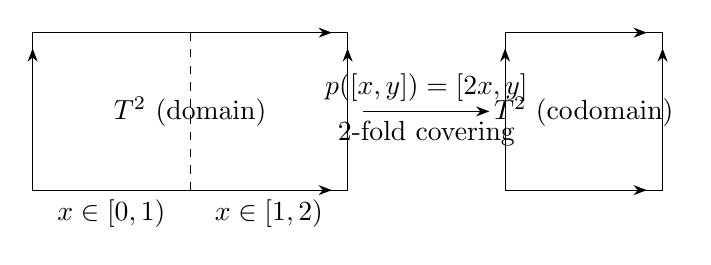
\begin{tikzpicture}[scale=2,>=Stealth]
		
		% Domain: 2x1 rectangle (torus via identifications)
		\begin{scope}
			\draw (0,0) rectangle (2,1);
			\node at (1,0.5) {$T^{2}$ (domain)};
			
			% Horizontal identifications (left-right)
			\draw[->] (0,0.1) -- (0,0.9);
			\draw[->] (2,0.1) -- (2,0.9);
			
			% Vertical identifications (top-bottom, both to the right)
			\draw[->] (0.1,0) -- (1.9,0);
			\draw[->] (0.1,1) -- (1.9,1);
			
			% Mark two fundamental sub-squares
			\draw[dashed] (1,0) -- (1,1);
			\node[below] at (0.5,0) {$x\in[0,1)$};
			\node[below] at (1.5,0) {$x\in[1,2)$};
		\end{scope}
		
		% Codomain: 1x1 square to the right
		\begin{scope}[xshift=3cm]
			\draw (0,0) rectangle (1,1);
			\node at (0.5,0.5) {$T^{2}$ (codomain)};
			
			% Identifications
			\draw[->] (0,0.1) -- (0,0.9);
			\draw[->] (1,0.1) -- (1,0.9);
			\draw[->] (0.1,0) -- (0.9,0);
			\draw[->] (0.1,1) -- (0.9,1);
		\end{scope}
		
		% Arrow indicating 2-fold covering
		\draw[->] (2.1,0.5) -- (2.9,0.5)
		node[midway,above] {$p([x,y]) = [2x,y]$}
		node[midway,below] {$2$-fold covering};
		
	\end{tikzpicture}
	\caption{The covering $p:T^{2}\to T^{2}$ obtained by doubling the first coordinate.}
	\label{fig:T2-to-T2-cover}
\end{figure}

\begin{figure}[h]
	\centering
	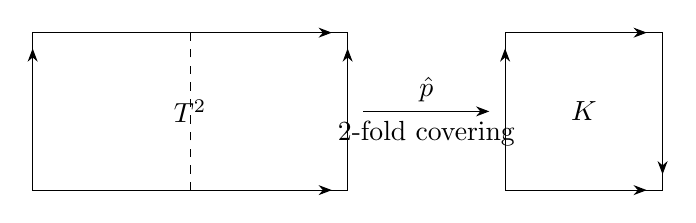
\begin{tikzpicture}[scale=2,>=Stealth]
		
		% Domain: 2x1 rectangle = torus (all sides parallel)
		\begin{scope}
			\draw (0,0) rectangle (2,1);
			\node at (1,0.5) {$T^{2}$};
			
			% Bottom/top arrows
			\draw[->] (0.1,0) -- (1.9,0);
			\draw[->] (0.1,1) -- (1.9,1);
			
			% Left/right arrows
			\draw[->] (0,0.1) -- (0,0.9);
			\draw[->] (2,0.1) -- (2,0.9);
			
			% dashed line splitting into two fundamental domains
			\draw[dashed] (1,0) -- (1,1);
		\end{scope}
		
		% Codomain: Klein bottle square
		\begin{scope}[xshift=3cm]
			\draw (0,0) rectangle (1,1);
			\node at (0.5,0.5) {$K$};
			
			% Bottom/top arrows (same)
			\draw[->] (0.1,0) -- (0.9,0);
			\draw[->] (0.1,1) -- (0.9,1);
			
			% Left/right arrows (opposite)
			\draw[->] (0,0.1) -- (0,0.9);
			\draw[<-] (1,0.1) -- (1,0.9);
		\end{scope}
		
		% Covering arrow
		\draw[->] (2.1,0.5) -- (2.9,0.5)
		node[midway,above] {$\hat p$}
		node[midway,below] {$2$-fold covering};
		
	\end{tikzpicture}
	\caption{The double covering $\hat p:T^{2}\to K$ from the torus to the Klein bottle.}
	\label{fig:T2-to-K-cover}
\end{figure}

\begin{figure}[h]
	\centering
	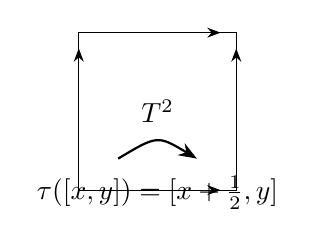
\begin{tikzpicture}[scale=2,>=Stealth]
		
		% Torus square
		\draw (0,0) rectangle (1,1);
		\node at (0.5,0.5) {$T^{2}$};
		
		% Identifications (torus)
		\draw[->] (0.1,0) -- (0.9,0);
		\draw[->] (0.1,1) -- (0.9,1);
		\draw[->] (0,0.1) -- (0,0.9);
		\draw[->] (1,0.1) -- (1,0.9);
		
		% Arrow showing translation x -> x+1/2 (horizontal picture)
		\draw[->,thick] (0.25,0.2) .. controls (0.5,0.35) .. (0.75,0.2);
		\node[below] at (0.5,0.15) {$\tau([x,y])=[x+\tfrac12,y]$};
		
	\end{tikzpicture}
	\caption{The involution $\tau$ on $T^{2}$ given by translation by $(\tfrac12,0)$.
		It has no fixed points.}
	\label{fig:tau-involution}
\end{figure}

\begin{figure}[h]
	\centering
	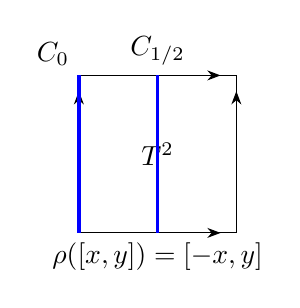
\begin{tikzpicture}[scale=2,>=Stealth]
		
		\draw (0,0) rectangle (1,1);
		\node at (0.5,0.5) {$T^{2}$};
		
		% Identifications
		\draw[->] (0.1,0) -- (0.9,0);
		\draw[->] (0.1,1) -- (0.9,1);
		\draw[->] (0,0.1) -- (0,0.9);
		\draw[->] (1,0.1) -- (1,0.9);
		
		% Fixed circles: x=0 and x=1/2
		\draw[very thick,blue] (0,0) -- (0,1);
		\draw[very thick,blue] (0.5,0) -- (0.5,1);
		
		\node[above left] at (0,1) {$C_{0}$};
		\node[above] at (0.5,1) {$C_{1/2}$};
		
		\node[below] at (0.5,0) {$\rho([x,y])=[-x,y]$};
		
	\end{tikzpicture}
	\caption{The involution $\rho([x,y])=[-x,y]$ with fixed circles $C_{0}$ and $C_{1/2}$.}
	\label{fig:rho-involution}
\end{figure}

\begin{figure}[h]
	\centering
	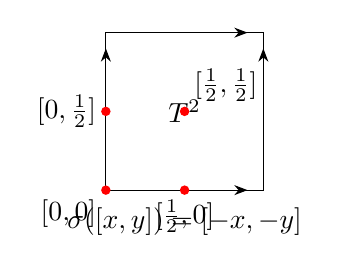
\begin{tikzpicture}[scale=2,>=Stealth]
		
		\draw (0,0) rectangle (1,1);
		\node at (0.5,0.5) {$T^{2}$};
		
		% Identifications
		\draw[->] (0.1,0) -- (0.9,0);
		\draw[->] (0.1,1) -- (0.9,1);
		\draw[->] (0,0.1) -- (0,0.9);
		\draw[->] (1,0.1) -- (1,0.9);
		
		% Four fixed points (0,0), (1/2,0), (0,1/2), (1/2,1/2)
		\foreach \x/\y in {0/0, 0.5/0, 0/0.5, 0.5/0.5} {
			\fill[red] (\x,\y) circle (0.03);
		}
		
		\node[below left]  at (0,0) {$[0,0]$};
		\node[below]       at (0.5,0) {$[\tfrac12,0]$};
		\node[left]        at (0,0.5) {$[0,\tfrac12]$};
		\node[above right] at (0.5,0.5) {$[\tfrac12,\tfrac12]$};
		
		\node[below] at (0.5,-0.05) {$\sigma([x,y])=[-x,-y]$};
		
	\end{tikzpicture}
	\caption{The involution $\sigma([x,y])=[-x,-y]$ with four isolated fixed points.}
	\label{fig:sigma-involution}
\end{figure}


\clearpage

\subsection*{Involutions of the Torus \(T^{2}\)}

We use the standard model
\[
T^{2} = \mathbb{R}^{2}/\mathbb{Z}^{2},
\]
where a point of \(T^{2}\) is denoted by \([x,y]\) with 
\((x,y)\sim(x+m,y+n)\) for integers \(m,n\).

An \emph{involution} is a homeomorphism \(f:T^{2}\to T^{2}\) satisfying 
\(f^{2}=\mathrm{id}\).  
Each involution generates a subgroup 
\(\langle f\rangle\cong\mathbb{Z}/2\subset\mathrm{Homeo}(T^{2})\).

We now describe three involutions with geometrically distinct fixed-point
sets, and therefore defining three pairwise non-conjugate subgroups of 
\(\mathrm{Homeo}(T^{2})\).

\subsubsection*{1. A free translation involution}

\begin{definition}[Translation involution]
	Define
	\[
	\tau([x,y]) = [x+\tfrac12,\,y].
	\]
\end{definition}

\paragraph{Properties.}
Since translation by \((1/2,0)\) followed by itself gives translation 
by \((1,0)\in\mathbb{Z}^{2}\), we have
\[
\tau^{2}([x,y]) = [x+1,y] = [x,y].
\]
Hence \(\tau\) is an involution.

\paragraph{Fixed-point set.}
If \(\tau([x,y])=[x,y]\), then
\[
(x+\tfrac12,y)-(x,y) = (\tfrac12,0)\in\mathbb{Z}^{2},
\]
which is impossible.  
Thus
\[
\mathrm{Fix}(\tau)=\varnothing.
\]
Therefore \(\tau\) acts freely on \(T^{2}\).

\subsubsection*{2. A reflection with two fixed circles}

\begin{definition}[Reflection involution]
	Define
	\[
	\rho([x,y]) = [-x,\,y].
	\]
\end{definition}

\paragraph{Properties.}
Clearly \(\rho^{2}=\mathrm{id}\), so \(\rho\) is an involution.  
This is the reflection across the vertical circles of the torus.

\paragraph{Fixed-point set.}
The condition \(\rho([x,y])=[x,y]\) is equivalent to
\[
(x,y) - (-x,y) = (2x,0)\in\mathbb{Z}^{2}.
\]
Thus \(2x\in\mathbb{Z}\), so \(x\equiv 0\) or \(x\equiv \tfrac12 \pmod{1}\).
Hence
\[
\mathrm{Fix}(\rho)
= \{[0,y] : y\in\mathbb{R}\}
\;\cup\;
\{[\tfrac12,y] : y\in\mathbb{R}\},
\]
a disjoint union of two embedded circles.

\subsubsection*{3. A half-turn rotation with four fixed points}

\begin{definition}[Half-turn involution]
	Define
	\[
	\sigma([x,y]) = [-x,\,-y].
	\]
\end{definition}

\paragraph{Properties.}
Since negating twice gives the identity, we have \(\sigma^{2}=\mathrm{id}\).  
This is a rotation by \(180^\circ\) around the points where both 
coordinates are \(0\) or \(1/2\).

\paragraph{Fixed-point set.}
The condition \(\sigma([x,y])=[x,y]\) becomes
\[
(x,y) - (-x,-y) = (2x,2y)\in\mathbb{Z}^{2}.
\]
Thus \(2x,2y\in\mathbb{Z}\), and
\[
x,y \in \{0,\tfrac12\} \pmod{1}.
\]
Hence the fixed set consists of exactly four points:
\[
\mathrm{Fix}(\sigma)
= \{[0,0], [\tfrac12,0], [0,\tfrac12], [\tfrac12,\tfrac12]\}.
\]

\subsubsection*{Non-conjugacy of the three involutions}

If two involutions \(f,g\in\mathrm{Homeo}(T^{2})\) are conjugate, i.e.
\(
g = h f h^{-1}
\)
for some homeomorphism \(h\), then their fixed-point sets must be
homeomorphic:
\[
\mathrm{Fix}(g) = h(\mathrm{Fix}(f)).
\]

However:
\[
\mathrm{Fix}(\tau)=\varnothing,
\qquad
\mathrm{Fix}(\rho)=\text{two circles},
\qquad
\mathrm{Fix}(\sigma)=\text{four isolated points}.
\]
These three topological types (empty, 1-dimensional, and finite discrete)
are pairwise non-homeomorphic.  
Therefore no homeomorphism of \(T^{2}\) can conjugate one involution into
another, and the three subgroups
\[
\langle\tau\rangle,\qquad 
\langle\rho\rangle,\qquad 
\langle\sigma\rangle 
\;\le\; \mathrm{Homeo}(T^{2})
\]
are pairwise non-conjugate.

\subsection*{Subgroups \(\mathbb{Z}/2 \le \mathrm{Homeo}(T^{2})\) Generated by Involutions}

Throughout we use the model
\[
T^{2} = \mathbb{R}^{2}/\mathbb{Z}^{2}, \qquad [x,y] := (x,y) \bmod \mathbb{Z}^{2}.
\]
An involution is a homeomorphism \(f:T^{2}\to T^{2}\) satisfying \(f^{2}=\mathrm{id}\);
it generates a subgroup \(\langle f\rangle\cong\mathbb{Z}/2\subset\mathrm{Homeo}(T^{2})\).
We describe three such subgroups, each with distinct geometric behaviour.

%-------------------------------------------------------------------
\subsubsection*{1. The translation involution \(\tau\) (free action)}

\begin{definition}[Translation involution]
	Define
	\[
	\tau([x,y]) = [x+\tfrac12,\,y].
	\]
\end{definition}

\paragraph{The subgroup.}
\[
\langle \tau \rangle = \{\mathrm{id},\tau\} \cong \mathbb{Z}/2,
\]
since \(\tau^{2}([x,y]) = [x+1,y]=[x,y]\).


\paragraph{Diagram.}
\begin{figure}[h!]
	\centering
	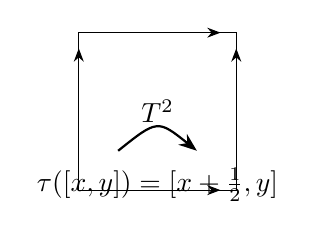
\begin{tikzpicture}[scale=2,>=Stealth]
		% Torus square
		\draw (0,0) rectangle (1,1);
		\node at (0.5,0.5) {$T^{2}$};
		
		% Identifications
		\draw[->] (0.1,0) -- (0.9,0);
		\draw[->] (0.1,1) -- (0.9,1);
		\draw[->] (0,0.1) -- (0,0.9);
		\draw[->] (1,0.1) -- (1,0.9);
		
		% Translation arrow
		\draw[->,thick] (0.25,0.25) .. controls (0.5,0.45) .. (0.75,0.25);
		\node[below] at (0.5,0.2) {$\tau([x,y])=[x+\tfrac12,y]$};
	\end{tikzpicture}
	\caption{The involution \(\tau\). The action is free (no fixed points).}
\end{figure}

\paragraph{Fixed-point set.}
If \(\tau([x,y])=[x,y]\), then \((x+\tfrac12,y)-(x,y)=(\tfrac12,0)\in\mathbb{Z}^{2}\),
a contradiction.  
Hence
\[
\mathrm{Fix}(\tau)=\varnothing,
\]
and \(\tau\) acts freely on \(T^{2}\).

\paragraph{Orbit structure.}
Each orbit consists of two points:
\[
[x,y] \sim [x+\tfrac12,y].
\]

\paragraph{Quotient space.}
Since the action is free and properly discontinuous,
the quotient
\[
T^{2}/\langle\tau\rangle
\]
is again a torus.  
The natural projection \(T^{2}\to T^{2}/\langle\tau\rangle\) is a regular
\(2\)-fold covering map.

%-------------------------------------------------------------------
\subsubsection*{2. The reflection involution \(\rho\) (two fixed circles)}

\begin{definition}[Reflection involution]
	Define
	\[
	\rho([x,y]) = [-x,\,y].
	\]
\end{definition}

\paragraph{The subgroup.}
\[
\langle \rho \rangle = \{\mathrm{id},\rho\} \cong \mathbb{Z}/2,
\]
since \(\rho^{2}=\mathrm{id}\).


\paragraph{Diagram.}
\begin{figure}[h!]
	\centering
	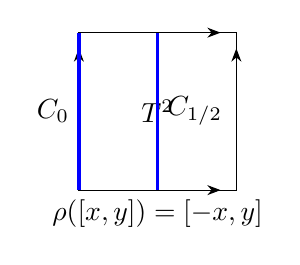
\begin{tikzpicture}[scale=2,>=Stealth]
		
		% Torus square
		\draw (0,0) rectangle (1,1);
		\node at (0.5,0.5) {$T^{2}$};
		
		% Identifications
		\draw[->] (0.1,0) -- (0.9,0);
		\draw[->] (0.1,1) -- (0.9,1);
		\draw[->] (0,0.1) -- (0,0.9);
		\draw[->] (1,0.1) -- (1,0.9);
		
		% Fixed circles
		\draw[very thick,blue] (0,0) -- (0,1);
		\draw[very thick,blue] (0.5,0) -- (0.5,1);
		
		\node[left] at (0,0.5) {$C_0$};
		\node[right] at (0.5,0.5) {$C_{1/2}$};
		
		\node[below] at (0.5,0) {$\rho([x,y])=[-x,y]$};
		
	\end{tikzpicture}
	\caption{The involution \(\rho\). Fixed set consists of two circles.}
\end{figure}

\paragraph{Fixed-point set.}
Solving \([x,y]=[-x,y]\) gives
\[
(x,y)-(-x,y)=(2x,0)\in\mathbb{Z}^{2}
\quad\Longrightarrow\quad
2x\in\mathbb{Z}.
\]
Hence \(x\equiv 0\) or \(x\equiv \tfrac12\pmod{1}\).  
Thus
\[
\mathrm{Fix}(\rho)
= \{[0,y]:y\in\mathbb{R}\}
\;\cup\;
\{[\tfrac12,y]:y\in\mathbb{R}\},
\]
a disjoint union of two embedded circles.

\paragraph{Orbit structure.}
For \(x\not\equiv 0,\tfrac12\), the orbit has two points:
\[
[x,y] \sim [-x,y].
\]
On the two fixed circles each orbit consists of a single point.

\paragraph{Quotient space.}
Geometrically, the action folds the torus along the reflection plane.
The quotient
\[
T^{2}/\langle\rho\rangle
\]
is a cylinder (annulus).  
The projection is \(2\)-to-\(1\) except along the two fixed circles,
where it is \(1\)-to-\(1\).

%-------------------------------------------------------------------
\subsubsection*{3. The half-turn involution \(\sigma\) (four fixed points)}

\begin{definition}[Half-turn involution]
	Define
	\[
	\sigma([x,y]) = [-x,\,-y].
	\]
\end{definition}

\paragraph{The subgroup.}
\[
\langle \sigma \rangle = \{\mathrm{id},\sigma\} \cong \mathbb{Z}/2,
\]
since negating twice gives the identity.


\paragraph{Diagram.}
\begin{figure}[h!]
	\centering
	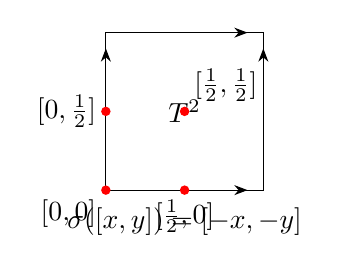
\begin{tikzpicture}[scale=2,>=Stealth]
		
		% Torus square
		\draw (0,0) rectangle (1,1);
		\node at (0.5,0.5) {$T^{2}$};
		
		% Identifications
		\draw[->] (0.1,0) -- (0.9,0);
		\draw[->] (0.1,1) -- (0.9,1);
		\draw[->] (0,0.1) -- (0,0.9);
		\draw[->] (1,0.1) -- (1,0.9);
		
		% Fixed points
		\foreach \x/\y in {0/0,0.5/0,0/0.5,0.5/0.5}
		\fill[red] (\x,\y) circle (0.03);
		
		\node[below left] at (0,0) {$[0,0]$};
		\node[below] at (0.5,0) {$[\tfrac12,0]$};
		\node[left] at (0,0.5) {$[0,\tfrac12]$};
		\node[above right] at (0.5,0.5) {$[\tfrac12,\tfrac12]$};
		
		\node[below] at (0.5,-0.05) {$\sigma([x,y])=[-x,-y]$};
		
	\end{tikzpicture}
	\caption{The involution \(\sigma\). Fixed set consists of four isolated points.}
\end{figure}

\paragraph{Fixed-point set.}
Solving \([x,y]=[-x,-y]\) gives
\[
(x,y)-(-x,-y) = (2x,2y)\in\mathbb{Z}^{2}
\quad\Longrightarrow\quad
x,y\in\{0,\tfrac12\}.
\]
Thus
\[
\mathrm{Fix}(\sigma)
= 
\{[0,0],\,[\tfrac12,0],\,[0,\tfrac12],\,[\tfrac12,\tfrac12]\},
\]
four isolated points.

\paragraph{Orbit structure.}
Away from the four fixed points, each orbit has two elements:
\[
[x,y] \sim [-x,-y].
\]

\paragraph{Quotient space.}
The quotient
\[
T^{2}/\langle\sigma\rangle
\]
is a \(2\)-to-\(1\) map except at the four fixed points,
which become branch (cone) points of order \(2\).
Topologically, the quotient is a surface with four orbifold singularities
coming from the fixed points.

%-------------------------------------------------------------------
\subsubsection*{Non-conjugacy of the three subgroups}

If \(h\in\mathrm{Homeo}(T^{2})\) conjugates one involution to another,
i.e.\ \(hfh^{-1}=g\), then \(h\) maps \(\mathrm{Fix}(f)\) homeomorphically
onto \(\mathrm{Fix}(g)\).

However,
\[
\mathrm{Fix}(\tau)=\varnothing,\qquad
\mathrm{Fix}(\rho)=\text{two circles},\qquad
\mathrm{Fix}(\sigma)=\{4\text{ isolated points}\},
\]
which are pairwise non-homeomorphic sets.  
Thus none of the three subgroups
\[
\langle\tau\rangle,\ \langle\rho\rangle,\ \langle\sigma\rangle
\]
can be conjugate in \(\mathrm{Homeo}(T^{2})\).

\section*{Problem 3}

Draw inside the identification square for the Klein bottle $K$ the set of points
at which the ‘usual’ map \( f : K \to \mathbb{R}^{3} \)
(as drawn on the right above) fails to be injective.
By considering a map
\[
h = (f,\eta) : K \longrightarrow \mathbb{R}^{3} \times \mathbb{R},
\]
where \(\eta\) is a function of the width co-ordinate of the square,
explain why \(K\) can be continuously embedded in \(\mathbb{R}^{4}\),
i.e.\ there is a continuous map \(K \to \mathbb{R}^{4}\) which is a homeomorphism
onto its image.
\emph{[You do not need an explicit formula for \(f\). Many helpful pictures
	can be found at \texttt{https://en.wikipedia.org/wiki/Klein\_bottle}.]}


\section*{Problem 3}

Draw inside the identification square for the Klein bottle $K$ the set of points
at which the ‘usual’ map $f : K \to \mathbb{R}^{3}$
(as drawn on the right above) fails to be injective.
By considering a map
\[
h = (f,\eta) : K \longrightarrow \mathbb{R}^{3} \times \mathbb{R},
\]
where $\eta$ is a function of the width co-ordinate of the square,
explain why $K$ can be continuously embedded in $\mathbb{R}^{4}$,
i.e.\ there is a continuous map $K \to \mathbb{R}^{4}$ which is a homeomorphism
onto its image.
\emph{[You do not need an explicit formula for $f$. Many helpful pictures
	can be found at \texttt{https://en.wikipedia.org/wiki/Klein\_bottle}.]}

\subsection*{Relevant theory: the Klein bottle}

\begin{definition}[Klein bottle]
	The \emph{Klein bottle} $K$ is the quotient of the unit square
	$[0,1]\times[0,1]$ by the identifications
	\[
	(0,y) \sim (1,y) \quad \text{for all } y\in[0,1],
	\]
	and
	\[
	(x,0) \sim (1-x,1) \quad \text{for all } x\in[0,1].
	\]
	The first identification glues the left and right edges of the square with
	the same orientation, and the second glues the bottom and top edges with a
	reversal of orientation.
\end{definition}

\begin{figure}[h]
	\centering
	
\includegraphics[width=\textwidth]{klein_construction_steps.png}
	\caption{Step–by–step construction of the usual immersed Klein bottle:
		from the identification square, through the cylinder, to the self-intersecting
		tube picture in $\mathbb{R}^3$.}
	\label{fig:klein-construction-steps}
\end{figure}


The resulting space $K$ is a closed, non-orientable surface with Euler
characteristic $\chi(K)=0$.  It is a classical fact that $K$ cannot be embedded
in $\mathbb{R}^3$ without self-intersections, but it admits an \emph{immersion}
$f : K \to \mathbb{R}^3$ whose image is the familiar “picture” of the Klein
bottle, where a tube passes through another part of the surface.

In this usual picture, there is a 1-dimensional subset (a closed curve) along
which the surface intersects itself.  Equivalently, there is a curve
$D \subset K$ such that $f$ is injective away from $D$, and for each
$p \in D$ the fibre $f^{-1}(f(p))$ consists of exactly two distinct points.

In terms of the square model $[0,1]\times[0,1]$, with co-ordinates $(x,y)$,
one can describe $K$ as the quotient of this square, and view the immersion
$f$ as a map which (up to the identifications) is injective except along two
distinct curves in the square that are mapped to the same curve in
$\mathbb{R}^3$.  These two curves correspond to two disjoint loops in $K$ that
meet only in their image under $f$.

\subsection*{Solution}

\paragraph{Where $f$ fails to be injective.}
By construction of the usual immersion $f : K \to \mathbb{R}^3$, there is a
closed curve in the image where the surface passes through itself.  For each
point on this self-intersection curve in $\mathbb{R}^3$, there are exactly two
distinct preimages in $K$.  Thus the set
\[
D := \{ p \in K : \# f^{-1}(f(p)) = 2 \}
\]
is a 1-dimensional subset of $K$ (topologically a circle), and $f$ is injective
on $K \setminus D$.

In the identification square $[0,1]\times[0,1]$, with co-ordinates $(x,y)$,
the set $D$ can be represented by two disjoint curves
$C_1, C_2 \subset [0,1]\times[0,1]$ which project to $D$ under the quotient
map.  Each point of $C_1$ and the corresponding point of $C_2$ (with the same
image under the quotient) is mapped by $f$ to the same point of the
self-intersection curve in $\mathbb{R}^3$.  Thus, in the quotient $K$, every
point of $D$ has exactly two preimages for $f$.

Moreover, these two preimages can be chosen to have distinct width co-ordinates:
if we write points in the square as $(x,y)$, then along the two curves
$C_1$ and $C_2$ we have
\[
(x_1(y),y) \in C_1, \qquad (x_2(y),y) \in C_2, \qquad x_1(y) \neq x_2(y),
\]
and these pairs of points project to the double points of $f$ in $K$.

\paragraph{Construction of an embedding in $\mathbb{R}^{4}$}

Let $x : K \to [0,1]/\!\sim$ denote the width co-ordinate induced from the square
model.  Choose a continuous function
\[
\eta : [0,1] \longrightarrow \mathbb{R}
\]
which is strictly monotone (for instance $\eta(t) = t$).  We can regard
$\eta$ as a continuous function on $K$ via the width co-ordinate $x$.

Define
\[
h : K \longrightarrow \mathbb{R}^3 \times \mathbb{R} \cong \mathbb{R}^4,
\qquad
h(p) := \bigl(f(p), \eta(x(p))\bigr).
\]


\begin{itemize}
	\item \emph{Continuity.}
	The map $f$ is continuous, and $\eta \circ x$ is a continuous function
	on $K$, hence $h$ is continuous.
	
	\item \emph{Injectivity.}
	Suppose $h(p_1) = h(p_2)$ for some $p_1,p_2\in K$.  Then
	\[
	f(p_1) = f(p_2)
	\quad\text{and}\quad
	\eta(x(p_1)) = \eta(x(p_2)).
	\]
	If $f(p_1) \neq f(p_2)$, we immediately have a contradiction, so assume
	$f(p_1) = f(p_2)$.  Then $p_1$ and $p_2$ must lie in the double-point set
	$D$, so they belong to the two different sheets of the self-intersection.
	In particular, they have distinct width co-ordinates:
	\[
	x(p_1) \neq x(p_2).
	\]
	Since $\eta$ is strictly monotone, it follows that
	$\eta(x(p_1)) \neq \eta(x(p_2))$, contradicting
	$\eta(x(p_1)) = \eta(x(p_2))$.  Hence such distinct $p_1,p_2$ cannot
	exist, and $h$ is injective.
	
	\item \emph{$h$ is an embedding.}
	The Klein bottle $K$ is compact, and $\mathbb{R}^4$ is Hausdorff.
	A continuous injective map from a compact space to a Hausdorff space
	is a homeomorphism onto its image.  Therefore $h$ is a topological
	embedding of $K$ into $\mathbb{R}^4$.
\end{itemize}

Thus the map $h = (f,\eta) : K \to \mathbb{R}^4$ gives a continuous embedding
of the Klein bottle into $\mathbb{R}^4$, as required.

% In the preamble:
% \usepackage{tikz}
% \usetikzlibrary{arrows.meta}

\begin{figure}[h]
	\centering
	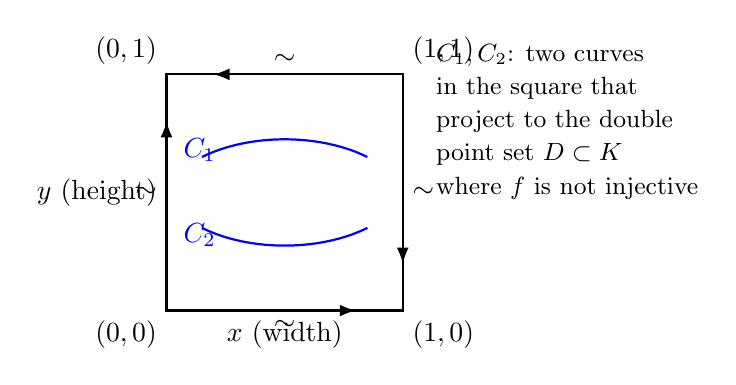
\begin{tikzpicture}[scale=3]
		
		% The square
		\draw[thick] (0,0) rectangle (1,1);
		
		% Coordinates labels
		\node[below left] at (0,0) {$(0,0)$};
		\node[below right] at (1,0) {$(1,0)$};
		\node[above left] at (0,1) {$(0,1)$};
		\node[above right] at (1,1) {$(1,1)$};
		
		% Axes labels (width x, height y)
		\node[below] at (0.5,0) {$x$ (width)};
		\node[left] at (0,0.5) {$y$ (height)};
		
		% Horizontal edge identifications: (0,y) ~ (1,y)
		\draw[-{Latex[length=2mm]}] (0,0.2) -- (0.0,0.8);
		\draw[-{Latex[length=2mm]}] (1,0.8) -- (1.0,0.2);
		\node[left] at (0,0.5) {$\sim$};
		\node[right] at (1,0.5) {$\sim$};
		
		% Vertical edge identifications with flip: (x,0) ~ (1-x,1)
		% arrows showing opposite orientation
		\draw[-{Latex[length=2mm]}] (0.2,0) -- (0.8,0);
		\draw[-{Latex[length=2mm]}] (0.8,1.0) -- (0.2,1.0);
		\node[below] at (0.5,0) {$\sim$};
		\node[above] at (0.5,1) {$\sim$};
		
		% Two curves C1 and C2 where f is non-injective
		% (purely schematic)
		\draw[thick,blue,rounded corners=1pt]
		(0.15,0.65) .. controls (0.35,0.75) and (0.65,0.75) .. (0.85,0.65);
		
		\draw[thick,blue,rounded corners=1pt]
		(0.15,0.35) .. controls (0.35,0.25) and (0.65,0.25) .. (0.85,0.35);
		
		\node[blue] at (0.14,0.68) {$C_1$};
		\node[blue] at (0.14,0.32) {$C_2$};
		
		% Legend / explanation
		\node[align=left,anchor=west] at (1.1,0.8) {%
			\small $C_1, C_2$: two curves\\
			\small in the square that\\
			\small project to the double\\
			\small point set $D \subset K$\\
			\small where $f$ is not injective
		};
		
	\end{tikzpicture}
	\caption{Identification square for the Klein bottle and the preimage
		of the self-intersection of the usual immersion $f:K\to\mathbb{R}^3$.}
	\label{fig:klein-square-double-points}
\end{figure}

\subsection*{1. Intuition: what you actually draw in the square}

We do not need the exact formula for $f$, but conceptually:

\begin{itemize}
	\item In the usual picture in $\mathbb{R}^3$, the Klein bottle has \emph{one self-intersection circle} where a tube passes through itself.
	\item That circle comes from two \emph{distinct simple closed curves} on the surface $K$: think of them as two “loops” that cross in $3$--space but are disjoint on the abstract surface.
\end{itemize}

In the \emph{identification square}:

\begin{itemize}
	\item Take the square with coordinates $(x,y)\in[0,1]\times[0,1]$.
	\item Horizontal identification: $(0,y)\sim(1,y)$.
	\item Vertical identification with flip: $(x,0)\sim(1-x,1)$.
\end{itemize}

Inside this square, choose two simple curves, say

\[
C_1:\ \text{a wiggly curve roughly in the upper part}, \qquad
C_2:\ \text{a wiggly curve roughly in the lower part},
\]

such that:

\begin{itemize}
	\item They are \emph{disjoint} in the square.
	\item After applying the identifications, they become two \emph{disjoint loops in $K$}.
	\item Under the usual immersion $f$, these loops map to the \emph{same circle} in $\mathbb{R}^3$.
\end{itemize}

Therefore, the set where $f$ is not injective is:

\begin{itemize}
	\item In the \textbf{square}: the union $C_1\cup C_2$,
	\item In the \textbf{surface $K$}: the corresponding loop $D\subset K$ (a single circle, since $C_1$ and $C_2$ glue to one loop),
	\item In \textbf{$\mathbb{R}^3$}: the self-intersection circle.
\end{itemize}

Thus, when asked to “draw inside the identification square the set of points where $f$ fails to be injective”, one literally draws the two curves $C_1$ and $C_2$ inside the square, together with the arrows showing the edge identifications.

\bigskip

\subsection*{2. A small useful theory block: immersion vs embedding}

\begin{definition}[Immersion]
	A smooth map $f : M \to \mathbb{R}^n$ from a surface $M$ is an \emph{immersion}
	if its differential has full rank at every point.  
	An immersion may have self-intersections globally.
\end{definition}

\begin{definition}[Embedding]
	A continuous map $F : M \to \mathbb{R}^n$ is a \emph{topological embedding}
	if it is continuous, injective, and a homeomorphism onto its image.
\end{definition}

For the Klein bottle:

\begin{itemize}
	\item The standard figure in $\mathbb{R}^3$ is an \emph{immersion} 
	$f : K \to \mathbb{R}^3$ with a self-intersection circle, so not an embedding.
	\item The trick with 
	\[
	h = (f,\eta) : K \to \mathbb{R}^3\times\mathbb{R}\cong\mathbb{R}^4
	\]
	is that adding the function $\eta$ (depending on the width coordinate) 
	\emph{separates the two sheets} at each double point of $f$.
\end{itemize}

Thus $h$ becomes injective, and since $K$ is compact and $\mathbb{R}^4$ is Hausdorff,
$h$ is automatically a homeomorphism onto its image—hence an \emph{embedding}.


\subsection*{Immersions and embeddings}

\begin{definition}[Immersion]
	Let $M$ be a smooth surface and $f : M \to \mathbb{R}^n$ a smooth map.
	We say that $f$ is an \emph{immersion} if its differential
	$\mathrm{d}f_p : T_pM \to T_{f(p)}\mathbb{R}^n$ has full rank
	(i.e.\ rank $2$) at every point $p\in M$.  An immersion is locally
	an embedding but it may have self-intersections globally.
\end{definition}

\begin{definition}[Embedding]
	A continuous map $F : M \to \mathbb{R}^n$ is a \emph{topological embedding}
	if it is injective and a homeomorphism onto its image $F(M)$ (with the
	subspace topology).  If $M$ is a smooth manifold and $F$ is also a smooth
	immersion, one often speaks of a \emph{smooth embedding}.
\end{definition}

For the Klein bottle $K$, the usual picture in $\mathbb{R}^3$ is given by an
immersion $f : K \to \mathbb{R}^3$ with a self-intersection curve.  The map
\[
h = (f,\eta) : K \longrightarrow \mathbb{R}^3 \times \mathbb{R}
\cong \mathbb{R}^4,
\]
with $\eta$ depending on the width co-ordinate and chosen so that distinct
points in the double point set of $f$ have distinct $\eta$-values, is a
continuous injective map.  Since $K$ is compact and $\mathbb{R}^4$ is
Hausdorff, $h$ is a homeomorphism of $K$ onto its image and thus an embedding
of $K$ into $\mathbb{R}^4$.

\begin{definition}[Topological embedding]
	A continuous map $F : M \to \mathbb{R}^n$ is a \emph{topological embedding}
	if it is injective and a homeomorphism onto its image $F(M)$
	(with the subspace topology).
	If $F$ is also a smooth immersion, one often calls it a \emph{smooth embedding}.
\end{definition}

\paragraph{Immersion of the Klein bottle in $\mathbb{R}^3$.}
The familiar picture of the Klein bottle in $\mathbb{R}^3$ is obtained from a
smooth map
\[
f : K \longrightarrow \mathbb{R}^3,
\]
constructed by gluing a cylinder with a twist. 
This map is a smooth immersion: near every point of $K$, the surface looks
locally like an embedded surface in $\mathbb{R}^3$.  
However, globally $f(K)$ contains a self-intersection curve where one tube
passes through another.  
Hence $f$ is \emph{not} an embedding, because
\[
\# f^{-1}(q) = 2 \quad \text{for all } q \text{ on the self-intersection circle}.
\]

\paragraph{Separating the double points in higher dimension.}
The obstruction to embedding $K$ into $\mathbb{R}^3$ lies entirely in these
double points.  
If we could assign an additional coordinate that takes \emph{different values}
on the two preimages of every self-intersection point, then the map would
become injective.

This is accomplished by introducing a fourth coordinate that depends only on
the width co-ordinate of the square model of $K$.  
This leads to a map
\[
h = (f,\eta) : K \longrightarrow \mathbb{R}^3 \times \mathbb{R}
\cong \mathbb{R}^4,
\]
which is injective and hence (by compactness of $K$ and Hausdorffness of
$\mathbb{R}^4$) a topological embedding.

Thus the Klein bottle, although not embeddable in $\mathbb{R}^3$, embeds
smoothly and naturally in $\mathbb{R}^4$.

\section*{Problem 4}

\begin{enumerate}[label=\textnormal{(\alph*)}]
	
	\item 
	Consider a decomposition of a topological surface into polygons
	(with \(V\) vertices, \(E\) edges and \(F\) faces), where all vertices
	have valence \(\ge 3\) and every face contains \(\ge 3\) vertices.
	Let \(F_{n}\) denote the number of faces bounded by precisely \(n\) edges,
	and \(V_{m}\) the number of vertices where precisely \(m\) edges meet.
	Show that
	\[
	\sum_{n} n F_{n} = 2E = \sum_{m} m V_{m}.
	\]
	If \(V_{3} = 0\), deduce \(E \ge 2V\).
	If \(F_{3} = 0\), deduce \(E \ge 2F\).
	If the surface is a sphere, deduce that \(V_{3} + F_{3} > 0\).
	
	\item 
	For a polygonal decomposition of a sphere, further show that
	\[
	\sum_{n} (6-n) F_{n}
	= 12 + 2 \sum_{m} (m-3) V_{m}.
	\]
	If each face has at least \(3\) edges and at least \(3\) edges meet
	at each vertex, deduce that
	\[
	3F_{3} + 2F_{4} + F_{5} \ge 12.
	\]
	
	\item
	The surface of a football is decomposed into hexagons and pentagons,
	with precisely \(3\) faces meeting at each vertex.
	How many pentagons are there?
	
\end{enumerate}
\section*{Problem 4}

\begin{enumerate}[label=\textnormal{(\alph*)}]
	
	% ------------------------------------------------------------
	% (a)
	% ------------------------------------------------------------
	\item 
	Consider a decomposition of a topological surface into polygons
	(with $V$ vertices, $E$ edges and $F$ faces), where all vertices
	have valence $\ge 3$ and every face contains $\ge 3$ vertices.
	Let $F_{n}$ denote the number of faces bounded by precisely $n$ edges,
	and $V_{m}$ the number of vertices where precisely $m$ edges meet.
	Show that
	\[
	\sum_{n} n F_{n} = 2E = \sum_{m} m V_{m}.
	\]
	If $V_{3} = 0$, deduce $E \ge 2V$.
	If $F_{3} = 0$, deduce $E \ge 2F$.
	If the surface is a sphere, deduce that $V_{3} + F_{3} > 0$.
	
	\medskip
	\textbf{Solution.}
	Each edge is contained in exactly two faces.  
	Counting incidences (face, edge on that face) in two ways yields
	\[
	\sum_n nF_n = 2E.
	\]
	Similarly, each edge has two endpoints.  Counting incidences
	(vertex, edge incident at that vertex) gives
	\[
	\sum_m mV_m = 2E.
	\]
	Hence
	\[
	\sum_n nF_n = 2E = \sum_m mV_m.
	\]
	
	If $V_3 = 0$ and each vertex has valence at least $3$, then every vertex
	has valence at least $4$, so
	\[
	2E = \sum_m mV_m \ge 4V,
	\]
	and therefore $E \ge 2V$.
	
	If $F_3 = 0$ and each face has at least $3$ edges, then each face has at least
	$4$ edges, so
	\[
	2E = \sum_n nF_n \ge 4F,
	\]
	hence $E \ge 2F$.
	
	If the surface is the sphere, Euler’s formula
	\[
	V - E + F = 2
	\]
	holds. If $V_3 = F_3 = 0$, then $E \ge 2V$ and $E \ge 2F$, so
	$V \le E/2$ and $F \le E/2$. Thus
	\[
	V - E + F \le \frac{E}{2} - E + \frac{E}{2} = 0,
	\]
	contradicting $V - E + F = 2$.  
	Hence $V_3 + F_3 > 0$.
	
	% ------------------------------------------------------------
	% (b)
	% ------------------------------------------------------------
	\item
	For a polygonal decomposition of a sphere, show that
	\[
	\sum_{n} (6-n) F_{n}
	= 12 + 2 \sum_{m} (m-3) V_{m}.
	\]
	If each face has at least $3$ edges and at least $3$ edges meet
	at each vertex, deduce that
	\[
	3F_{3} + 2F_{4} + F_{5} \ge 12.
	\]
	
	\medskip
	\textbf{Solution.}
	We compute
	\[
	\sum_n (6-n)F_n
	= 6\sum_n F_n - \sum_n nF_n
	= 6F - 2E,
	\]
	since $\sum_n F_n = F$ and $\sum_n nF_n = 2E$.
	
	Similarly,
	\[
	\sum_m (m-3)V_m
	= \sum_m mV_m - 3\sum_m V_m
	= 2E - 3V,
	\]
	because $\sum_m mV_m = 2E$ and $\sum_m V_m = V$.
	
	Hence
	\[
	12 + 2\sum_m (m-3)V_m
	= 12 + 2(2E - 3V)
	= 12 + 4E - 6V.
	\]
	
	Using Euler’s formula $V - E + F = 2$ on the sphere, we have
	$F = 2 - V + E$. Thus
	\[
	6F - 2E
	= 6(2 - V + E) - 2E
	= 12 - 6V + 4E.
	\]
	Thus
	\[
	\sum_n (6-n)F_n = 12 + 2\sum_m (m-3)V_m.
	\]
	
	If each face has at least 3 edges and each vertex has valence at least 3,
	then $(m-3)V_m \ge 0$ for all $m$, so
	\[
	\sum_n (6-n)F_n \ge 12.
	\]
	Now
	\[
	\sum_n (6-n)F_n
	= 3F_3 + 2F_4 + F_5 + 0\cdot F_6 
	+ \sum_{n\ge 7} (6-n)F_n.
	\]
	For $n \ge 6$, the terms $(6-n)$ are nonpositive, so
	\[
	3F_3 + 2F_4 + F_5 \ge 12.
	\]
	
	% ------------------------------------------------------------
	% (c)
	% ------------------------------------------------------------
	\item
	The surface of a football is decomposed into hexagons and pentagons,
	with precisely $3$ faces meeting at each vertex.
	How many pentagons are there?
	
	\medskip
	\textbf{Solution.}
	Faces are only pentagons and hexagons, so $F_n=0$ unless $n=5,6$.
	Each vertex has valence $3$, so $V_3 = V$ and $V_m = 0$ for $m \ne 3$.
	
	Using the identity proved in (b),
	\[
	\sum_n (6-n)F_n = 12 + 2\sum_m (m-3)V_m.
	\]
	Since $m-3=0$ for $m=3$, the right-hand side is simply $12$.
	
	The left-hand side is
	\[
	(6-5)F_5 + (6-6)F_6 = F_5.
	\]
	Hence $F_5 = 12$.
\end{enumerate}

	\section*{Problem 5}
	
	\begin{enumerate}[label=\textnormal{(\alph*)}]
		
		\item
		Let $S^2 \subset \mathbb{R}^3$ be the unit sphere.
		Let $\pi_{\pm} : S^2 \setminus \{(0,0,\pm 1)\} \to \mathbb{R}^2 = \{z=0\}$
		denote stereographic projection from the north / south poles $(0,0,\pm1)\in S^2$.
		Show that the transition function between these two charts is given by
		\[
		(u,v) \longmapsto \left( \frac{u}{u^{2}+v^{2}}, \frac{v}{u^{2}+v^{2}} \right).
		\]
		Deduce that this atlas gives $S^2$ the structure of an abstract smooth surface.
		
		\item
		Now consider the chart on $S^2$ given by $(U,\phi)$ where
		$U = \{ y < 0 \}$ and $\phi : U \to \mathbb{R}^2$ maps
		$(x,y,z) \mapsto (x,z)$.
		What is the image of $\phi$?
		Check explicitly that this chart is compatible with the smooth atlas defined
		by $\pi_{\pm}$, i.e.\ the transition functions for the atlas with charts
		$\{\pi_{+},\pi_{-},\phi\}$ are all smooth.
		
		\item
		Let $a : S^2 \to S^2$ denote the antipodal map, $x \mapsto -x$.
		Show that $a$ is a diffeomorphism of the abstract smooth surface $S^2$, and
		deduce that the real projective plane $\mathbb{R}P^{2}$ also admits the
		structure of an abstract smooth surface.
		
	\end{enumerate}
	
	

	\begin{enumerate}[label=\textnormal{(\alph*)}]
		
		\item
		Let $S^2 \subset \mathbb{R}^3$ be the unit sphere.
		Let $\pi_{\pm} : S^2 \setminus \{(0,0,\pm 1)\} \to \mathbb{R}^2 = \{z=0\}$
		denote stereographic projection from the north / south poles $(0,0,\pm1)\in S^2$.
		Show that the transition function between these two charts is given by
		\[
		(u,v) \longmapsto \left( \frac{u}{u^{2}+v^{2}}, \frac{v}{u^{2}+v^{2}} \right).
		\]
		Deduce that this atlas gives $S^2$ the structure of an abstract smooth surface.
		
		\medskip
		\textbf{Solution.}
		For $(x,y,z)\in S^2$ with $z\neq 1$ the stereographic projection from the north
		pole is
		\[
		\pi_+(x,y,z) = \left(\frac{x}{1-z}, \frac{y}{1-z}\right),
		\]
		and from the south pole
		\[
		\pi_-(x,y,z) = \left(\frac{x}{1+z}, \frac{y}{1+z}\right),
		\]
		both with inverses defined on $\mathbb{R}^2$.
		For $(u,v)\in\mathbb{R}^2$ write $r^2 = u^2+v^2$.  Then
		\[
		\pi_+^{-1}(u,v)
		= \left(
		\frac{2u}{1+r^2},
		\frac{2v}{1+r^2},
		\frac{r^2-1}{1+r^2}
		\right).
		\]
		Hence
		\[
		\pi_- \circ \pi_+^{-1}(u,v)
		= \left(
		\frac{\frac{2u}{1+r^2}}{1+\frac{r^2-1}{1+r^2}},
		\frac{\frac{2v}{1+r^2}}{1+\frac{r^2-1}{1+r^2}}
		\right)
		= \left(
		\frac{u}{r^2},
		\frac{v}{r^2}
		\right)
		= \left(
		\frac{u}{u^{2}+v^{2}},
		\frac{v}{u^{2}+v^{2}}
		\right)
		\]
		on $\mathbb{R}^2 \setminus \{0\}$.  This map and its inverse are smooth,
		so the two charts $\pi_+$ and $\pi_-$ are smoothly compatible, and they define
		an atlas giving $S^2$ the structure of an abstract smooth surface.
		
		\medskip
		
		\item
		Now consider the chart on $S^2$ given by $(U,\phi)$ where
		$U = \{ y < 0 \}$ and $\phi : U \to \mathbb{R}^2$ maps $(x,y,z) \mapsto (x,z)$.
		What is the image of $\phi$?
		Check explicitly that this chart is compatible with the smooth atlas defined
		by $\pi_{\pm}$, i.e.\ the transition functions for the atlas with charts
		$\{\pi_{+},\pi_{-},\phi\}$ are all smooth.
		
		\medskip
		\textbf{Solution.}
		If $(x,y,z)\in S^2$, then $x^2+y^2+z^2=1$.  On $U$ we have $y<0$, hence
		\[
		y = -\sqrt{1-x^2-z^2}
		\]
		and necessarily $x^2+z^2 < 1$.
		Conversely, for any $(u,v)\in\mathbb{R}^2$ with $u^2+v^2<1$ we can define
		\[
		\phi^{-1}(u,v) = \bigl(u,\,-\sqrt{1-u^2-v^2},\,v\bigr) \in U \subset S^2.
		\]
		Thus
		\[
		\phi(U) = \{(u,v)\in\mathbb{R}^2 : u^2+v^2<1\},
		\]
		the open unit disc.
		
		To check compatibility, consider, for instance,
		$\pi_+ \circ \phi^{-1} : \phi(U) \to \mathbb{R}^2$:
		for $(u,v)$ with $u^2+v^2<1$,
		\[
		\phi^{-1}(u,v) = (u,-\sqrt{1-u^2-v^2},v) = (x,y,z),
		\]
		so
		\[
		\pi_+(x,y,z)
		= \left(\frac{x}{1-z},\frac{y}{1-z}\right)
		= \left(
		\frac{u}{1-v},
		\frac{-\sqrt{1-u^2-v^2}}{1-v}
		\right).
		\]
		Here $1-v>0$ on the unit disc, and the right-hand side is clearly a smooth
		function of $(u,v)$.  Similarly
		\[
		\pi_-(x,y,z)
		= \left(
		\frac{u}{1+v},
		\frac{-\sqrt{1-u^2-v^2}}{1+v}
		\right)
		\]
		is smooth on the disc.  The maps $\phi \circ \pi_\pm^{-1}$ are compositions
		of these with the inverses $\pi_\pm^{-1}$, hence are smooth.
		Thus $\phi$ is smoothly compatible with $\pi_\pm$, and the atlas
		$\{\pi_+,\pi_-,\phi\}$ is a smooth atlas on $S^2$.
		
		\medskip
		
		\item
		Let $a : S^2 \to S^2$ denote the antipodal map, $x \mapsto -x$.
		Show that $a$ is a diffeomorphism of the abstract smooth surface $S^2$, and
		deduce that the real projective plane $\mathbb{R}P^{2}$ also admits the
		structure of an abstract smooth surface.
		
		\medskip
		\textbf{Solution.}
		The map $A:\mathbb{R}^3\to\mathbb{R}^3$, $A(x)=-x$, is linear and hence
		smooth, and it restricts to a map $a=S^2\to S^2$.  To see that $a$ is smooth
		as a map of the abstract smooth surface $S^2$, consider its local expression
		in the stereographic charts:
		\[
		\Phi_+ := \pi_+ \circ a \circ \pi_+^{-1} : \mathbb{R}^2 \to \mathbb{R}^2.
		\]
		Both $\pi_+^{-1}$ and $\pi_+$ are smooth, as is $a$ in $\mathbb{R}^3$, so
		$\Phi_+$ is smooth.  The same argument applies for $\pi_-$.  Since
		$a^{-1}=a$ has the same coordinate expressions, the inverse is also smooth.
		Thus $a$ is a diffeomorphism of $S^2$.
		
		Define an equivalence relation on $S^2$ by $x\sim -x$, and write
		$\mathbb{R}P^2 = S^2/\sim$ for the set of equivalence classes.
		The action of the group $\mathbb{Z}_2 = \{ \mathrm{id}, a\}$ on $S^2$ is
		smooth, free and properly discontinuous.  For any chart $(U,\varphi)$ on
		$S^2$ with $U\cap a(U)=\varnothing$, the projection
		$q:S^2\to\mathbb{R}P^2$ restricts to a homeomorphism of $U$ onto $q(U)$, and
		we can use $\varphi$ as a coordinate map on $q(U)$ via this identification.
		Transition maps between such charts on $\mathbb{R}P^2$ are induced by the
		transition maps on $S^2$, and hence are smooth.
		
		Therefore $\mathbb{R}P^2$ admits an atlas of compatible smooth charts and
		thus carries the structure of an abstract smooth surface.
	\end{enumerate}
	
	
	\begin{figure}[h]
		\centering
		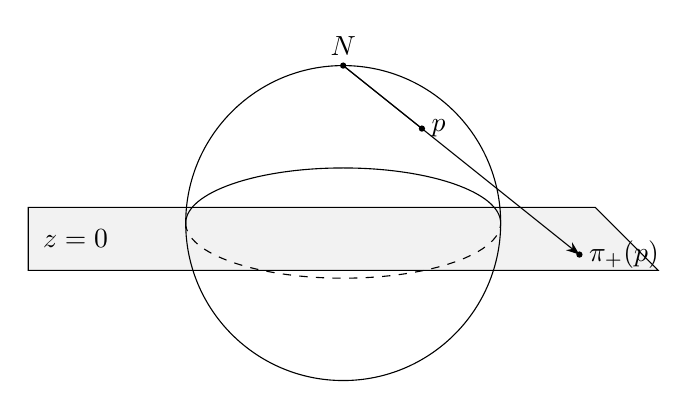
\begin{tikzpicture}[scale=2, >=Stealth]
			
			% Plane z = 0 as a tilted rectangle
			\fill[gray!10]
			(-2,-0.3) -- (2,-0.3) -- (1.6,0.1) -- (-2,0.1) -- cycle;
			\draw
			(-2,-0.3) -- (2,-0.3) -- (1.6,0.1) -- (-2,0.1) -- cycle;
			\node at (-1.7,-0.1) {$z=0$};
			
			% Sphere
			\draw (0,0) circle (1);
			
			% Equator (ellipse: front solid, back dashed)
			\draw (-1,0) arc (180:0:1 and 0.35);           % front
			\draw[dashed] (-1,0) arc (180:360:1 and 0.35); % back
			
			% North pole N
			\coordinate (N) at (0,1);
			\fill (N) circle (0.02);
			\node[above] at (N) {$N$};
			
			% Point p on the upper hemisphere
			\coordinate (P) at (0.5,0.6);
			\fill (P) circle (0.02);
			\node[right] at (P) {$p$};
			
			% Image of p under stereographic projection from N
			% Direction from N to P is (0.5, -0.4); extend until y = -0.2
			% 1 + t*(-0.4) = -0.2  => t = 3, so point is (1.5, -0.2).
			\coordinate (Q) at (1.5,-0.2);
			\fill (Q) circle (0.02);
			\node[right] at (Q) {$\pi_+(p)$};
			
			% Line from N through p to the plane
			\draw (N) -- (P);
			\draw[->] (N) -- (Q);
			
		\end{tikzpicture}
		\caption{Stereographic projection $\pi_+$ from the north pole $N$ onto the plane $z=0$.}
		\label{fig:stereographic-tikz}
	\end{figure}
	
	


	
	\section*{Problem 6 — Intersection of Two Surfaces Gives a Smooth Curve}
	
	A \emph{smooth curve} in $\mathbb{R}^3$ is a subspace which can locally be
	given as the image of a smooth injective map
	\[
	(-1,1) \to \mathbb{R}^3
	\]
	with injective differential.
	
	Let
	\[
	H : \mathbb{R}^3 \to \mathbb{R},
	\qquad
	K : \mathbb{R}^3 \to \mathbb{R}
	\]
	be smooth functions.
	Suppose the level sets
	\[
	H^{-1}(0)
	\qquad\text{and}\qquad
	K^{-1}(0)
	\]
	are smooth surfaces in $\mathbb{R}^3$ which intersect along a smooth curve
	$\gamma$.
	
	Let $p = (x_0,y_0,z_0) \in \gamma$, and assume that at $p$ the expression
	\[
	K_y H_z \;-\; K_z H_y
	\]
	is non-vanishing.
	
	Show that, in some neighbourhood of $p$, the curve $\gamma$ can be parametrized
	by the variable $x$.  If we write
	\[
	\gamma(x) = (x, y(x), z(x)),
	\]
	then prove that
	\[
	y'(x)
	= \frac{K_z H_x - K_x H_z}{K_y H_z - K_z H_y}.
	\]
	
	\bigskip
	
	
	\subsection*{Smooth Curves: Definition and Charts}
	
	A subset $\gamma \subset \mathbb{R}^3$ is called a \emph{smooth curve} if
	every point $p\in\gamma$ has a neighbourhood $U\subset\gamma$ for which there
	exists a smooth injective map
	\[
	\alpha : (-1,1) \longrightarrow \mathbb{R}^3
	\]
	with non-vanishing derivative $\alpha'(t)\neq 0$ such that
	$\alpha((-1,1)) = U$.
	Thus a smooth curve is a $1$--dimensional embedded smooth submanifold of
	$\mathbb{R}^3$.
	
	\subsection*{Regular parametrizations}
	A smooth map $\alpha : I \to \mathbb{R}^3$ is a \emph{regular
		parametrization} if $\alpha'(t)\neq 0$ for all $t\in I$.
	If $\alpha$ is regular, then $\gamma=\alpha(I)$ is a smooth curve, and
	conversely every smooth curve is locally the image of a regular parametrization.
	
	\subsection*{Charts on a smooth curve}
	Let $\gamma$ be a smooth curve and let
	$\alpha : I \to \gamma$ be a regular parametrization.
	Then
	\[
	\varphi = \alpha^{-1} : U=\alpha(I) \to I
	\]
	defines a smooth chart on $U$.
	Transition maps between such charts are smooth because changes of
	parametrization are smooth.
	Hence every smooth curve carries a natural structure of a $1$--dimensional
	smooth manifold.
	
	\subsection*{Geometric sources of smooth curves}
	\begin{itemize}
		\item Intersections of smooth surfaces $H^{-1}(0)\cap K^{-1}(0)$,
		provided the gradients are transverse.
		\item Level sets $f^{-1}(c)$ in $\mathbb{R}^2$ with $\nabla f \neq 0$.
		\item Images of regular embeddings $\alpha : \mathbb{R}\to\mathbb{R}^3$.
	\end{itemize}
	
	 \emph{smooth curve} in $\mathbb{R}^3$ is a subspace which can locally be
	given as the image of a smooth injective map
	\[
	(-1,1) \to \mathbb{R}^3
	\]
	with injective differential.
	
	Let
	\[
	H : \mathbb{R}^3 \to \mathbb{R}, \qquad
	K : \mathbb{R}^3 \to \mathbb{R}
	\]
	be smooth functions.
	Suppose the level sets
	\[
	H^{-1}(0) \quad\text{and}\quad K^{-1}(0)
	\]
	are smooth surfaces in $\mathbb{R}^3$ which intersect along a smooth curve
	$\gamma$.
	Suppose $p = (x_0,y_0,z_0)$ belongs to $\gamma$, and that at $p$ the expression
	$K_y H_z - K_z H_y$ is non-vanishing.
	
	\begin{enumerate}[label=\textnormal{(\alph*)}]
		\item Show that in some neighbourhood of $p$ the curve $\gamma$ can be
		parametrized by the variable $x$, and that if we write
		\[
		\gamma(x) = (x,y(x),z(x)),
		\]
		then
		\[
		y'(x) = \frac{K_z H_x - K_x H_z}{K_y H_z - K_z H_y}.
		\]
	\end{enumerate}
	
	\medskip
	
	\textbf{Solution.}
	Define
	\[
	F : \mathbb{R}^3 \to \mathbb{R}^2, \qquad
	F(x,y,z) = \bigl(H(x,y,z),\,K(x,y,z)\bigr).
	\]
	Then $\gamma$ is exactly the zero set of $F$,
	\[
	\gamma = F^{-1}(0,0),
	\]
	and at the point $p=(x_0,y_0,z_0)$ we have
	\[
	K_y H_z - K_z H_y \neq 0.
	\]
	Consider the Jacobian of $F$ with respect to the variables $(y,z)$:
	\[
	D_{(y,z)}F(x,y,z)
	=
	\begin{pmatrix}
		H_y & H_z \\
		K_y & K_z
	\end{pmatrix}.
	\]
	Its determinant is
	\[
	\det D_{(y,z)}F
	= H_y K_z - H_z K_y
	= -(K_y H_z - K_z H_y),
	\]
	which is non-zero at $p$ by assumption.  Therefore, by the implicit function
	theorem, there exist an open interval $I$ containing $x_0$ and smooth
	functions $y,z : I \to \mathbb{R}$ such that
	\[
	F\bigl(x,y(x),z(x)\bigr) = (0,0)
	\]
	for all $x\in I$.  In particular, near $p$ the intersection curve $\gamma$ is
	parametrized by
	\[
	\gamma(x) = \bigl(x,y(x),z(x)\bigr),
	\]
	so $x$ is a valid parameter.
	
	Since for all $x\in I$ we have
	\[
	H\bigl(x,y(x),z(x)\bigr) = 0,
	\qquad
	K\bigl(x,y(x),z(x)\bigr) = 0,
	\]
	differentiating with respect to $x$ yields
	\begin{align*}
		H_x + H_y\,y'(x) + H_z\,z'(x) &= 0, \\
		K_x + K_y\,y'(x) + K_z\,z'(x) &= 0.
	\end{align*}
	This is a linear system for the unknowns $y'(x)$ and $z'(x)$:
	\[
	\begin{cases}
		H_y\,y' + H_z\,z' = -H_x,\\
		K_y\,y' + K_z\,z' = -K_x.
	\end{cases}
	\]
	Let
	\[
	\Delta = \det
	\begin{pmatrix}
		H_y & H_z \\
		K_y & K_z
	\end{pmatrix}
	= H_y K_z - H_z K_y
	= -(K_y H_z - K_z H_y) \neq 0.
	\]
	By Cramer's rule, the numerator for $y'$ is
	\[
	\det
	\begin{pmatrix}
		-H_x & H_z \\
		-K_x & K_z
	\end{pmatrix}
	= (-H_x)K_z - H_z(-K_x)
	= H_z K_x - H_x K_z.
	\]
	Thus
	\[
	y'
	= \frac{H_z K_x - H_x K_z}{H_y K_z - H_z K_y}
	= \frac{K_z H_x - K_x H_z}{K_y H_z - K_z H_y},
	\]
	where in the last equality we multiply numerator and denominator by $-1$
	and use commutativity of multiplication.
	This proves the claimed formula.
	
	
	\section*{Problem 7 — Level Sets of a Cubic Surface}
	
	Consider the subset
	\[
	\Sigma \subset \mathbb{R}^3
	\qquad\text{defined by}\qquad
	\Sigma = \{(x,y,z) : z = x^3 + y^3 - 3xy\}.
	\]
	
	\begin{enumerate}[label=\textnormal{(\alph*)}]
		
		\item
		Show that $\Sigma$ is a smooth surface in $\mathbb{R}^3$.
		
		\item
		Show that the level set
		\[
		\Sigma \cap \{z=c\}
		\]
		is a (not necessarily connected) smooth curve in the $(x,y)$–plane
		unless
		\[
		c \in \{-1,0\}.
		\]
		
		\item
		Sketch the level sets for the special values $c=-1$ and $c=0$.
		
		(For $c=-1$, you may use the factorization)
		\[
		x^3 + y^3 - 3xy + 1
		= (x+y+1)\bigl(x^2 + y^2 - xy - x - y + 1\bigr).
		\]
		
	\end{enumerate}
	
	
	\textbf{Solution.}
	
	\paragraph{(a) $\Sigma$ is a smooth surface.}
	Define
	\[
	f(x,y) = x^3 + y^3 - 3xy, \qquad
	F(x,y,z) = z - f(x,y).
	\]
	Then
	\[
	\Sigma = F^{-1}(0).
	\]
	We have
	\[
	\frac{\partial F}{\partial z}(x,y,z) = 1 \neq 0
	\]
	for all $(x,y,z)$.
	By the implicit function theorem, the level set $F^{-1}(0)$ is a smooth
	$2$--dimensional submanifold of $\mathbb{R}^3$; in fact it is the graph of the
	smooth function $f$.  Hence $\Sigma$ is a smooth surface.
	
	\paragraph{(b) Level sets are smooth curves for $c\notin\{-1,0\}$.}
	Fix $c\in\mathbb{R}$ and intersect $\Sigma$ with the plane $z=c$.
	On this plane, points have the form $(x,y,c)$ and satisfy
	\[
	c = x^3 + y^3 - 3xy,
	\]
	or equivalently
	\[
	g_c(x,y) := x^3 + y^3 - 3xy - c = 0.
	\]
	Thus
	\[
	\Sigma \cap \{z=c\}
	= \{(x,y,c) : g_c(x,y)=0\}
	\]
	is naturally identified with the level set $g_c^{-1}(0)\subset\mathbb{R}^2$.
	
	We compute
	\[
	\nabla g_c(x,y) = \bigl(3x^2 - 3y,\; 3y^2 - 3x\bigr),
	\]
	which is independent of $c$.
	The gradient vanishes exactly when
	\[
	3x^2 - 3y = 0, \qquad 3y^2 - 3x = 0
	\quad\Longleftrightarrow\quad
	x^2 = y, \quad y^2 = x.
	\]
	Substituting $y=x^2$ into $y^2=x$ gives
	\[
	x^4 = x \quad\Longleftrightarrow\quad x(x^3-1)=0,
	\]
	so $x=0$ or $x=1$.  Thus the only critical points of $g_c$ are
	\[
	(0,0) \quad\text{and}\quad (1,1).
	\]
	
	We now determine for which $c$ these points lie on the level set $g_c^{-1}(0)$:
	
	\begin{itemize}
		\item At $(0,0)$ we have $x^3 + y^3 - 3xy = 0$, so
		\[
		g_c(0,0) = -c,
		\]
		which vanishes iff $c=0$.
		\item At $(1,1)$ we have $1^3+1^3-3\cdot1\cdot1 = -1$, so
		\[
		g_c(1,1) = -1 - c,
		\]
		which vanishes iff $c=-1$.
	\end{itemize}
	
	Hence, if $c\notin\{-1,0\}$, the level set $g_c^{-1}(0)$ contains no critical
	points of $g_c$, so $\nabla g_c\neq 0$ at every point on $g_c^{-1}(0)$.
	By the implicit function theorem in $\mathbb{R}^2$, each such level set is a
	(possibly disconnected) smooth $1$--dimensional submanifold of
	$\mathbb{R}^2$, i.e.\ a smooth plane curve.  Therefore
	$\Sigma\cap\{z=c\}$ is a smooth curve in the plane for all
	$c\notin\{-1,0\}$.
	
	\paragraph{(c) Sketch for $c=-1$ and $c=0$.}
	
	For $c=-1$ the equation becomes
	\[
	x^3 + y^3 - 3xy + 1 = 0.
	\]
	The given factorisation
	\[
	x^3 + y^3 - 3xy + 1
	= (x+y+1)\bigl(x^2 + y^2 - xy - x - y + 1\bigr)
	\]
	shows that the level set is the union of
	\[
	x + y + 1 = 0
	\]
	(a straight line) and
	\[
	x^2 + y^2 - xy - x - y + 1 = 0,
	\]
	which is an ellipse (the associated quadratic form is positive definite).
	Thus the intersection $\Sigma\cap\{z=-1\}$ consists of a line and a smooth
	oval.
	
	For $c=0$ the equation is
	\[
	x^3 + y^3 - 3xy = 0.
	\]
	The origin $(0,0)$ lies on this level set and is a critical point of $g_0$
	since $\nabla g_0(0,0)=(0,0)$.  Thus the level set $g_0^{-1}(0)$ has a
	singularity at the origin, where several branches of the cubic curve meet.
	Away from $(0,0)$, $\nabla g_0\neq 0$, so the curve is smooth at all other
	points.  Hence $\Sigma\cap\{z=0\}$ is a singular cubic curve passing through
	$(0,0)$, smooth everywhere except at the origin.
	
	
	\begin{figure}[h]
		\centering
		\begin{tikzpicture}[scale=2]
			
			% axes
			\draw[->] (-2,0) -- (2,0) node[right] {$x$};
			\draw[->] (0,-2) -- (0,2) node[above] {$y$};
			
			% level set c = -1: line x + y + 1 = 0
			\draw[thick] (-2,1) -- (1,-2);
			\node[above right] at (-1,0) {$x+y+1=0$};
			
			% ellipse (schematic) for x^2 + y^2 - xy - x - y + 1 = 0
			\draw[thick, domain=0:360, smooth, variable=\t]
			plot ({0.4*cos(\t) + 0.1*sin(\t)}, {0.2*sin(\t) - 0.1*cos(\t)});
			\node at (0.8,1.1) {$x^2 + y^2 - xy - x - y + 1 = 0$};
			
			% label
			\node[below right] at (1.1,-1.6) {$c=-1$};
			
		\end{tikzpicture}
		\caption{Qualitative shape of the level set $x^3 + y^3 - 3xy = -1$:
			it is the union of the line $x+y+1=0$ and a smooth closed oval.}
		\label{fig:c-minus-1}
	\end{figure}
	
	\paragraph{Explanation.}
	For $c=-1$ we have
	\[
	x^3 + y^3 - 3xy + 1 = 0,
	\]
	and the given factorisation
	\[
	x^3 + y^3 - 3xy + 1
	= (x+y+1)\bigl(x^2 + y^2 - xy - x - y + 1\bigr)
	\]
	shows that the level set consists of two components:
	the straight line $x+y+1=0$ and the conic
	\[
	x^2 + y^2 - xy - x - y + 1 = 0,
	\]
	which is an ellipse (since the associated quadratic form is positive
	definite).  Thus $\Sigma\cap\{z=-1\}$ is the union of a line and a smooth
	oval lying in the $(x,y)$–plane.
	
	
\begin{figure}[h]
	\centering
	\begin{tikzpicture}[scale=2]
		
		% axes
		\draw[->] (-1.5,0) -- (1.5,0) node[right] {$x$};
		\draw[->] (0,-1.5) -- (0,1.5) node[above] {$y$};
		
		% schematic branches of the cubic x^3 + y^3 - 3xy = 0
		\draw[thick, smooth]
		(-1.2,-0.2) .. controls (-0.6,-0.1) and (-0.3,-0.05) .. (0,0)
		.. controls (0.3,0.05) and (0.6,0.1) .. (1.2,0.2);
		
		\draw[thick, smooth]
		(-0.2,-1.2) .. controls (-0.1,-0.6) and (-0.05,-0.3) .. (0,0)
		.. controls (0.05,0.3) and (0.1,0.6) .. (0.2,1.2);
		
		\draw[thick, smooth]
		(-1.0,1.0) .. controls (-0.5,0.5) and (-0.2,0.2) .. (0,0)
		.. controls (0.2,-0.2) and (0.5,-0.5) .. (1.0,-1.0);
		
		% mark the singular point
		\fill (0,0) circle (0.03);
		\node[below right] at (0,0) {$(0,0)$};
		
		% label
		\node[below right] at (0.8,-1.3) {$x^3 + y^3 - 3xy = 0$};
		\node[below left] at (-1.3,-1.3) {$c=0$};
		
	\end{tikzpicture}
	\caption{Qualitative sketch of the level set $x^3 + y^3 - 3xy = 0$:
		a cubic curve with a singular point at the origin.}
	\label{fig:c-zero}
\end{figure}

\paragraph{Explanation.}
For $c=0$ the level set is given by
\[
x^3 + y^3 - 3xy = 0.
\]
The origin $(0,0)$ lies on this curve and is a critical point, since
\[
\nabla(x^3 + y^3 - 3xy)(0,0) = (0,0).
\]
Thus the origin is a singular point, where several smooth branches of the
cubic meet.  Away from $(0,0)$ the gradient is non-zero, so the curve is a
smooth $1$--dimensional submanifold of the plane except at this single
singular point.

	
	
	
\section*{Problem E1 — Map Colouring on Surfaces}

\begin{enumerate}[label=\textnormal{(\alph*)}]
	
	\item
	View a polygonal decomposition of a topological surface $S$ with all
	vertices of valence $\ge 3$ as a map drawn on $S$.
	The map can be coloured with $N$ colours if we can colour faces so that
	faces which share an edge have different colours (but faces which meet
	only at a vertex may have the same colour).
	
	Suppose that $N \in \mathbb{N}$ is a positive integer such that
	\[
	\frac{2E}{F} < N
	\]
	for every possible decomposition of $S$ (here $E$ is the number of edges
	and $F$ the number of faces).
	Show that every map on $S$ can be coloured with at most $N$ colours.
	\emph{[Hint: Induct on $F$, noting that the result is straightforward if
		$F < N$.]}
	
	\item
	Prove that for any decomposition of $S$ (where all vertices have valence
	at least $3$), we have
	\[
	\frac{2E}{F} \le 6\Bigl(1 - \frac{\chi(S)}{F}\Bigr),
	\]
	where $\chi(S)$ is the Euler characteristic of $S$.
	Deduce that any map on a torus can be coloured with $7$ colours.
	
	The map on the torus depicted below can be coloured with $7$ colours but
	not fewer -- why?
	\emph{[The black dots represent the vertices; note the `corner' of the
		rectangle is not one.]}
	
\end{enumerate}

\begin{figure}[h]
	\centering
	
\includegraphics[width=0.7\textwidth]{e1.png}%
	\caption{A map on the torus used in part (b) of Problem E1.
		The black dots represent the vertices; the corner of the rectangle is
		not a vertex.}
	\label{fig:E1-torus-map}
\end{figure}

\subsection*{Valence (Degree) of a Vertex}

Let $G$ be the graph coming from a polygonal decomposition of a surface $S$,
with vertex set $V$ and edge set $E$.

\begin{definition}
	For a vertex $v \in V$, the \emph{valence} (or \emph{degree}) of $v$,
	denoted $\operatorname{val}(v)$, is the number of edges of $G$ which are
	incident with $v$.
	Equivalently, $\operatorname{val}(v)$ is the number of polygon edges that
	meet at $v$ in the decomposition.
\end{definition}

Thus, if three polygon edges meet at a point $v$, then $\operatorname{val}(v)=3$;
if four edges meet at $v$, then $\operatorname{val}(v)=4$, and so on.
(Loops, i.e.\ edges that begin and end at the same vertex, are counted
twice, but such edges usually do not appear in polygonal decompositions.)

In the context of map colouring problems, one usually assumes that all
vertices have valence at least $3$.  This excludes degenerate configurations
and ensures that each vertex is surrounded by at least three faces, so that
Euler characteristic and counting arguments behave nicely.
	
	
	\begin{figure}[h]
		\centering
		
		%%%%% Vertex of valence 3 %%%%%
		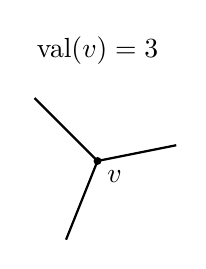
\begin{tikzpicture}[scale=1]
			\node at (0,1.4) {$\operatorname{val}(v)=3$};
			\fill (0,0) circle (0.05) node[below right] {$v$};
			\draw[thick] (0,0) -- (1,0.2);
			\draw[thick] (0,0) -- (-0.8,0.8);
			\draw[thick] (0,0) -- (-0.4,-1.0);
		\end{tikzpicture}
		\hspace{1.5cm}
		%%%%% Vertex of valence 4 %%%%%
		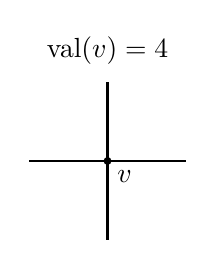
\begin{tikzpicture}[scale=1]
			\node at (0,1.4) {$\operatorname{val}(v)=4$};
			\fill (0,0) circle (0.05) node[below right] {$v$};
			\draw[thick] (0,0) -- (1,0);
			\draw[thick] (0,0) -- (-1,0);
			\draw[thick] (0,0) -- (0,1);
			\draw[thick] (0,0) -- (0,-1);
		\end{tikzpicture}
		\hspace{1.5cm}
		%%%%% Vertex of valence 5 %%%%%
		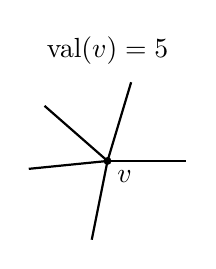
\begin{tikzpicture}[scale=1]
			\node at (0,1.4) {$\operatorname{val}(v)=5$};
			\fill (0,0) circle (0.05) node[below right] {$v$};
			\draw[thick] (0,0) -- (1,0);
			\draw[thick] (0,0) -- (0.3,1.0);
			\draw[thick] (0,0) -- (-0.8,0.7);
			\draw[thick] (0,0) -- (-1.0,-0.1);
			\draw[thick] (0,0) -- (-0.2,-1.0);
		\end{tikzpicture}
		
		\caption{Examples of vertices of valence $3$, $4$, and $5$.
			The valence of a vertex is the number of incident edges.}
		\label{fig:vertex-valences}
	\end{figure}
	
	
\subsection*{Euler Characteristic}

Let $S$ be a surface equipped with a polygonal (or triangulated)
decomposition.
Denote by $V$ the number of vertices, by $E$ the number of edges, and by
$F$ the number of faces (2--cells).

\begin{definition}
	The \emph{Euler characteristic} of $S$ is
	\[
	\chi(S) := V - E + F.
	\]
	A fundamental theorem of topology says that $\chi(S)$ is independent of the
	chosen polygonal decomposition: it is a topological invariant of the
	surface $S$.
\end{definition}

\subsection*{Examples}

\paragraph{Sphere $S^2$.}
Consider a tetrahedron drawn on the sphere.  It has
$V=4$ vertices, $E=6$ edges and $F=4$ triangular faces, so
\[
\chi(S^2) = V - E + F = 4 - 6 + 4 = 2.
\]

\paragraph{Torus $T^2$.}
Represent the torus as a square with opposite sides identified.
Using the standard cell structure, there is
one vertex (all four corners are identified), two edges (one horizontal and
one vertical loop), and one face (the interior of the square).  Hence
\[
\chi(T^2) = 1 - 2 + 1 = 0.
\]

More generally, a closed orientable surface of genus $g$ satisfies
\[
\chi(\Sigma_g) = 2 - 2g.
\]
In particular $S^2$ (genus $0$) has Euler characteristic $2$, the torus
(genus $1$) has Euler characteristic $0$, a double torus (genus $2$) has
Euler characteristic $-2$, and so on.
	
	\begin{figure}[h]
		\centering
		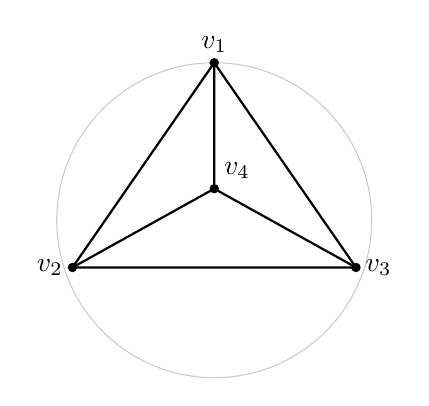
\begin{tikzpicture}[scale=2]
			
			% sphere outline (just for intuition)
			\draw[gray!40] (0,0) circle (1);
			
			% tetrahedron vertices
			\coordinate (A) at (0,1);
			\coordinate (B) at (-0.9,-0.3);
			\coordinate (C) at (0.9,-0.3);
			\coordinate (D) at (0,0.2);
			
			% edges
			\draw[thick] (A)--(B)--(C)--(A);   % outer triangle
			\draw[thick] (A)--(D)--(B);
			\draw[thick] (C)--(D);
			
			% vertices
			\fill (A) circle (0.03) node[above] {$v_1$};
			\fill (B) circle (0.03) node[left] {$v_2$};
			\fill (C) circle (0.03) node[right] {$v_3$};
			\fill (D) circle (0.03) node[above right] {$v_4$};
			
		\end{tikzpicture}
		\caption{A tetrahedron drawn on $S^2$.  Here $V=4$, $E=6$, $F=4$ and
			$\chi(S^2)=4-6+4=2$.}
		\label{fig:euler-sphere}
	\end{figure}
	
	\begin{figure}[h]
		\centering
		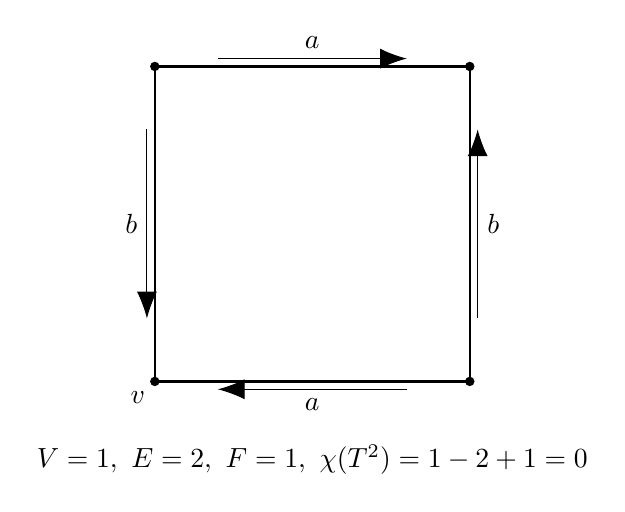
\begin{tikzpicture}[scale=2]
			
			% square
			\draw[thick] (-1,-1) rectangle (1,1);
			
			% arrows indicating identifications
			\draw[->] (-0.6,1.05) -- (0.6,1.05);
			\draw[->] (0.6,-1.05) -- (-0.6,-1.05);
			\node[above] at (0,1.05) {$a$};
			\node[below] at (0,-1.05) {$a$};
			
			\draw[->] (1.05,-0.6) -- (1.05,0.6);
			\draw[->] (-1.05,0.6) -- (-1.05,-0.6);
			\node[right] at (1.05,0) {$b$};
			\node[left]  at (-1.05,0) {$b$};
			
			% single vertex (all corners identified)
			\fill (-1,-1) circle (0.03);
			\fill (1,-1) circle (0.03);
			\fill (1,1) circle (0.03);
			\fill (-1,1) circle (0.03);
			\node[below left] at (-1,-1) {$v$};
			
			% label
			\node at (0,-1.5) {$V=1,\ E=2,\ F=1,\ \chi(T^2)=1-2+1=0$};
			
		\end{tikzpicture}
		\caption{Square with opposite edges identified, giving the torus $T^2$.
			All four corners represent the same vertex $v$, the two independent edge
			loops are labelled $a$ and $b$, and the whole interior is a single face.}
		\label{fig:euler-torus}
	\end{figure}
	
	\begin{figure}[h]
		\centering
		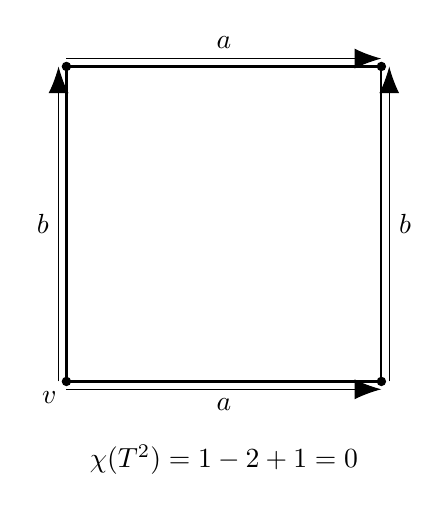
\begin{tikzpicture}[scale=2]
			
			% square
			\draw[thick] (-1,-1) rectangle (1,1);
			
			% horizontal edges (a)
			\draw[->] (-1,1.05) -- (1,1.05);
			\draw[->] (-1,-1.05) -- (1,-1.05);
			\node[above] at (0,1.05) {$a$};
			\node[below] at (0,-1.05) {$a$};
			
			% vertical edges (b)
			\draw[->] (1.05,-1) -- (1.05,1);
			\draw[->] (-1.05,-1) -- (-1.05,1);
			\node[right] at (1.05,0) {$b$};
			\node[left]  at (-1.05,0) {$b$};
			
			% all four corners identified as one vertex
			\fill (-1,-1) circle (0.03);
			\fill (1,-1) circle (0.03);
			\fill (1,1) circle (0.03);
			\fill (-1,1) circle (0.03);
			\node[below left] at (-1,-1) {$v$};
			
			\node at (0,-1.5) {$\chi(T^2) = 1 - 2 + 1 = 0$};
			
		\end{tikzpicture}
		\caption{Square with opposite sides identified to form the torus $T^2$.
			Although opposite edges are drawn with arrows in the same direction, the
			boundary word is $aba^{-1}b^{-1}$ when read anticlockwise.}
		\label{fig:torus-fundamental-square}
	\end{figure}
	
	\begin{figure}[h]
		\centering
		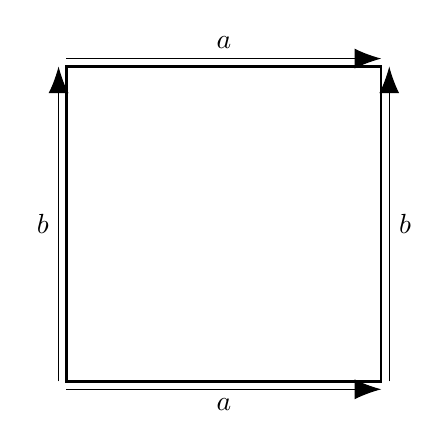
\begin{tikzpicture}[scale=2]
			
			% square
			\draw[thick] (-1,-1) rectangle (1,1);
			
			% horizontal edges labelled a
			\draw[->] (-1,1.05) -- (1,1.05);
			\draw[->] (-1,-1.05) -- (1,-1.05);
			\node[above] at (0,1.05) {$a$};
			\node[below] at (0,-1.05) {$a$};
			
			% vertical edges labelled b
			\draw[->] (1.05,-1) -- (1.05,1);
			\draw[->] (-1.05,-1) -- (-1.05,1);
			\node[right] at (1.05,0) {$b$};
			\node[left]  at (-1.05,0) {$b$};
			
		\end{tikzpicture}
		\caption{Fundamental polygon for the torus. Traversing anticlockwise produces the word $a\,b\,a^{-1}\,b^{-1}$.}
	\end{figure}
	
	
	\begin{figure}[h]
		\centering
		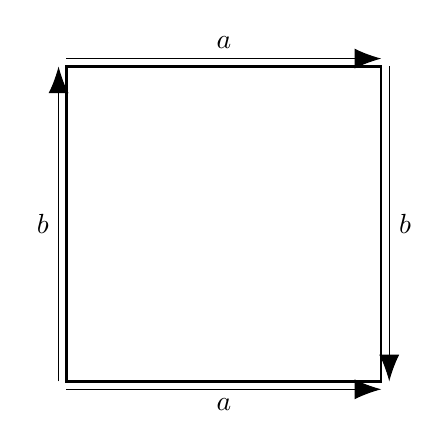
\begin{tikzpicture}[scale=2]
			
			% square
			\draw[thick] (-1,-1) rectangle (1,1);
			
			% horizontal edges labelled a (same orientation)
			\draw[->] (-1,1.05) -- (1,1.05);
			\draw[->] (-1,-1.05) -- (1,-1.05);
			\node[above] at (0,1.05) {$a$};
			\node[below] at (0,-1.05) {$a$};
			
			% vertical edges labelled b, one arrow reversed
			\draw[->] (1.05,1) -- (1.05,-1);      % downward arrow
			\draw[->] (-1.05,-1) -- (-1.05,1);    % upward arrow
			\node[right] at (1.05,0) {$b$};
			\node[left]  at (-1.05,0) {$b$};
			
		\end{tikzpicture}
		\caption{Fundamental polygon for the Klein bottle. Traversal yields $a\,b\,a\,b^{-1}$.}
	\end{figure}
	
	\clearpage
	
	\subsection*{Real projective plane $\mathbb{RP}^2$}
	
	The real projective plane $\mathbb{RP}^2$ can be obtained from a square by
	identifying each pair of opposite edges with reversed orientation.
	A standard cell decomposition has
	\[
	V = 1,\quad E = 1,\quad F = 1,
	\]
	so
	\[
	\chi(\mathbb{RP}^2) = V - E + F = 1 - 1 + 1 = 1.
	\]
	
	\begin{figure}[h]
		\centering
		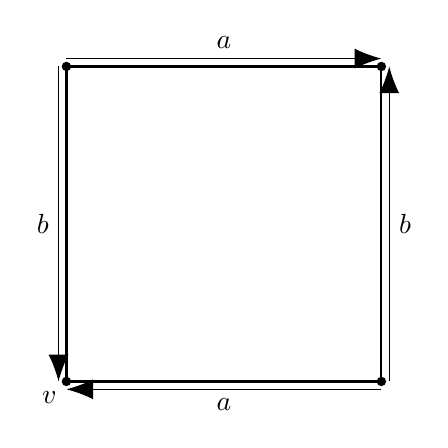
\begin{tikzpicture}[scale=2]
			
			% square
			\draw[thick] (-1,-1) rectangle (1,1);
			
			% horizontal edges (label a, opposite directions)
			\draw[->] (-1,1.05) -- (1,1.05);
			\draw[->] (1,-1.05) -- (-1,-1.05);
			\node[above] at (0,1.05) {$a$};
			\node[below] at (0,-1.05) {$a$};
			
			% vertical edges (label b, opposite directions)
			\draw[->] (1.05,-1) -- (1.05,1);
			\draw[->] (-1.05,1) -- (-1.05,-1);
			\node[right] at (1.05,0) {$b$};
			\node[left]  at (-1.05,0) {$b$};
			
			% corners all identified as one vertex
			\fill (-1,-1) circle (0.03);
			\fill (1,-1) circle (0.03);
			\fill (1,1) circle (0.03);
			\fill (-1,1) circle (0.03);
			\node[below left] at (-1,-1) {$v$};
			
		\end{tikzpicture}
		\caption{Fundamental polygon for $\mathbb{RP}^2$: opposite edges are identified
			with reversed orientation. In a suitable cell decomposition one obtains
			$V=1$, $E=1$, $F=1$ and hence $\chi(\mathbb{RP}^2)=1$.}
		\label{fig:rp2-fundamental}
	\end{figure}
	
	\subsection*{Klein bottle $K$}
	
	The Klein bottle can be represented by a square whose horizontal edges are
	identified with the same orientation and whose vertical edges are
	identified with opposite orientation.  A convenient cell decomposition has
	\[
	V = 1,\quad E = 2,\quad F = 1,
	\]
	so
	\[
	\chi(K) = 1 - 2 + 1 = 0.
	\]
	Although the Euler characteristic agrees with that of the torus, the Klein
	bottle is non-orientable and thus not homeomorphic to $T^2$.
	
	\begin{figure}[h]
		\centering
		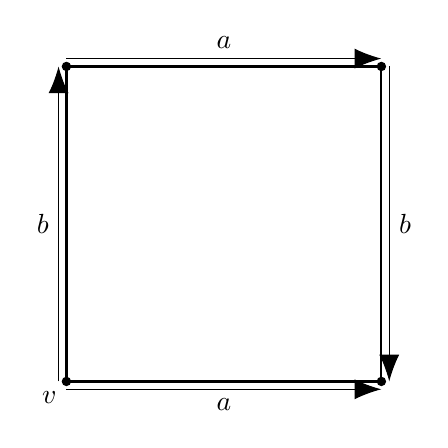
\begin{tikzpicture}[scale=2]
			
			% square
			\draw[thick] (-1,-1) rectangle (1,1);
			
			% horizontal edges (a, same direction)
			\draw[->] (-1,1.05) -- (1,1.05);
			\draw[->] (-1,-1.05) -- (1,-1.05);
			\node[above] at (0,1.05) {$a$};
			\node[below] at (0,-1.05) {$a$};
			
			% vertical edges (b, opposite directions)
			\draw[->] (1.05,1) -- (1.05,-1);
			\draw[->] (-1.05,-1) -- (-1.05,1);
			\node[right] at (1.05,0) {$b$};
			\node[left]  at (-1.05,0) {$b$};
			
			% corners identified
			\fill (-1,-1) circle (0.03);
			\fill (1,-1) circle (0.03);
			\fill (1,1) circle (0.03);
			\fill (-1,1) circle (0.03);
			\node[below left] at (-1,-1) {$v$};
			
		\end{tikzpicture}
		\caption{Fundamental polygon for the Klein bottle $K$: one pair of edges
			is identified with the same orientation, the other pair with reversed
			orientation. A suitable cell structure yields $V=1$, $E=2$, $F=1$ and
			$\chi(K)=0$.}
		\label{fig:klein-fundamental}
	\end{figure}
	
	\subsection*{Double torus $\Sigma_2$}
	
	A closed orientable surface of genus $2$ (a ``double torus'') can be
	represented by an octagon whose edges are labelled
	\[
	a, b, a^{-1}, b^{-1}, c, d, c^{-1}, d^{-1}
	\]
	in order around the boundary.
	All $8$ vertices are identified to a single vertex, and the $8$ edges form
	$4$ pairs corresponding to the loops $a,b,c,d$.  There is a single face
	(the interior of the octagon).  Thus
	\[
	V = 1,\quad E = 4,\quad F = 1,
	\]
	and
	\[
	\chi(\Sigma_2) = 1 - 4 + 1 = -2.
	\]
	This agrees with the general formula for closed orientable surfaces of
	genus $g$:
	\[
	\chi(\Sigma_g) = 2 - 2g.
	\]
	
	\begin{figure}[h]
		\centering
		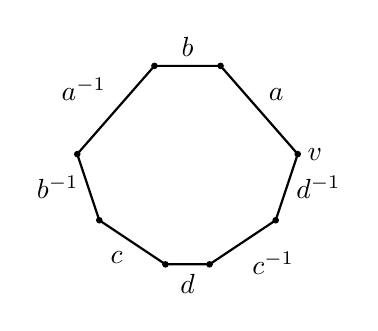
\begin{tikzpicture}[scale=1.4]
			
			% vertices of an octagon
			\coordinate (P1) at (1,0);
			\coordinate (P2) at (0.3,0.8);
			\coordinate (P3) at (-0.3,0.8);
			\coordinate (P4) at (-1,0);
			\coordinate (P5) at (-0.8,-0.6);
			\coordinate (P6) at (-0.2,-1);
			\coordinate (P7) at (0.2,-1);
			\coordinate (P8) at (0.8,-0.6);
			
			% draw octagon
			\draw[thick] (P1)--(P2)--(P3)--(P4)--(P5)--(P6)--(P7)--(P8)--cycle;
			
			% edge labels (schematic)
			\node[above right] at ($(P1)!0.5!(P2)$) {$a$};
			\node[above]       at ($(P2)!0.5!(P3)$) {$b$};
			\node[above left]  at ($(P3)!0.5!(P4)$) {$a^{-1}$};
			\node[left]        at ($(P4)!0.5!(P5)$) {$b^{-1}$};
			\node[below left]  at ($(P5)!0.5!(P6)$) {$c$};
			\node[below]       at ($(P6)!0.5!(P7)$) {$d$};
			\node[below right] at ($(P7)!0.5!(P8)$) {$c^{-1}$};
			\node[right]       at ($(P8)!0.5!(P1)$) {$d^{-1}$};
			
			% all vertices identified: indicate single vertex
			\fill (P1) circle (0.03);
			\fill (P2) circle (0.03);
			\fill (P3) circle (0.03);
			\fill (P4) circle (0.03);
			\fill (P5) circle (0.03);
			\fill (P6) circle (0.03);
			\fill (P7) circle (0.03);
			\fill (P8) circle (0.03);
			\node[right] at (P1) {$v$};
			
		\end{tikzpicture}
		\caption{Fundamental polygon for the genus $2$ surface $\Sigma_2$.
			All $8$ vertices are identified to a single vertex $v$, the $8$ edges form
			$4$ pairs, and the interior is one face, giving $V=1$, $E=4$, $F=1$ and
			$\chi(\Sigma_2) = -2$.}
		\label{fig:double-torus-fundamental}
	\end{figure}
	
	\subsection*{Euler characteristic and the inequality in E1(b)}
	
	Let $S$ be a surface with a polygonal decomposition in which every vertex
	has valence at least $3$.  Denote by $V,E,F$ the numbers of vertices,
	edges and faces respectively, and let $\chi(S) = V - E + F$ be the Euler
	characteristic of $S$.
	
	Write $V_m$ for the number of vertices of valence $m$.  Then
	\[
	\sum_m V_m = V,
	\qquad
	\sum_m mV_m = 2E,
	\]
	and the assumption on valences implies $V_m=0$ for $m<3$.  Hence
	\[
	2E = \sum_m mV_m \;\ge\; \sum_m 3V_m = 3V,
	\]
	so that
	\[
	V \le \frac{2E}{3}.
	\]
	
	On the other hand, the Euler characteristic may be written as
	\[
	\chi(S) = V - E + F
	\quad\Longrightarrow\quad
	F - \chi(S) = E - V.
	\]
	Multiplying by $2$ gives
	\[
	2(F - \chi(S)) = 2E - 2V.
	\]
	Using the bound $V \le 2E/3$ we obtain
	\[
	2E - 2V \;\ge\; 2E - 2\cdot\frac{2E}{3}
	= \frac{2E}{3},
	\]
	and hence
	\[
	2(F - \chi(S)) \;\ge\; \frac{2E}{3}
	\quad\Longrightarrow\quad
	F - \chi(S) \;\ge\; \frac{E}{3}.
	\]
	Equivalently,
	\[
	E \le 3\bigl(F - \chi(S)\bigr).
	\]
	Multiplying both sides by $2/F$ yields
	\[
	\frac{2E}{F} \;\le\;
	\frac{6(F - \chi(S))}{F}
	= 6\Bigl(1 - \frac{\chi(S)}{F}\Bigr),
	\]
	which is precisely the inequality stated in part~(b) of Problem~E1.
	
	\subsection*{Colouring bounds for the sphere and the torus}
	
	Part~(a) of Problem~E1 shows that if there exists an integer $N$ such that
	\[
	\frac{2E}{F} < N
	\]
	for every polygonal decomposition of $S$ (with all vertices of valence
	$\ge 3$), then every map on $S$ can be coloured with at most $N$ colours.
	
	For the sphere $S^2$ we have $\chi(S^2)=2$, and the inequality above
	gives
	\[
	\frac{2E}{F} \le 6\Bigl(1 - \frac{2}{F}\Bigr) < 6
	\]
	for every decomposition.  Thus we may take $N=6$, and every map on $S^2$
	is $6$--colourable (this is the classical six-colour theorem).
	
	For the torus $T^2$ we have $\chi(T^2)=0$, so the inequality reduces to
	\[
	\frac{2E}{F} \le 6.
	\]
	Hence any $N>6$ satisfies $\frac{2E}{F} < N$ for all decompositions; in
	particular we may choose $N=7$ and conclude that every map on the torus is
	$7$--colourable.  The specific example drawn in Problem~E1 shows a map on
	the torus which cannot be coloured with fewer than $7$ colours, so this
	bound is sharp.
	
	\clearpage
	
	\subsection*{Examples of Euler characteristics}
	
	For reference, the Euler characteristics of some standard closed surfaces
	are collected in Table~\ref{tab:euler-surfaces}.
	
	\begin{table}[h]
		\centering
		\begin{tabular}{lcc}
			\hline
			Surface $S$ & Description & $\chi(S)$ \\
			\hline
			$S^2$ & sphere (genus $0$)          & $2$ \\
			$T^2$ & torus (genus $1$)           & $0$ \\
			$\Sigma_2$ & double torus (genus $2$) & $-2$ \\
			$\mathbb{RP}^2$ & real projective plane & $1$ \\
			$K$ & Klein bottle                  & $0$ \\
			\hline
		\end{tabular}
		\caption{Euler characteristics of some standard closed surfaces.}
		\label{tab:euler-surfaces}
	\end{table}
	
	
	\subsubsection*{Solution to E1(a)}
	
	We prove the statement by induction on the number of faces $F$ in the map.
	
	Recall that a map on $S$ is given by a polygonal decomposition with $V$
	vertices, $E$ edges and $F$ faces, and that by assumption there exists a
	fixed integer $N \in \mathbb{N}$ such that
	\[
	\frac{2E}{F} < N
	\]
	for every such decomposition of $S$.
	
	\paragraph{Base case: $F < N$.}
	Suppose first that $F < N$.
	The adjacency graph of faces has at most $F$ vertices, and each face has
	at most $F-1$ neighbours (it cannot share an edge with itself).
	We can therefore colour the faces greedily with $N$ colours as follows:
	list the faces as $F_1,\dots,F_F$, and colour them one by one.
	When we come to colour $F_k$, at most $k-1 \le F-1 < N$ neighbours have
	already been assigned colours, so at most $N-1$ colours are forbidden.
	Since there are $N$ colours available, at least one colour remains,
	and we may assign it to $F_k$.
	Thus any map with $F < N$ is $N$--colourable.
	
	\paragraph{Inductive step.}
	Assume now that every map on $S$ with fewer than $F$ faces is
	$N$--colourable, and let $M$ be a map on $S$ with $F$ faces, $E$ edges,
	and satisfying
	\[
	\frac{2E}{F} < N.
	\]
	We must show that $M$ is $N$--colourable.
	
	Let $F_n$ denote the number of faces of $M$ which are bounded by exactly
	$n$ edges.  Then
	\[
	F = \sum_n F_n,
	\qquad
	\sum_n nF_n = 2E,
	\]
	since each edge is incident with exactly two faces.
	Hence the average number of edges per face is
	\[
	\frac{1}{F}\sum_n nF_n
	= \frac{2E}{F}
	< N.
	\]
	If every face had at least $N$ edges, then the average would be at least
	$N$, which contradicts the inequality above.
	Therefore there exists at least one face $f$ which has at most $N-1$
	edges.
	
	Remove this face $f$ from the map, leaving a new map $M'$ on $S$ with
	\[
	F' = F-1
	\]
	faces.  (Some edges may now bound only one face, but this does not affect
	the argument.)
	By the hypothesis on $N$, the inequality
	\[
	\frac{2E'}{F'} < N
	\]
	holds for \emph{every} decomposition of $S$, and in particular for $M'$.
	Thus, by the inductive hypothesis, $M'$ is $N$--colourable.
	
	Consider the face $f$ which we removed.  It is incident with at most
	$N-1$ distinct neighbouring faces (since it has at most $N-1$ edges), and
	these neighbours are already coloured in $M'$.
	Among the $N$ available colours, at most $N-1$ are used on these
	neighbours, so there is at least one colour which does not appear among
	them.
	Assign such a colour to $f$.
	Then adjacent faces always have distinct colours, and we have obtained an
	$N$--colouring of the original map $M$.
	
	By induction on $F$, every map on $S$ can be coloured with at most $N$
	colours.

	
	\begin{figure}[h]
		\centering
		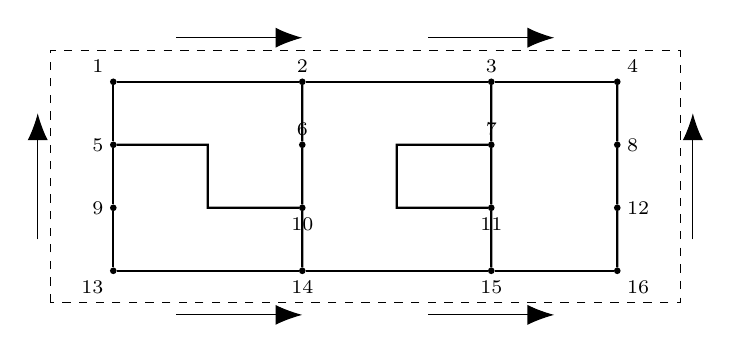
\begin{tikzpicture}[scale=0.8, every node/.style={font=\scriptsize}]
			
			% Fundamental rectangle (torus)
			\draw[dashed] (0,0) rectangle (10,4);
			
			% Identification arrows (left-right)
			\draw[->] (2,4.2) -- (4,4.2);
			\draw[->] (6,4.2) -- (8,4.2);
			\draw[->] (2,-0.2) -- (4,-0.2);
			\draw[->] (6,-0.2) -- (8,-0.2);
			
			% Identification arrows (bottom-top)
			\draw[->] (-0.2,1) -- (-0.2,3);
			\draw[->] (10.2,1) -- (10.2,3);
			
			% --- vertices (roughly matching a 7-hexagon tiling) ---
			
			% top row
			\node[inner sep=1pt] (v1)  at (1,3.5)  {};
			\node[inner sep=1pt] (v2)  at (4,3.5)  {};
			\node[inner sep=1pt] (v3)  at (7,3.5)  {};
			\node[inner sep=1pt] (v4)  at (9,3.5)  {};
			
			% upper middle row
			\node[inner sep=1pt] (v5)  at (1,2.5)  {};
			\node[inner sep=1pt] (v6)  at (4,2.5)  {};
			\node[inner sep=1pt] (v7)  at (7,2.5)  {};
			\node[inner sep=1pt] (v8)  at (9,2.5)  {};
			
			% lower middle row
			\node[inner sep=1pt] (v9)  at (1,1.5)  {};
			\node[inner sep=1pt] (v10) at (4,1.5)  {};
			\node[inner sep=1pt] (v11) at (7,1.5)  {};
			\node[inner sep=1pt] (v12) at (9,1.5)  {};
			
			% bottom row
			\node[inner sep=1pt] (v13) at (1,0.5)  {};
			\node[inner sep=1pt] (v14) at (4,0.5)  {};
			\node[inner sep=1pt] (v15) at (7,0.5)  {};
			\node[inner sep=1pt] (v16) at (9,0.5)  {};
			
			% draw the dots
			\foreach \v in {1,...,16}{
				\fill (v\v) circle (1.5pt);
			}
			
			% labels (you can shift them slightly if needed)
			\node[above left]  at (v1)  {$1$};
			\node[above]       at (v2)  {$2$};
			\node[above]       at (v3)  {$3$};
			\node[above right] at (v4)  {$4$};
			
			\node[left]        at (v5)  {$5$};
			\node[above]       at (v6)  {$6$};
			\node[above]       at (v7)  {$7$};
			\node[right]       at (v8)  {$8$};
			
			\node[left]        at (v9)  {$9$};
			\node[below]       at (v10) {$10$};
			\node[below]       at (v11) {$11$};
			\node[right]       at (v12) {$12$};
			
			\node[below left]  at (v13) {$13$};
			\node[below]       at (v14) {$14$};
			\node[below]       at (v15) {$15$};
			\node[below right] at (v16) {$16$};
			
			% --- edges (just a schematic network) ---
			
			% top zig-zag
			\draw[thick] (v1) -- (v2) -- (v3) -- (v4);
			% left verticals
			\draw[thick] (v1) -- (v5) -- (v9) -- (v13);
			% middle verticals
			\draw[thick] (v2) -- (v6) -- (v10) -- (v14);
			\draw[thick] (v3) -- (v7) -- (v11) -- (v15);
			% right verticals
			\draw[thick] (v4) -- (v8) -- (v12) -- (v16);
			% bottom zig-zag
			\draw[thick] (v13) -- (v14) -- (v15) -- (v16);
			
			% two interior “bends” to suggest the hexagonal regions
			\draw[thick] (v5) -- (2.5,2.5) -- (2.5,1.5) -- (v10);
			\draw[thick] (v7) -- (5.5,2.5) -- (5.5,1.5) -- (v11);
			
		\end{tikzpicture}
		\caption{A schematic torus map with vertices labelled.
			The left/right and top/bottom edges of the rectangle are identified.}
		\label{fig:torus-map-labelled}
	\end{figure}
	
	\clearpage
	
\section{The Real Projective Plane \texorpdfstring{$\mathbb{RP}^2$}{RP2}}

\subsection{Definitions of $\mathbb{RP}^2$}

There are several equivalent ways to define the real projective plane.  
Each illuminates a different geometric property of $\mathbb{RP}^2$.

\begin{definition}[As Lines Through the Origin in $\mathbb{R}^3$]
	The real projective plane is the space of 1-dimensional linear subspaces of
	$\mathbb{R}^3$.  Two nonzero vectors $v,w \in \mathbb{R}^3$ represent the same
	point of $\mathbb{RP}^2$ if $w = \lambda v$ for some nonzero real number
	$\lambda$.  
	
	Every point of $\mathbb{RP}^2$ may be written using homogeneous coordinates:
	\[
	[x:y:z] = [\lambda x : \lambda y : \lambda z], \qquad \lambda \neq 0.
	\]
	
	Thus
	\[
	\mathbb{RP}^2 = (\mathbb{R}^3 \setminus \{0\}) / \!\sim ,
	\qquad v \sim w \Longleftrightarrow w = \lambda v \text{ for some } \lambda \ne 0.
	\]
\end{definition}

\begin{definition}[Affine Plane with Line at Infinity]
	Embed the affine plane $\mathbb{R}^2$ into projective space by
	\[
	(x,y) \longmapsto [x : y : 1].
	\]
	The points with $z=0$ are the \emph{points at infinity}:
	\[
	[x : y : 0] \in \mathbb{RP}^2 \setminus \mathbb{R}^2.
	\]
	They represent directions of parallel lines in the affine plane.
	
	Therefore,
	\[
	\mathbb{RP}^2 = \mathbb{R}^2 \ \cup\  \mathbb{RP}^1,
	\]
	where $\mathbb{RP}^1$ is the \emph{projective line at infinity}.
\end{definition}

\begin{definition}[Sphere Modulo Antipodal Identification]
	Let
	\[
	S^2 = \{ (x,y,z)\in\mathbb{R}^3 : x^2 + y^2 + z^2 = 1 \}.
	\]
	Define an equivalence relation by $(x,y,z) \sim (-x,-y,-z)$.
	Then
	\[
	\mathbb{RP}^2 \cong S^2 / (x \sim -x).
	\]
	
	This model shows immediately that $\mathbb{RP}^2$ is compact, non-orientable,
	and obtained from a sphere by identifying opposite points.
\end{definition}

\subsection{Geometric Interpretation and Examples}

\begin{example}[Finite and Infinite Points]
	A finite affine point $(x,y)\in\mathbb{R}^2$ corresponds to $[x:y:1]$.
	Points of the form $[x:y:0]$ lie on the \emph{line at infinity}, which
	collects all directions of parallel lines.
	
	Thus, projective geometry removes the concept of parallelism:
	any two distinct projective lines meet at a unique point (possibly at infinity).
\end{example}

\begin{example}[Projective Lines]
	A projective line is the set of solutions to a homogeneous linear equation
	\[
	ax + by + cz = 0,
	\quad (a,b,c) \neq (0,0,0).
	\]
	If $c \neq 0$, this equation becomes an ordinary affine line.  
	If $c=0$, the projective line ``lives at infinity.''
	
	Every two distinct projective lines intersect in exactly one point.
\end{example}

\begin{example}[Disk Model with Antipodal Boundary Identification]
	Using the quotient $S^2/(x\sim -x)$, consider the upper hemisphere
	\[
	H = \{(x,y,z) \in S^2 : z \ge 0\}.
	\]
	Every equivalence class intersects $H$ exactly once, except for equator points,
	which occur in antipodal pairs and are identified.
	
	Therefore,
	\[
	\mathbb{RP}^2 \cong D^2 /\!\sim , 
	\]
	where $D^2$ is a closed disk and the boundary $\partial D^2 \cong S^1$ has
	opposite points identified: $p \sim -p$.
\end{example}

\begin{remark}
	The disk model is extremely useful: it shows at once that $\mathbb{RP}^2$ is
	obtained from a disk by a single ``antipodal gluing'' along the boundary.
\end{remark}

\subsection{The Fundamental Polygon of $\mathbb{RP}^2$}

\begin{theorem}[Square Presentation and Edge Word]
	The real projective plane admits a presentation by a square whose two opposite
	edges are identified with the \emph{same} orientation.
	
	More precisely, start with a square and label opposite edges both by $a$
	with identical arrows.  
	After collapsing the remaining two edges using elementary polygon moves,
	the resulting polygon has boundary word
	\[
	\partial P = aa.
	\]
	
	Thus, the standard fundamental polygon of $\mathbb{RP}^2$ is the 2-gon with
	edge word
	\[
	aa.
	\]
\end{theorem}

\begin{proof}[Idea of Proof]
	Begin with the disk model $D^2$ with antipodal boundary identification.
	Divide the boundary circle into four equal arcs so that opposite points lie on
	opposite edges of a square.  
	Straighten the disk by mapping it homeomorphically onto a square.  
	Under this map, antipodal points on the boundary become pairs of opposite edges
	with matching orientations.
	
	The boundary word of the resulting polygon is therefore $aa$.
\end{proof}

\begin{remark}[Relation to Classification of Surfaces]
	In the classification of closed surfaces,
	\[
	\mathbb{RP}^2 = \text{projective plane} = \text{connected sum of one crosscap}.
	\]
	Its polygon with edge word $aa$ is the canonical ``one-crosscap'' polygon.
\end{remark}

%=========================================================
% Figure 1: Sphere with antipodal identification
%=========================================================
\begin{figure}[h]
	\centering
	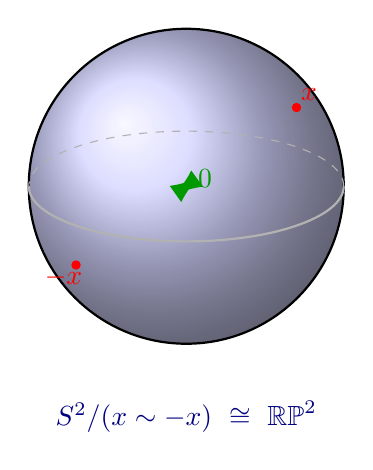
\begin{tikzpicture}[scale=2.0]
		% Sphere (as a circle)
		\shade[ball color=blue!20,opacity=0.9] (0,0) circle (1);
		\draw[thick] (0,0) circle (1);
		
		% "Equator" ellipse
		\draw[thick,gray!60] (-1,0) arc (180:360:1 and 0.35);
		\draw[dashed,gray!60] (1,0) arc (0:180:1 and 0.35);
		
		% Antipodal points x and -x
		\coordinate (X) at (0.7,0.5);
		\coordinate (Xm) at (-0.7,-0.5);
		
		\fill[red] (X) circle (0.03);
		\fill[red] (Xm) circle (0.03);
		
		% Labels (using calc instead of "of X")
		\node[red] at ($(X)+(0.08,0.08)$) {$x$};
		\node[red] at ($(Xm)+(-0.08,-0.08)$) {$-x$};
		
		% Origin and line through origin
		\coordinate (O) at (0,0);
		\draw[thick,green!60!black,->] (O) -- ($(X)!1.1!(O)$);
		\draw[thick,green!60!black,->] (O) -- ($(Xm)!1.1!(O)$);
		
		\node[green!60!black] at (0.12,0.05) {$0$};
		
		% Label of the quotient
		\node[blue!50!black,below] at (0,-1.3)
		{$S^2 / (x \sim -x)\ \cong\ \mathbb{RP}^2$};
	\end{tikzpicture}
	\caption{Sphere model of $\mathbb{RP}^2$: opposite points on $S^2$ are identified.}
	\label{fig:RP2_sphere_model}
\end{figure}

%=========================================================
% Figure 2: Disk model with antipodal boundary identification
%=========================================================
\begin{figure}[h]
	\centering
	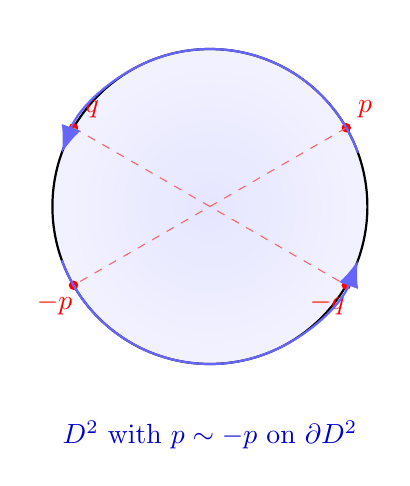
\begin{tikzpicture}[scale=2.0]
		% Disk
		\shade[inner color=blue!10,outer color=blue!5] (0,0) circle (1);
		\draw[thick] (0,0) circle (1);
		
		% A few sample boundary points and their antipodes
		\foreach \angle/\name in {30/p, 150/q} {
			\coordinate (\name) at (\angle:1);
			\coordinate (\name m) at (\angle+180:1);
			
			\fill[red] (\name) circle (0.03);
			\fill[red] (\name m) circle (0.03);
			
			% Labels via calc
			\node[red] at ($(\name)+(0.12,0.12)$) {$\name$};
			\node[red] at ($(\name m)+(-0.12,-0.12)$) {$-\name$};
			
			% Indicate identification by dashed chord
			\draw[red!60,dashed] (\name) -- (\name m);
		}
		
		% Arrows along boundary showing identification direction
		\draw[->,thick,blue!60] (20:1) arc (20:160:1);
		\draw[->,thick,blue!60] (200:1) arc (200:340:1);
		
		\node[blue!80!black,below] at (0,-1.3)
		{$D^2$ with $p \sim -p$ on $\partial D^2$};
	\end{tikzpicture}
	\caption{Disk model of $\mathbb{RP}^2$: the boundary circle has antipodal points identified.}
	\label{fig:RP2_disk_model}
\end{figure}

%=========================================================
% Figure 3: Fundamental polygon with edge word aa
%=========================================================
\begin{figure}[h]
	\centering
	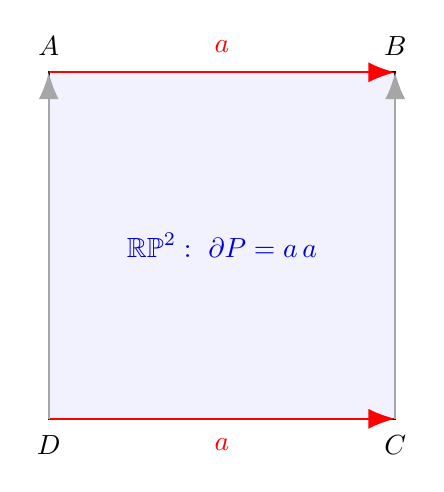
\begin{tikzpicture}[scale=2.2]
		% Square (fundamental polygon)
		\fill[blue!5] (-1,-1) rectangle (1,1);
		\draw[thick] (-1,-1) rectangle (1,1);
		
		% Label vertices (optional)
		\node[black] at (-1,1.15) {$A$};
		\node[black] at (1,1.15) {$B$};
		\node[black] at (1,-1.15) {$C$};
		\node[black] at (-1,-1.15) {$D$};
		
		% Top edge: a
		\draw[thick,red,->] (-1,1) -- (1,1);
		\node[red] at (0,1.15) {$a$};
		
		% Bottom edge: a (same orientation)
		\draw[thick,red,->] (-1,-1) -- (1,-1);
		\node[red] at (0,-1.15) {$a$};
		
		% Left/right edges (just gray guides)
		\draw[thick,gray!70,->] (-1,-1) -- (-1,1);
		\draw[thick,gray!70,->] (1,-1) -- (1,1);
		
		% Annotation
		\node[blue!80!black] at (0,0)
		{$\mathbb{RP}^2:\ \partial P = a\,a$};
		
	\end{tikzpicture}
	\caption{Fundamental polygon of $\mathbb{RP}^2$: a square with opposite edges identified in the same direction, giving the edge word $aa$.}
	\label{fig:RP2_fundamental_polygon}
\end{figure}

	
	\subsection{Sphere and Disk Models of $\mathbb{RP}^2$}
	
	A natural question is:
	
	\begin{quote}
		The disk model is 2-dimensional, but the sphere model lives in $\mathbb{R}^3$.
		How can both represent the same space $\mathbb{RP}^2$?
	\end{quote}
	
	We explain this carefully and geometrically.
	
	\subsubsection{$\mathbb{RP}^2$ is a 2-dimensional manifold}
	
	\begin{proposition}
		The real projective plane $\mathbb{RP}^2$ is a $2$-dimensional topological
		manifold.
	\end{proposition}
	
	\begin{proof}[Idea of proof]
		By definition
		\[
		\mathbb{RP}^2 = (\mathbb{R}^3 \setminus \{0\}) / \sim,
		\quad
		v \sim \lambda v \text{ for } \lambda \in \mathbb{R}\setminus\{0\},
		\]
		so each point of $\mathbb{RP}^2$ corresponds to a line through the origin in
		$\mathbb{R}^3$.  One can cover $\mathbb{RP}^2$ by affine charts of the form
		$\{[x:y:1]\}$, $\{[x:1:z]\}$, $\{[1:y:z]\}$, each homeomorphic to $\mathbb{R}^2$.
		These charts give it the structure of a $2$-dimensional manifold.
	\end{proof}
	
	Thus, any model of $\mathbb{RP}^2$ must be \emph{intrinsically} $2$-dimensional.
	
	\medskip
	
	The apparent discrepancy comes from the fact that one model is drawn in
	$\mathbb{R}^3$:
	
	\begin{itemize}
		\item The \emph{disk model} is manifestly 2-dimensional.
		\item The \emph{sphere model} uses a surface $S^2 \subset \mathbb{R}^3$, so we
		see it sitting in 3D, but the surface itself is 2-dimensional.
	\end{itemize}
	
	\subsubsection{Why does the sphere model start in $\mathbb{R}^3$?}
	
	Consider the model
	\[
	\mathbb{RP}^2 \cong S^2 / (x \sim -x),
	\]
	where $S^2 \subset \mathbb{R}^3$ is the unit sphere and we identify antipodal points.
	
	\begin{itemize}
		\item The sphere $S^2$ is a $2$-dimensional surface embedded in $\mathbb{R}^3$.
		\item The ambient space $\mathbb{R}^3$ is irrelevant for the intrinsic
		dimension; we are only using the surface of the sphere.
		\item The quotient $S^2/(x\sim -x)$ still has topological dimension $2$,
		since identifying points in pairs does not increase dimension.
	\end{itemize}
	
	Hence:
	
	\begin{quote}
		The sphere model of $\mathbb{RP}^2$ is \emph{2-dimensional}, not 3-dimensional;
		it is only \emph{drawn} in 3D.
	\end{quote}
	
	This is analogous to a rubber sheet: it is 2-dimensional even if you place it
	in a 3-dimensional room.
	
	\subsubsection{The disk model as a fundamental domain}
	
	The second standard model is
	\[
	\mathbb{RP}^2 \cong D^2 / (p \sim -p \text{ on } \partial D^2),
	\]
	where $D^2$ is the closed unit disk in $\mathbb{R}^2$ and points on the
	boundary circle are identified with their antipodes.
	
	Here:
	
	\begin{itemize}
		\item We start with a 2-dimensional disk $D^2$.
		\item We identify pairs of boundary points $p$ and $-p$.
		\item The resulting quotient is again a 2-dimensional surface.
	\end{itemize}
	
	This disk model is a \emph{fundamental domain} for the antipodal action on
	the sphere and is very convenient for:
	\begin{itemize}
		\item polygon gluings and classification of surfaces,
		\item describing the fundamental polygon,
		\item computing the fundamental group.
	\end{itemize}
	
	\subsubsection{Equivalence of the sphere and disk models}
	
	We now explain explicitly how the sphere model and the disk model give the
	same space.
	
	\begin{definition}[Upper hemisphere]
		Let
		\[
		S^2 = \{(x,y,z)\in\mathbb{R}^3 : x^2 + y^2 + z^2 = 1\},
		\]
		and define the upper hemisphere
		\[
		H = \{(x,y,z)\in S^2 : z \ge 0\}.
		\]
	\end{definition}
	
	We look at equivalence classes
	\[
	[x,y,z] = \{(x,y,z),(-x,-y,-z)\}.
	\]
	
	\paragraph{Step 1: From $S^2$ to the hemisphere.}
	\begin{itemize}
		\item If $z>0$, then in the class $\{(x,y,z),(-x,-y,-z)\}$, exactly one
		representative has $z>0$, and the other has $z<0$.
		Thus, each such class meets $H$ in exactly one point.
		\item If $z=0$ (the equator), then the class
		$\{(x,y,0),(-x,-y,0)\}$ lies entirely in the equator, and the two points are antipodal.
	\end{itemize}
	
	Hence each equivalence class in $S^2/(x\sim -x)$ has
	\begin{itemize}
		\item exactly one representative in the \emph{interior} of $H$ ($z>0$), and
		\item either one or two representatives on the equator, which are then identified.
	\end{itemize}
	
	Morally, $\mathbb{RP}^2$ is ``the upper hemisphere with antipodal identification on the equator.''
	
	\paragraph{Step 2: From hemisphere to disk.}
	
	Define
	\[
	\pi : H \longrightarrow D^2, 
	\qquad
	\pi(x,y,z) = (x,y),
	\]
	where
	\[
	D^2 = \{(u,v)\in\mathbb{R}^2 : u^2 + v^2 \le 1\}.
	\]
	
	This map is a homeomorphism:
	
	\begin{itemize}
		\item On $H$, we have $x^2 + y^2 + z^2 = 1$ with $z \ge 0$, so
		$x^2 + y^2 \le 1$. Thus $(x,y)\in D^2$.
		\item Given $(u,v)\in D^2$, we can recover
		\[
		z = \sqrt{1 - u^2 - v^2},
		\]
		so the inverse is
		\[
		\pi^{-1}(u,v) = (u,v,\sqrt{1-u^2-v^2}).
		\]
	\end{itemize}
	
	Therefore the upper hemisphere $H$ is homeomorphic to the disk $D^2$
	via $(x,y,z)\mapsto(x,y)$.
	
	\paragraph{Step 3: How the identification looks after flattening.}
	
	Combining the steps:
	
	\begin{enumerate}
		\item We start with the quotient by the antipodal map:
		\[
		(x,y,z) \sim (-x,-y,-z).
		\]
		\item We choose representatives with $z\ge 0$ (i.e.\ in $H$).
		\item We project to the disk via $\pi(x,y,z) = (x,y)$.
	\end{enumerate}
	
	\emph{Interior points.}  
	If $z>0$, the class
	\[
	\{(x,y,z),(-x,-y,-z)\}
	\]
	has a unique representative in $H$, namely $(x,y,z)$, which maps to
	$(x,y)$ with $x^2 + y^2 < 1$. No further identification occurs there.
	Thus, points in the interior of $D^2$ are not glued to anything else.
	
	\medskip
	
	\emph{Boundary points (equator / circle).}  
	If $(x,y,0)$ lies on the equator, then
	\[
	(x,y,0) \mapsto (x,y), \qquad (-x,-y,0) \mapsto (-x,-y),
	\]
	both on the unit circle. In $\mathbb{RP}^2$, these two points are
	identified since they are antipodal.
	
	Therefore, in the disk picture:
	
	\begin{quote}
		On the boundary circle $\partial D^2$, each point $(u,v)$ is identified 
		with its opposite point $(-u,-v)$.
	\end{quote}
	
	This is precisely the disk model
	\[
	\mathbb{RP}^2 \cong D^2 / \bigl( (u,v)\sim(-u,-v) \text{ on } \partial D^2 \bigr).
	\]
	
	\subsubsection{Summary and comparison of the models}
	
	We can summarize the relationship between the models in the following
	conceptual diagram:
	\[
	\begin{array}{ccc}
		S^2 & \xrightarrow{\ \text{quotient } x\sim -x\ } & \mathbb{RP}^2 \\[4pt]
		\Big\downarrow\text{restrict to } H & & \Big\uparrow\cong \\[4pt]
		H & \xrightarrow[\cong]{\ \pi\ } & D^2 / \bigl( p\sim -p \text{ on } \partial D^2 \bigr)
	\end{array}
	\]
	where $\pi(x,y,z) = (x,y)$.
	
	\begin{itemize}
		\item The \emph{sphere model} $S^2/(x\sim -x)$ emphasizes:
		\begin{itemize}
			\item compactness,
			\item non-orientability (the antipodal map reverses orientation),
			\item geometric and differential properties.
		\end{itemize}
		\item The \emph{disk model} $D^2/(p\sim -p)$ emphasizes:
		\begin{itemize}
			\item the fundamental polygon,
			\item the classification of surfaces,
			\item the edge word $aa$,
			\item computations of the fundamental group and other invariants.
		\end{itemize}
	\end{itemize}
	
	In both cases, the resulting space is a 2-dimensional manifold:
	
	\begin{quote}
		The dimension of $\mathbb{RP}^2$ is always $2$.  
		The sphere model uses a 2D surface embedded in $\mathbb{R}^3$; the ambient
		space plays no role in the intrinsic dimension.  
		The disk model works directly in $\mathbb{R}^2$.  
		The two models differ only in how we represent $\mathbb{RP}^2$, not in its
		dimension.
	\end{quote}
	
	
	\section*{Problem E2: Space of Lines and the M\"obius Band}
	
	Let $\Sigma$ be the set of all straight lines in $\mathbb{R}^2$.
	
	\begin{enumerate}
		\item[(a)] Prove that the set of straight lines in $\mathbb{R}^2$ admits the structure
		of a topological surface $\Sigma$ which is homeomorphic to a M\"obius band.
		(One possibility is to define an atlas with two charts by considering separately
		subsets of non-horizontal and non-vertical lines.)
		
		\item[(b)] Prove that the group of affine transformations
		\[
		\mathrm{Aff}(\mathbb{R}^2)
		= \{x \mapsto Ax + b \mid A \in GL(2,\mathbb{R}),\ b \in \mathbb{R}^2\}
		\]
		acts on $\Sigma$ by homeomorphisms.
		
		\item[(c)] Prove that there is no metric $d : \Sigma \times \Sigma \to \mathbb{R}_{\ge 0}$
		(in the sense of metric spaces) on $\Sigma$ which induces the given topology on $\Sigma$
		and for which $\mathrm{Aff}(\mathbb{R}^2)$ acts by isometries on $(\Sigma,d)$.
	\end{enumerate}
	
	\subsection*{Theory: Lines as a M\"obius Band}
	
	Every (unoriented) line $\ell \subset \mathbb{R}^2$ can be written as
	\[
	\ell = \{ x \in \mathbb{R}^2 : \langle x,n\rangle = r \}
	\]
	for some unit normal vector $n \in S^1$ and some signed distance $r \in \mathbb{R}$.
	If we replace $n$ by $-n$, the equation becomes
	$\langle x,-n\rangle = -r$, which describes the same line.  Thus the pairs
	$(n,r)$ and $(-n,-r)$ encode the same line, and we obtain a bijection
	\[
	\Sigma \;\cong\; (S^1\times\mathbb{R})/\!\sim,
	\qquad
	(n,r)\sim(-n,-r).
	\]
	
	If we precompose the $\mathbb{R}$--coordinate with any homeomorphism
	$\phi:\mathbb{R}\to(-1,1)$, we get an equivalent description
	\[
	\Sigma \;\cong\; (S^1\times(-1,1))/\!\sim,
	\qquad
	(\theta,t)\sim(\theta+\pi,-t),
	\]
	which is the standard construction of the M\"obius strip:
	take a rectangle $[0,2\pi]\times(-1,1)$ and identify $(0,t)\sim(2\pi,-t)$.
	
	\subsection*{Solution of (a)}
	
	Define
	\[
	F : S^1\times\mathbb{R} \longrightarrow \Sigma,
	\qquad
	F(n,r) = \{x\in\mathbb{R}^2 : \langle x,n\rangle = r\}.
	\]
	
	\begin{itemize}
		\item $F$ is surjective, since every line has some unit normal and signed distance.
		\item If $F(n,r) = F(m,s)$, then the corresponding line equations coincide,
		which forces $(m,s)=(n,r)$ or $(m,s)=(-n,-r)$.  Hence the fibers of $F$
		are exactly the equivalence classes of the relation $(n,r)\sim(-n,-r)$.
	\end{itemize}
	
	Thus $\Sigma$ is naturally homeomorphic to the quotient
	$(S^1\times\mathbb{R})/\!\sim$, and we put the quotient topology on $\Sigma$.
	Since $S^1\times\mathbb{R}$ is a $2$-dimensional manifold and the equivalence
	relation identifies points only in pairs along a free $\mathbb{Z}_2$-action,
	the quotient is again a $2$-dimensional manifold.
	
	Now choose a homeomorphism $\phi:\mathbb{R}\to(-1,1)$ and define
	\[
	\widetilde{F}:S^1\times(-1,1)\longrightarrow \Sigma,\qquad
	\widetilde{F}(n,t)=F\bigl(n,\phi^{-1}(t)\bigr).
	\]
	The same equivalence relation $(n,t)\sim(-n,-t)$ describes the same line,
	and hence
	\[
	\Sigma \;\cong\; (S^1\times(-1,1))/\bigl((n,t)\sim(-n,-t)\bigr).
	\]
	
	This quotient is homeomorphic to the standard M\"obius band, obtained
	from the rectangle $[0,2\pi]\times(-1,1)$ by identifying
	\[
	(0,t)\sim(2\pi,-t).
	\]
	Therefore $\Sigma$ is a topological surface homeomorphic to a M\"obius band.
	
	\begin{remark}[Alternative chart description]
		One may also construct $\Sigma$ from two charts:
		\begin{itemize}
			\item $\Sigma_1$: non-vertical lines, written as $y = mx + c$,
			identified with $(m,c)\in\mathbb{R}^2$.
			\item $\Sigma_2$: non-horizontal lines, written as $x = ny + d$,
			identified with $(n,d)\in\mathbb{R}^2$.
		\end{itemize}
		On the overlap (neither horizontal nor vertical), one has $m=\frac{1}{n}$
		and suitable relations between $(c,d)$, giving a nontrivial gluing.
		This atlas yields a surface whose transition functions realize the
		M\"obius twist.
	\end{remark}
	
	\subsection*{Solution of (b)}
	
	Given an affine transformation
	\[
	T(x) = A x + b, \quad A\in GL(2,\mathbb{R}),\ b\in\mathbb{R}^2,
	\]
	and a line $\ell\subset\mathbb{R}^2$, define
	\[
	T\cdot \ell := T(\ell) = \{T(x) : x\in\ell\}.
	\]
	
	Because $T$ is a bijective affine map, $T(\ell)$ is a straight line, so
	$T\cdot\ell\in\Sigma$.  If $\ell_1=\ell_2$ then $T(\ell_1)=T(\ell_2)$, so the
	operation is well defined, and 
	\[
	(T_1T_2)\cdot\ell = T_1\bigl(T_2(\ell)\bigr),
	\]
	so we indeed have a group action of $\mathrm{Aff}(\mathbb{R}^2)$ on $\Sigma$.
	
	Each affine map $T$ is a homeomorphism of $\mathbb{R}^2$ with inverse $T^{-1}$,
	hence it induces a homeomorphism of $\Sigma$:
	\[
	\Sigma\to\Sigma,\quad \ell\mapsto T(\ell),
	\]
	with inverse $\ell\mapsto T^{-1}(\ell)$.  Therefore
	$\mathrm{Aff}(\mathbb{R}^2)$ acts on $\Sigma$ by homeomorphisms.
	
	\subsection*{Solution of (c)}
	
	Suppose, for a contradiction, that there exists a metric
	$d:\Sigma\times\Sigma\to\mathbb{R}_{\ge 0}$ such that
	\begin{enumerate}
		\item $d$ induces the given topology on $\Sigma$;
		\item for all $T\in\mathrm{Aff}(\mathbb{R}^2)$ and all $\ell_1,\ell_2\in\Sigma$,
		\[
		d\bigl(T(\ell_1),T(\ell_2)\bigr) = d(\ell_1,\ell_2).
		\]
	\end{enumerate}
	
	\paragraph{Step 1: Distance depends only on angle.}
	Let $\ell_1,\ell_2$ be distinct non-parallel lines making angle $\theta\in(0,\pi)$.
	There exists $T\in\mathrm{Aff}(\mathbb{R}^2)$ such that
	\[
	T(\ell_1) = L_1,\qquad T(\ell_2) = L_2,
	\]
	where $L_1,L_2$ are, for example, two lines through the origin meeting at angle
	$\theta$.  Any two ordered pairs of lines having the same angle are related by an
	element of $GL(2,\mathbb{R})$, and hence by an affine transformation.
	
	Therefore there is a function $f:(0,\pi)\to[0,\infty)$ such that
	\[
	d(\ell_1,\ell_2) = f(\theta)
	\]
	for any pair of intersecting lines with angle $\theta$ between them.
	
	Similarly, for $\theta=0$ (distinct parallel lines), any two ordered pairs of
	distinct parallel lines are related by an affine transformation, so all such
	pairs have the same distance, say $f(0)>0$.
	
	Thus for all pairs of distinct lines, the distance depends only on the angle
	between them.
	
	\paragraph{Step 2: Continuity and parallel lines.}
	
	Since $\Sigma$ is a M\"obius band with the quotient topology, it is a connected
	$2$-dimensional manifold.  In particular, the metric $d$ must be compatible
	with the manifold topology, so $d$ is continuous in its arguments.
	
	Fix a line $\ell$.  Consider a sequence of lines $\ell_k$ that intersect $\ell$
	in the origin and whose angle $\theta_k$ with $\ell$ satisfies $\theta_k\to 0$.
	In the M\"obius-band topology, we have $\ell_k\to\ell$.  Hence, by continuity,
	\[
	d(\ell_k,\ell) \longrightarrow d(\ell,\ell)=0.
	\]
	But by the angle dependence,
	\[
	d(\ell_k,\ell) = f(\theta_k),
	\]
	so
	\[
	f(\theta_k)\longrightarrow 0
	\quad\Rightarrow\quad
	\lim_{\theta\to 0^+} f(\theta) = 0.
	\]
	
	Now let $\ell_1,\ell_2$ be two distinct parallel lines.  Their angle is $0$, so
	\[
	d(\ell_1,\ell_2) = f(0).
	\]
	By the affine invariance, $f(0)$ is the same positive constant for all pairs
	of distinct parallel lines.
	
	Choose lines $\ell_{2,k}$ intersecting $\ell_1$ whose angle with $\ell_1$ is
	$\theta_k\to 0$ and such that $\ell_{2,k}\to\ell_2$ in $\Sigma$.  Then
	\[
	d(\ell_1,\ell_{2,k}) \to d(\ell_1,\ell_2) = f(0).
	\]
	On the other hand, for each $k$,
	\[
	d(\ell_1,\ell_{2,k}) = f(\theta_k) \longrightarrow 0.
	\]
	Thus $f(0)=0$ and $f(0)>0$ simultaneously, a contradiction.
	
	Therefore no metric $d$ on $\Sigma$ can both induce the given topology and
	make the action of $\mathrm{Aff}(\mathbb{R}^2)$ isometric.
	\hfill $\square$
	
	\begin{figure}[h]
		\centering
		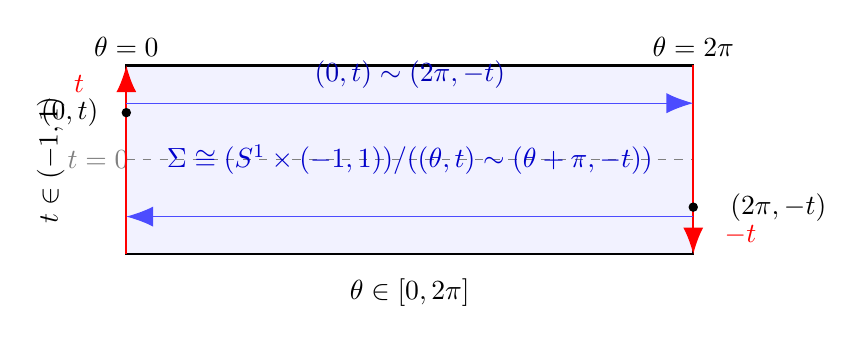
\begin{tikzpicture}[scale=1.2]
			
			% Rectangle representing S^1 x (-1,1)
			\fill[blue!5] (0,-1) rectangle (6,1);
			\draw[thick] (0,-1) rectangle (6,1);
			
			% Horizontal axis t = 0
			\draw[dashed,gray] (0,0) -- (6,0);
			\node[gray] at (-0.3,0) {$t=0$};
			
			% Label theta at bottom
			\node at (3,-1.4) {$\theta \in [0,2\pi]$};
			\node[rotate=90] at (-0.8,0) {$t \in (-1,1)$};
			
			% Left edge labels (theta = 0)
			\node at (0,1.2) {$\theta=0$};
			\draw[thick,red,->] (0,-1) -- (0,1);
			\node[red] at (-0.5,0.8) {$t$};
			
			% Right edge labels (theta = 2pi)
			\node at (6,1.2) {$\theta = 2\pi$};
			\draw[thick,red,->] (6,1) -- (6,-1);
			\node[red] at (6.5,-0.8) {$-t$};
			
			% Arrows showing identification
			\draw[blue!70,->] (0,0.6) to[out=0,in=180] (6,0.6);
			\draw[blue!70,->] (6,-0.6) to[out=180,in=0] (0,-0.6);
			
			\node[blue!70!black] at (3,0.9)
			{$(0,t)\sim(2\pi,-t)$};
			
			% A few sample points and their images
			\fill[black] (0,0.5) circle (0.05);
			\fill[black] (6,-0.5) circle (0.05);
			\node[black] at (-0.6,0.5) {$(0,t)$};
			\node[black] at (6.9,-0.5) {$(2\pi,-t)$};
			
			% Caption inside
			\node[blue!80!black] at (3,0)
			{$\Sigma \cong (S^1\times(-1,1))/((\theta,t)\sim(\theta+\pi,-t))$};
			
		\end{tikzpicture}
		\caption{Normal--distance parametrisation of lines:
			the quotient of $[0,2\pi]\times(-1,1)$ by $(0,t)\sim(2\pi,-t)$
			is a M\"obius band, homeomorphic to $\Sigma$.}
		\label{fig:mobius_normal_distance}
	\end{figure}
	
	\paragraph{Description of the quotient.}
	The rectangle $[0,2\pi]\times(-1,1)$ parametrises all straight lines in
	$\mathbb{R}^2$ as follows:
	for $\theta\in[0,2\pi]$ define $n(\theta)=(\cos\theta,\sin\theta)$, and let
	$t\in(-1,1)$ denote a (scaled) signed distance of a line from the origin.
	Each pair $(\theta,t)$ determines the line
	\[
	\ell_{\theta,t}=\{x\in\mathbb{R}^2:\langle x,n(\theta)\rangle=t\}.
	\]
	
	Since the unit normals $n(\theta)$ and $n(\theta+\pi)$ differ by a sign,
	the pairs $(\theta,t)$ and $(\theta+\pi,-t)$ encode the same line.
	In terms of the rectangle parametrisation this produces the identification
	\[
	(0,t)\sim(2\pi,-t), \qquad t\in(-1,1).
	\]
	
	The quotient space
	\[
	\bigl([0,2\pi]\times(-1,1)\bigr)\big/\bigl((0,t)\sim(2\pi,-t)\bigr)
	\]
	is therefore obtained by gluing the two vertical edges of the rectangle with
	a half–twist.  This is precisely the construction of the M\"obius band.
	Hence the space $\Sigma$ of all straight lines in $\mathbb{R}^2$ is
	homeomorphic to a M\"obius band.
	
	\section*{Normals, the Rectangle Model, and the M\"obius Gluing}
	
	\subsection*{The meaning of $(\theta,t)$}
	
	The rectangle $[0,2\pi]\times(-1,1)$ is a \emph{parameter space} for the set
	$\Sigma$ of all straight lines in $\mathbb{R}^2$.  
	A point
	\[
	(\theta,t)\in[0,2\pi]\times(-1,1)
	\]
	is not a point of the plane, but an encoding of a line.
	
	\paragraph{The coordinate $\theta$.}
	For each $\theta\in[0,2\pi]$ define the unit vector
	\[
	n(\theta) = (\cos\theta,\sin\theta)\in S^{1}.
	\]
	Thus $\theta$ parametrises the unit circle $S^1$,
	``unwrapped'' to the interval $[0,2\pi]$.
	This is the \emph{normal direction} of the line.
	
	\paragraph{The coordinate $t$.}
	The real number $t\in(-1,1)$ (obtained from the signed distance $r\in\mathbb{R}$
	via a homeomorphism $\phi:\mathbb{R}\to(-1,1)$) is the
	\emph{offset} of the line from the origin in the normal direction.
	
	\paragraph{Reconstruction of a line.}
	The point $(\theta,t)$ corresponds to the line
	\[
	\ell_{\theta,t}
	= \{x\in\mathbb{R}^2 : \langle x,n(\theta)\rangle = t\}.
	\]
	
	\subsection*{Why the M\"obius gluing occurs}
	
	The normals $n(\theta)$ and $n(\theta+\pi)$ point in opposite directions, so
	\[
	\langle x,n(\theta)\rangle = t
	\quad\Longleftrightarrow\quad
	\langle x,n(\theta+\pi)\rangle = -t.
	\]
	Thus $(\theta,t)$ and $(\theta+\pi,-t)$ encode the \emph{same} geometric line.
	In particular,
	\[
	(0,t)\sim(2\pi,-t),\qquad t\in(-1,1).
	\]
	Gluing the two vertical edges of the rectangle by $(0,t)\sim(2\pi,-t)$ produces
	the standard M\"obius band, which is therefore homeomorphic to $\Sigma$.
	
		\clearpage
	
	\bigskip
	\hrule
	\bigskip
	
	\subsection*{Diagram 1: Unit circle unwrapped to the $\theta$--axis}
	
	\begin{figure}[h]
		\centering
		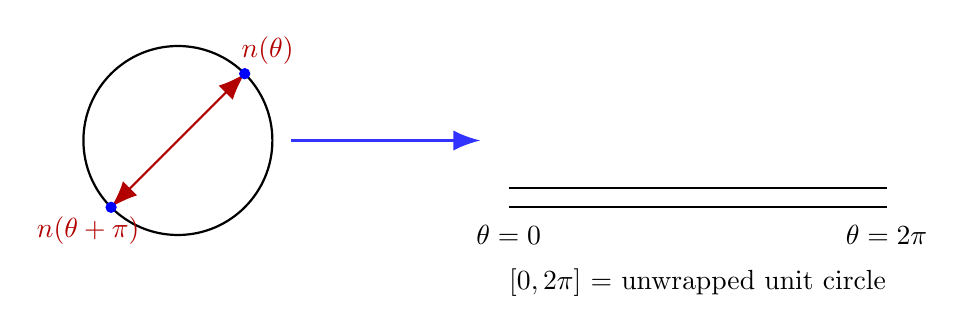
\begin{tikzpicture}[scale=1.2]
			
			% Circle
			\draw[thick] (0,0) circle (1);
			
			% Radius arrows & labels
			\draw[->,red!70!black,thick] (0,0) -- (0.707,0.707);
			\draw[->,red!70!black,thick] (0,0) -- (-0.707,-0.707);
			
			\node[red!70!black] at (0.95,0.95) {$n(\theta)$};
			\node[red!70!black] at (-0.95,-0.95) {$n(\theta+\pi)$};
			
			% Points
			\fill[blue] (0.707,0.707) circle (0.06);
			\fill[blue] (-0.707,-0.707) circle (0.06);
			
			% Arrow showing unwrap
			\draw[thick,->,blue!80] (1.2,0) -- (3.2,0);
			
			% Interval
			\draw[thick] (3.5,-0.5) -- (7.5,-0.5);
			\draw[thick] (3.5,-0.7) -- (7.5,-0.7);
			
			\node at (3.5,-1) {$\theta=0$};
			\node at (7.5,-1) {$\theta=2\pi$};
			
			\node at (5.5,-1.5) {$[0,2\pi]$ = unwrapped unit circle};
			
		\end{tikzpicture}
		\caption{The normal direction $n(\theta)$ lies on $S^1$, which is represented in the rectangle model by unwrapping $S^1$ to $[0,2\pi]$.}
	\end{figure}
	
	\bigskip
	\hrule
	\bigskip
	

	
	\subsection*{Diagram 2: How a line in $\mathbb{R}^2$ maps to $(\theta,t)$}
	
\begin{figure}[h]
	\centering
	\begin{tikzpicture}[scale=1.3]
		
		% Axes
		\draw[->] (-2,0) -- (2,0) node[right] {$x$};
		\draw[->] (0,-2) -- (0,2) node[above] {$y$};
		
		% Parameters
		\def\theta{55} % angle of normal
		\def\t{0.7}    % offset t
		
		% Normal vector n(theta)
		\draw[->,red!70!black,thick] (0,0) -- ({cos(\theta)},{sin(\theta)})
		node[red!70!black,anchor=west] {$n(\theta)$};
		
		% The line: point (1,t) and direction perpendicular to normal
		% Tangent direction is rotated by 90 degrees
		\draw[thick,blue] 
		({1 - 2*sin(\theta)},{\t + 2*cos(\theta)})
		--
		({1 + 2*sin(\theta)},{\t - 2*cos(\theta)});
		
		% Mark point (1,t)
		\fill (1,\t) circle (0.06);
		\node[anchor=west] at (1.1,\t) {$(1,t)$};
		
		% Label t distance (dashed projection)
		\draw[dashed] (0,0) -- ( {cos(\theta)*\t} , {sin(\theta)*\t} );
		\node at ( {cos(\theta)*\t/2} , {sin(\theta)*\t/2} ) {$t$};
		
		% Mapping arrow
		\draw[->,thick,blue!80] (2.2,0) -- (4.2,0);
		
		% Rectangle + point for (\theta,t)
		\draw[blue!40,dashed] (4.8,-1) rectangle (6.8,1);
		\fill (5.8,0.3) circle (0.06);
		\node[right] at (5.85,0.3) {$(\theta,t)$};
		
		\node at (5.8,-1.3) {$[0,2\pi]\times(-1,1)$};
		
	\end{tikzpicture}
	\caption{A line at signed distance $t$ from the origin with normal direction $n(\theta)$ corresponds to the point $(\theta,t)$ in the parameter rectangle.}
\end{figure}

	\subsection*{Scaling of the distance coordinate and relation to slope}
	
	\paragraph{Rescaling the distance.}
	A geometric line in $\mathbb{R}^2$ can always be written in \emph{normal form}
	\[
	\ell_{\theta,r}
	= \{(x,y)\in\mathbb{R}^2 : x\cos\theta + y\sin\theta = r\},
	\qquad \theta\in[0,2\pi),\ r\in\mathbb{R}.
	\]
	Here $r$ is the signed distance of the line from the origin in the direction
	of the unit normal vector $n(\theta)=(\cos\theta,\sin\theta)$.
	
	In order to obtain a bounded parameter domain (the rectangle
	$[0,2\pi]\times(-1,1)$), we replace $r\in\mathbb{R}$ by a new coordinate
	\[
	t = \phi(r) \in (-1,1),
	\]
	where $\phi:\mathbb{R}\to(-1,1)$ is any homeomorphism (for example,
	$\displaystyle \phi(r)=\tfrac{2}{\pi}\arctan r$ or $\phi(r)=\tanh r$).
	Thus $t$ is merely a \emph{rescaled} distance coordinate; very large values
	$|r|\to\infty$ correspond to $t\to\pm 1$.
	
	Consequently, a point $(\theta,t)\in[0,2\pi]\times(-1,1)$ encodes the same
	geometric line as $(\theta,r)$ with $r=\phi^{-1}(t)$.
	
	\paragraph{Relation between the slope and the normal angle.}
	Writing a line in slope--intercept form
	\[
	y = ax + b,
	\]
	the slope $a$ is the tangent of the angle $\varphi$ that the line makes with
	the positive $x$--axis:
	\[
	a = \tan\varphi.
	\]
	
	In the normal-distance parametrisation, the direction of the line is
	orthogonal to the normal $n(\theta)$, so the angle of the line is
	\[
	\varphi = \theta - \frac{\pi}{2}.
	\]
	Hence
	\[
	a = \tan\!\Bigl(\theta - \frac{\pi}{2}\Bigr)
	= -\cot\theta.
	\]
	
	\paragraph{Converting between normal form and slope--intercept form.}
	Starting from the normal equation
	\[
	x\cos\theta + y\sin\theta = r,
	\]
	and solving for $y$ gives
	\[
	y
	= -\frac{\cos\theta}{\sin\theta}\,x
	+ \frac{r}{\sin\theta}
	= -\cot\theta\,x + r\,\csc\theta.
	\]
	Thus the parameters are related by
	\[
	a = -\cot\theta,
	\qquad
	b = r\,\csc\theta.
	\]
	
	Conversely, given a slope $a\in\mathbb{R}$, we may recover the normal angle
	$\theta$ by
	\[
	\theta = \arctan\!\left(-\frac{1}{a}\right),
	\qquad
	\text{(mod $\pi$ since $n(\theta)$ and $n(\theta+\pi)$ define the same line).}
	\]
	The signed distance $r$ can then be computed from any point $(x_0,y_0)$ on the
	line by
	\[
	r = x_0\cos\theta + y_0\sin\theta.
	\]
	
	\medskip
	In summary:
	\[
	(\theta,r)\quad\leftrightarrow\quad(a,b)
	\]
	are related by the formulas
	\[
	a=-\cot\theta,\qquad b=r\,\csc\theta,
	\]
	and the coordinate $t\in(-1,1)$ is simply a bounded rescaling of the true
	distance $r\in\mathbb{R}$.
	
	
\section*{E3: Unordered Pairs on a Circle and Inscribed Rectangles}

\subsection*{Problem}

Let $S^{1}\subset\mathbb{R}^{2}$ be the unit circle and let
$X$ denote the set of unordered pairs $\{p,q\}$ of points on $S^{1}$.

\begin{enumerate}[label=\textnormal{(\alph*)}]
	\item Explain why $X$ is naturally a quotient space of the torus
	$T^{2}=S^{1}\times S^{1}$.  By considering $T^{2}$ as a quotient space
	of a square, or otherwise, show that
	\[
	X \cong \mathbb{RP}^{2}\setminus\overline{D},
	\]
	the complement of a closed disc in $\mathbb{RP}^{2}$.
	
	\item Let $D=\{z\in\mathbb{C}:|z|\le 1\}$ be a closed disc and let
	$\phi:D\to\mathbb{R}^{2}$ be a continuous injection with boundary
	$C=\phi(S^{1})\subset\mathbb{R}^{2}$.  Define
	\[
	f:C\times C\to\mathbb{R}^{3},\qquad
	(u,v)\longmapsto \left(\frac{u+v}{2},\,|u-v|\right)\in\mathbb{R}^{2}\times\mathbb{R}.
	\]
	Show that $f$ defines a map on $X$, which extends to a continuous map
	$\hat f:\mathbb{RP}^{2}\to\mathbb{R}^{3}$.
	
	\item Using without proof that a compact non-orientable topological surface
	cannot be continuously embedded in $\mathbb{R}^{3}$, deduce that $C$
	bounds an \emph{inscribed rectangle}, i.e.\ there exist four pairwise
	distinct points on $C$ which form the vertices of a rectangle in $\mathbb{R}^{2}$
	(the rectangle need not be contained in $\phi(D)$).
\end{enumerate}

\begin{figure}[h!]
	\centering
	
\includegraphics[width=0.72\textwidth]{e3.png}
	\caption{Two examples of inscribed rectangles on a Jordan curve $C$.
		On the left: a nearly convex curve containing a rectangle.
		On the right: a wild, nonconvex curve still containing a rectangle,
		illustrating the conclusion of part (c).}
	\label{fig:e3-rectangles}
\end{figure}


\subsubsection*{Theory}

\paragraph{Configuration space.}
The torus $T^{2}=S^{1}\times S^{1}$ parametrises ordered pairs $(p,q)$ of
points on $S^{1}$.  The set of unordered pairs is the symmetric product
\[
X = \operatorname{Sym}^{2}(S^{1})
= (S^{1}\times S^{1})/\tau,
\]
where $\tau:T^{2}\to T^{2}$ is the involution $\tau(p,q)=(q,p)$.

The diagonal
\[
\Delta=\{(p,p)\in T^{2}:p\in S^{1}\}
\]
consists of pairs with $p=q$ and is precisely the fixed point set of $\tau$.
On $T^{2}\setminus\Delta$ the action of $\tau$ is free, and each orbit has
two points.

\paragraph{Quotient and relation to $\mathbb{RP}^{2}$.}
Model $T^{2}$ as the unit square with opposite sides identified.
The involution $\tau$ is reflection across the main diagonal.  The quotient
of the square by this reflection identifies the two triangular halves and
produces a 2--cell whose boundary is the image of the diagonal.  Attaching the
edges according to the torus identifications yields $\mathbb{RP}^{2}$, with the
image of $\Delta$ forming a simple closed curve.  Removing a small open disc
around that curve corresponds to discarding a neighbourhood of the diagonal,
and the resulting space is homeomorphic to $X$.  Thus
\[
X \cong \mathbb{RP}^{2}\setminus\overline{D}.
\]

\paragraph{The map $f$.}
For $u,v\in C\subset\mathbb{R}^{2}$,
\[
f(u,v)=\left(\frac{u+v}{2},\,|u-v|\right)
\]
encodes the midpoint and length of the chord joining $u$ and $v$.
Since $f(u,v)=f(v,u)$, the value of $f$ depends only on the unordered pair
$\{u,v\}$.

Degenerate pairs with $u=v$ correspond to the diagonal $\Delta$.
For such pairs,
\[
f(u,u)=(u,0),
\]
and as $(u,v)\to(u,u)$, the midpoint tends to $u$ and the distance to $0$.
Thus $f$ extends continuously across the diagonal, and via the identification
$X\cong\mathbb{RP}^{2}\setminus\overline{D}$ further extends to a continuous
map $\hat f:\mathbb{RP}^{2}\to\mathbb{R}^{3}$.

\paragraph{Rectangles and collisions of $f$.}
If $u_{1},u_{2},u_{3},u_{4}\in C$ are vertices of a rectangle, then the opposite
vertices form two unordered pairs $\{u_{1},u_{3}\}$ and $\{u_{2},u_{4}\}$
whose diagonals have the same midpoint and the same length.  Equivalently,
\[
f(u_{1},u_{3}) = f(u_{2},u_{4}).
\]
Thus distinct unordered pairs with the same image under $f$ correspond exactly
to inscribed rectangles.  If no such rectangle exists, then the induced map
$\bar f:X\to\mathbb{R}^{3}$ is injective; together with compactness this would
produce an embedding of $\mathbb{RP}^{2}$ into $\mathbb{R}^{3}$, contradicting
the known theorem on non-orientable surfaces.
	
	\subsection*{(a) Description of $X$ and its topology}
	
	Let
	\[
	X=\{\{p,q\}\subset S^{1} : p,q\in S^{1}\}
	\]
	be the set of unordered pairs of points on the circle.  The torus
	$T^{2}=S^{1}\times S^{1}$ parametrises ordered pairs $(p,q)$.
	Define the involution
	\[
	\tau : T^{2}\longrightarrow T^{2},\qquad \tau(p,q)=(q,p).
	\]
	Then $\tau^{2}=\mathrm{id}$ and two ordered pairs determine the same unordered
	pair iff they lie in the same $\tau$--orbit.  Hence
	\[
	X = T^{2}/\tau .
	\]
	
	Let $\Delta=\{(p,p):p\in S^{1}\}$ be the diagonal of $T^{2}$.  This is precisely
	the fixed point set of $\tau$.  On $T^{2}\setminus\Delta$ the involution acts
	freely, and the quotient identifies each point above the diagonal with its
	mirror image below it.
	
	Represent $T^{2}$ as a square with opposite edges identified.  The involution
	$\tau$ becomes reflection across the diagonal of the square.  The quotient of
	the square by reflection identifies the two triangular halves, producing a
	2--cell whose boundary is the image of $\Delta$.
	
	This quotient space is homeomorphic to the projective plane with an open disc
	removed.  Therefore
	\[
	X \cong T^{2}/\tau \cong \mathbb{RP}^{2}\setminus \overline{D},
	\]
	as required.
	
\subsection*{Solutions}

\subsubsection*{(a) $X$ as a quotient of the torus and as
	$\mathbb{RP}^{2}\setminus \overline{D}$}

\paragraph{Quotient of the torus.}
Let $T^{2}=S^{1}\times S^{1}$ and define the involution
\[
\tau:T^{2}\longrightarrow T^{2},\qquad \tau(p,q)=(q,p).
\]
The $\tau$–orbits are:
\begin{itemize}
	\item singletons $(p,p)$ on the diagonal $\Delta=\{(p,p):p\in S^{1}\}$;
	\item pairs $(p,q)\leftrightarrow(q,p)$ when $p\neq q$.
\end{itemize}
Thus unordered pairs $\{p,q\}$ are precisely the $\tau$–orbits, and with the
quotient topology we obtain
\[
X \;=\; T^{2}/\tau.
\]

\paragraph{From the torus to $\mathbb{RP}^{2}\setminus\overline{D}$.}
Model $T^{2}$ as the unit square with opposite sides identified.
The map $\tau$ is reflection across the main diagonal of the square.
The quotient of the square by this reflection identifies the two triangular
halves and yields a $2$–cell whose boundary is the image of the diagonal.
After performing the edge identifications one obtains $\mathbb{RP}^{2}$.

Removing a small open disc around that boundary corresponds to discarding a
neighbourhood of the diagonal in $T^{2}$; the remaining space is exactly $X$.
Hence
\[
X \;\cong\; \mathbb{RP}^{2}\setminus\overline{D}.
\]

%---------------------------------------------------------------------%

\subsubsection*{(b) $f$ factors through $X$ and extends to
	$\hat f:\mathbb{RP}^{2}\to\mathbb{R}^{3}$}

\paragraph{Symmetry.}
For $u,v\in C$ we have
\[
f(u,v)
=\left(\frac{u+v}{2},\,|u-v|\right)
=\left(\frac{v+u}{2},\,|v-u|\right)
=f(v,u).
\]
Thus $f$ is constant on unordered pairs $\{u,v\}$ and therefore induces a
well-defined map
\[
\bar f:X\longrightarrow\mathbb{R}^{3},\qquad
\bar f(\{u,v\})=f(u,v).
\]
Since $f$ is continuous and the quotient map $C\times C\to X$ is open,
$\bar f$ is continuous.

\paragraph{Extension over the diagonal / missing disc.}
The diagonal $\Delta\subset S^{1}\times S^{1}$ corresponds to pairs with
$u=v$.  For such pairs,
\[
f(u,u)
=\left(\frac{u+u}{2},\,|u-u|\right)
=(u,0).
\]
As $(u,v)\to(u,u)$, the midpoint tends to $u$ and the distance tends to $0$,
so $f$ extends continuously along the diagonal.

In the quotient picture $X\cong\mathbb{RP}^{2}\setminus\overline{D}$, the
diagonal becomes the missing disc; filling it in corresponds to allowing
$u=v$.  Hence $f$ extends to a continuous map
\[
\hat f:\mathbb{RP}^{2}\longrightarrow\mathbb{R}^{3}
\]
whose restriction to $X\cong\mathbb{RP}^{2}\setminus\overline{D}$ is $\bar f$.

%---------------------------------------------------------------------%

\subsubsection*{(c) Existence of an inscribed rectangle}

Assume for contradiction that $C$ bounds no inscribed rectangle.

\paragraph{Injectivity of $\bar f$.}
Suppose
\[
\bar f(\{u,v\})=\bar f(\{u',v'\})
\]
for some $u,v,u',v'\in C$.  Then
\[
\frac{u+v}{2}=\frac{u'+v'}{2},\qquad
|u-v|=|u'-v'|.
\]
Thus the chords $uv$ and $u'v'$ have the same midpoint and the same length.
This is exactly the condition for the quadrilateral $u,v,u',v'$ to have
equal-length diagonals with common midpoint, i.e.\ to be a rectangle
(possibly degenerate if points coincide).  Our assumption that there is no
non-degenerate rectangle with vertices on $C$ therefore forces
\[
\{u,v\}=\{u',v'\}.
\]
Hence $\bar f$ is injective on $X$.

\paragraph{Embedding of $\mathbb{RP}^{2}$.}
The extension $\hat f:\mathbb{RP}^{2}\to\mathbb{R}^{3}$ is continuous.
On the dense subset $X\subset\mathbb{RP}^{2}$ it is injective; by continuity
and compactness, $\hat f$ is in fact injective on all of $\mathbb{RP}^{2}$.

A continuous injective map from a compact space into a Hausdorff space is a
homeomorphism onto its image, so $\hat f$ is a topological embedding of
$\mathbb{RP}^{2}$ into $\mathbb{R}^{3}$.

\paragraph{Contradiction.}
This contradicts the given fact that a compact non-orientable surface cannot
be embedded in $\mathbb{R}^{3}$.  Therefore our assumption was false, and
there must exist at least one inscribed rectangle on $C$.
\qedhere

	
	\subsubsection*{Torus as a Quotient of the Square}
	
	Let $Q=[0,1]\times[0,1]$ be the unit square.  
	Define an equivalence relation $\sim$ on $Q$ by
	\[
	(0,y)\sim(1,y),\qquad (x,0)\sim(x,1),
	\]
	for all $x,y\in[0,1]$.  
	That is, the left and right edges are identified pointwise, and likewise the
	bottom and top edges.
	
	The quotient space
	\[
	T^{2} \;=\; Q /{\sim}
	\]
	is the standard torus.  Gluing the left and right edges of $Q$ produces a
	cylinder, and gluing the two boundary circles of the cylinder produces a torus.
	
	Thus the torus admits the classical description
	\[
	T^{2} \;\cong\; [0,1]^{2}/\!\sim.
	\]
	
	
	\begin{figure}[h!]
		\centering
		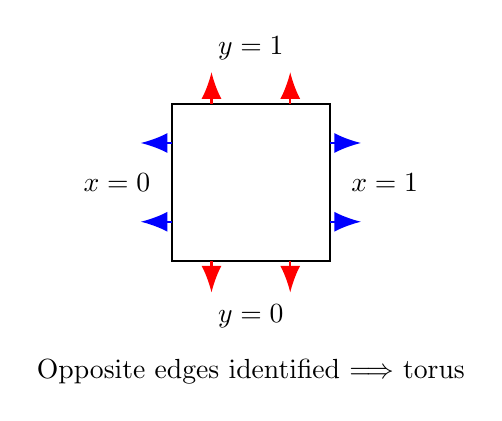
\begin{tikzpicture}[scale=2]
			
			% square
			\draw[thick] (0,0) rectangle (1,1);
			
			% arrows for horizontal identification
			\draw[->,blue,thick] (0,0.25) -- (-0.2,0.25);
			\draw[->,blue,thick] (1,0.25) -- (1.2,0.25);
			\draw[->,blue,thick] (0,0.75) -- (-0.2,0.75);
			\draw[->,blue,thick] (1,0.75) -- (1.2,0.75);
			
			% arrows for vertical identification
			\draw[->,red,thick] (0.25,0) -- (0.25,-0.2);
			\draw[->,red,thick] (0.75,0) -- (0.75,-0.2);
			\draw[->,red,thick] (0.25,1) -- (0.25,1.2);
			\draw[->,red,thick] (0.75,1) -- (0.75,1.2);
			
			% labels
			\node at (-0.35,0.5) {$x=0$};
			\node at (1.35,0.5) {$x=1$};
			\node at (0.5,-0.35) {$y=0$};
			\node at (0.5,1.35) {$y=1$};
			
			\node at (0.5,-0.7) {Opposite edges identified $\Longrightarrow$ torus};
			
		\end{tikzpicture}
		\caption{The torus $T^{2}$ as the quotient of a square with opposite edges
			identified.}
	\end{figure}
	
	
	\begin{figure}[h]
		\centering
		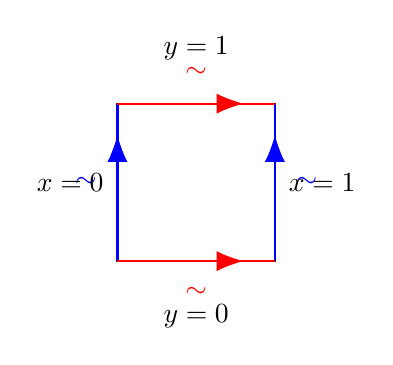
\begin{tikzpicture}[scale=2]
			
			% Square
			\draw[thick] (0,0) rectangle (1,1);
			
			% Left/right edges (blue, oriented upwards)
			\draw[thick,blue] (0,0) -- (0,1);
			\draw[thick,blue] (1,0) -- (1,1);
			\draw[blue,->] (0,0.2) -- (0,0.8);
			\draw[blue,->] (1,0.2) -- (1,0.8);
			\node[blue] at (-0.2,0.5) {$\sim$};
			\node[blue] at ( 1.2,0.5) {$\sim$};
			
			% Bottom/top edges (red, oriented to the right)
			\draw[thick,red] (0,0) -- (1,0);
			\draw[thick,red] (0,1) -- (1,1);
			\draw[red,->] (0.2,0) -- (0.8,0);
			\draw[red,->] (0.2,1) -- (0.8,1);
			\node[red]  at (0.5,-0.2) {$\sim$};
			\node[red]  at (0.5, 1.2) {$\sim$};
			
			% Labels
			\node at (-0.3,0.5) {$x=0$};
			\node at ( 1.3,0.5) {$x=1$};
			\node at (0.5,-0.35) {$y=0$};
			\node at (0.5, 1.35) {$y=1$};
			
		\end{tikzpicture}
		\caption{The torus $T^{2}$ as $[0,1]^{2}$ with opposite edges identified
			orientation–preservingly (blue: vertical edges, red: horizontal edges).}
		\label{fig:torus-square}
	\end{figure}
	
	\begin{figure}[h]
		\centering
		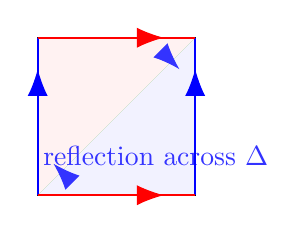
\begin{tikzpicture}[scale=2]
			
			% Square
			\fill[gray!5] (0,0) rectangle (1,1);
			\draw[thick] (0,0) rectangle (1,1);
			
			% Diagonal (reflection axis)
			\draw[thick,green!60!black] (0,0) -- (1,1);
			\node[green!60!black,anchor=south west] at (0.05,0.05) {$\Delta$};
			
			% Shade the two triangles lightly
			\fill[blue!5]  (0,0) -- (1,0) -- (1,1) -- cycle;
			\fill[red!5]   (0,0) -- (0,1) -- (1,1) -- cycle;
			
			% Arrows indicating reflection
			\draw[->,blue!80] (0.2,0.1) -- (0.1,0.2);
			\draw[->,blue!80] (0.8,0.9) -- (0.9,0.8);
			\node[blue!80] at (0.75,0.25) {reflection across $\Delta$};
			
			% Edge ID arrows (same as torus)
			\draw[thick,blue] (0,0) -- (0,1);
			\draw[thick,blue] (1,0) -- (1,1);
			\draw[blue,->] (0,0.2) -- (0,0.8);
			\draw[blue,->] (1,0.2) -- (1,0.8);
			
			\draw[thick,red] (0,0) -- (1,0);
			\draw[thick,red] (0,1) -- (1,1);
			\draw[red,->] (0.2,0) -- (0.8,0);
			\draw[red,->] (0.2,1) -- (0.8,1);
			
		\end{tikzpicture}
		\caption{The torus as a square with opposite edges identified; the involution
			$\tau(p,q)=(q,p)$ is reflection across the diagonal $\Delta$.  The quotient by
			this reflection yields $\mathbb{RP}^{2}$ (here we will later remove a disc
			around $\Delta$ to obtain $\mathbb{RP}^{2}\setminus\overline{D}$).}
		\label{fig:rp2-diagonal}
	\end{figure}
	
	
	\begin{figure}[h]
		\centering
		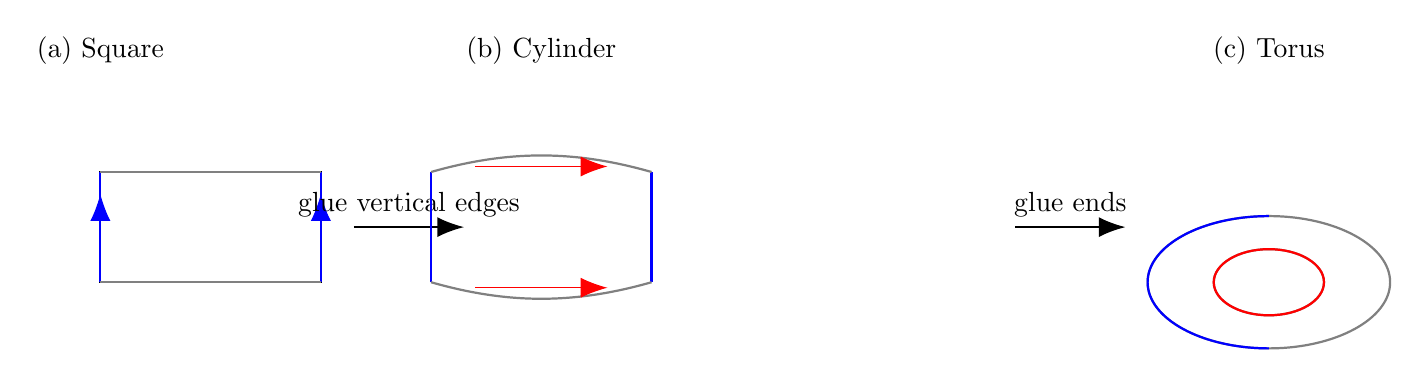
\begin{tikzpicture}[scale=1.4]
			
			% --- (a) Square ---
			\begin{scope}
				\node at (0,2.1) {(a) Square};
				
				\draw[thick] (0,0) rectangle (2,1);
				
				% vertical gluing (blue)
				\draw[thick,blue] (0,0) -- (0,1);
				\draw[thick,blue] (2,0) -- (2,1);
				\draw[blue,->] (0,0.2) -- (0,0.8);
				\draw[blue,->] (2,0.2) -- (2,0.8);
				
				% horizontal edges (no gluing yet, gray)
				\draw[thick,gray] (0,0) -- (2,0);
				\draw[thick,gray] (0,1) -- (2,1);
			\end{scope}
			
			% Arrow to cylinder
			\draw[->,thick] (2.3,0.5) -- (3.3,0.5)
			node[midway,above] {glue vertical edges};
			
			% --- (b) Cylinder ---
			\begin{scope}[xshift=4cm]
				\node at (0,2.1) {(b) Cylinder};
				
				% cylinder (side view)
				\draw[thick,blue] (-1,0) -- (-1,1);
				\draw[thick,blue] ( 1,0) -- ( 1,1);
				\draw[thick,gray] (-1,0) .. controls (-0.3,-0.2) and (0.3,-0.2) .. (1,0);
				\draw[thick,gray] (-1,1) .. controls (-0.3, 1.2) and (0.3, 1.2) .. (1,1);
				
				% arrows along top/bottom (red) for later gluing
				\draw[red,->] (-0.6,1.05) -- (0.6,1.05);
				\draw[red,->] (-0.6,-0.05) -- (0.6,-0.05);
			\end{scope}
			
			% Arrow to torus
			\draw[->,thick] (8.3,0.5) -- (9.3,0.5)
			node[midway,above] {glue ends};
			
			% --- (c) Torus ---
			\begin{scope}[xshift=10.6cm]
				\node at (0,2.1) {(c) Torus};
				
				% torus as "doughnut"
				\draw[thick,gray] (0,0)
				circle [x radius=1.1,y radius=0.6];
				\draw[thick,gray] (0,0)
				circle [x radius=0.5,y radius=0.3];
				
				% highlight one meridian (blue) and one longitude (red)
				\draw[blue,thick] (0,0.6)
				arc[start angle=90,end angle=270,
				x radius=1.1,y radius=0.6];
				\draw[red,thick] (0.5,0)
				arc[start angle=0,end angle=360,
				x radius=0.5,y radius=0.3];
			\end{scope}
			
		\end{tikzpicture}
		\caption{Building the torus: (a) start from the square $[0,1]^{2}$;
			(b) glue vertical edges to obtain a cylinder; (c) glue the two circular ends
			of the cylinder to obtain the torus.  Blue curves indicate the first gluing,
			red curves the second.}
		\label{fig:square-cylinder-torus}
	\end{figure}
	
	
	\subsection*{Explanation of Figure \ref{fig:torus-diagonal}}
	
	Figure~\ref{fig:torus-diagonal} shows two different structures on the same
	square, corresponding to two successive quotient constructions.
	
	\paragraph{1. Edge identifications: the torus.}
	Let $Q=[0,1]\times[0,1]$.  The blue and red arrows on the boundary indicate the
	usual identifications
	\[
	(0,y)\sim(1,y), \qquad (x,0)\sim(x,1), \qquad x,y\in[0,1],
	\]
	with the arrows chosen so that the gluing is orientation–preserving.  Gluing
	the vertical edges (blue) first produces a cylinder; gluing the horizontal
	edges (red) of the cylinder then produces the torus
	\[
	T^{2} \;\cong\; Q/\!\sim_{\text{edges}}.
	\]
	
	\paragraph{2. The diagonal as fixed locus of the involution.}
	Inside the square the green diagonal $\Delta$ represents the set of pairs
	$(p,q)\in S^{1}\times S^{1}$ with $p=q$.  In coordinates this is the diagonal
	\[
	\Delta=\{(p,p):p\in S^{1}\}\subset T^{2}.
	\]
	It is precisely the fixed–point set of the involution
	\[
	\tau:T^{2}\to T^{2}, \qquad \tau(p,q)=(q,p),
	\]
	which swaps the two coordinates.  Points on $\Delta$ satisfy $(p,q)=(q,p)$.
	
	\paragraph{3. Reflection across $\Delta$ as the involution $\tau$.}
	Away from $\Delta$, the involution $\tau$ identifies a point $(p,q)$ with its
	mirror image $(q,p)$ across the diagonal.  In the square model this is drawn
	as \emph{reflection across $\Delta$}: each point in one triangular half of the
	square is paired with a unique point in the other half.  The blue text
	“reflection across $\Delta$” denotes this identification.
	
	\paragraph{4. Quotient by the reflection: $\mathbb{RP}^{2}$.}
	The quotient of $T^{2}$ by the involution $\tau$ is obtained geometrically by
	identifying mirror points across the diagonal.  Topologically, the square
	modulo this reflection is a $2$–cell whose boundary comes from the diagonal,
	and after the original edge identifications this cell becomes the projective
	plane:
	\[
	T^{2}/\tau \;\cong\; \mathbb{RP}^{2}.
	\]
	
	\paragraph{5. Relation to $X \cong \mathbb{RP}^{2}\setminus\overline{D}$.}
	The diagonal $\Delta$ corresponds to unordered pairs $\{p,p\}$ on the circle.
	Removing a small open neighbourhood of $\Delta$ in $T^{2}$ corresponds, under
	the quotient by $\tau$, to removing a closed disc $\overline{D}$ from
	$\mathbb{RP}^{2}$.  Thus the space $X$ of unordered pairs $\{p,q\}$ with
	$p\neq q$ is homeomorphic to the complement of a closed disc in the projective
	plane:
	\[
	X \;\cong\; (S^{1}\times S^{1})/\tau \setminus \overline{D}
	\;\cong\; \mathbb{RP}^{2}\setminus \overline{D}.
	\]
	This is the identification used in Problem~E3.
	
	
	\section*{Problem 1: Small Metric Spaces and Isometric Embeddings}
	
	Let $(X,d)$ be a metric space.
	
	\subsection*{Statement}
	
	\begin{enumerate}[label=\textnormal{(\alph*)}]
		\item If $X=\{p_1,p_2,p_3\}$ has only three points, show that $X$ admits an
		isometric embedding into the Euclidean plane $(\mathbb{R}^2,d_{\mathrm{eucl}})$.
		
		\item Show that the four-point space
		\[
		X=\{p_1,p_2,p_3,q\}
		\]
		with distances
		\[
		d(p_i,p_j)=2L \quad(1\le i<j\le 3),\qquad
		d(p_1,q)=2L,\qquad d(p_2,q)=d(p_3,q)=L
		\]
		is a metric space which admits no isometric embedding into any Euclidean
		space $\mathbb{R}^n$.
		
		\item Let $L=\pi/4$ in \textnormal{(b)}.  Show that $X$ isometrically embeds
		in the unit sphere $(S^2,d_{S^2})\subset\mathbb{R}^3$, where $d_{S^2}$ is
		great-circle distance, and deduce that no subset of $S^2$ containing an open
		hemisphere admits an isometric embedding into the plane
		$(\mathbb{R}^2,d_{\mathrm{eucl}})$.
	\end{enumerate}
	
	\subsection*{Theory}
	
	A map $F:(X,d_X)\to(Y,d_Y)$ is an \emph{isometric embedding} if it is
	injective and
	\[
	d_Y(F(x),F(x'))=d_X(x,x')\quad\forall\,x,x'\in X.
	\]
	Any three-point metric space satisfying the triangle inequalities can be
	realised as a Euclidean triangle.  In Euclidean space, distance constraints
	give quadratic equations; for small configurations one can solve them
	explicitly and detect contradictions (e.g.\ a negative ``squared length'').
	
	On the unit sphere $S^2\subset\mathbb{R}^3$ with the intrinsic metric,
	the distance between unit vectors $u,v$ is
	\[
	d_{S^2}(u,v)=\arccos(u\cdot v),
	\]
	where $\cdot$ denotes the Euclidean dot product.  Rotations of $\mathbb{R}^3$
	preserve both $S^2$ and $d_{S^2}$, so any finite configuration can be rotated
	into a given open hemisphere.
	
	\subsection*{Solutions}
	
	\subsubsection*{(a) Three points embed into the plane}
	
	Let
	\[
	a=d(p_1,p_2),\quad b=d(p_1,p_3),\quad c=d(p_2,p_3).
	\]
	By the triangle inequality the three numbers $a,b,c$ satisfy
	\[
	a\le b+c,\quad b\le a+c,\quad c\le a+b.
	\]
	
	Place
	\[
	F(p_1)=(0,0),\qquad F(p_2)=(a,0)\in\mathbb{R}^2
	\]
	and seek $F(p_3)=(x,y)$ with
	\[
	\|F(p_3)-F(p_1)\|=b,\qquad \|F(p_3)-F(p_2)\|=c.
	\]
	Equivalently,
	\[
	x^2+y^2=b^2,\qquad (x-a)^2+y^2=c^2.
	\]
	Subtracting gives
	\[
	a^2-2ax=c^2-b^2,\qquad
	x=\frac{a^2+b^2-c^2}{2a}.
	\]
	Then
	\[
	y^2=b^2-x^2
	=\frac{(a+b+c)(a+b-c)(a-b+c)(-a+b+c)}{16a^2}\ge 0,
	\]
	by the triangle inequalities.  Hence there exists $y\in\mathbb{R}$ and an
	isometric embedding $F:X\to\mathbb{R}^2$.
	
	\subsubsection*{(b) Non-embeddability of the four-point space}
	
	Suppose, for a contradiction, that there exists an isometric embedding
	$F:X\to\mathbb{R}^n$.  Let
	\[
	P_i=F(p_i),\qquad Q=F(q).
	\]
	The points $P_1,P_2,P_3$ form an equilateral triangle of side $2L$.  After a
	rigid motion we may assume
	\[
	P_1=(0,0,0,\dots),\quad
	P_2=(2L,0,0,\dots),\quad
	P_3=(L,\sqrt{3}\,L,0,\dots).
	\]
	Write $Q=(x,y,u)$ with $(x,y)\in\mathbb{R}^2$ and $u\in\mathbb{R}^{n-2}$; set
	$\|u\|^2=U\ge0$.
	
	The distance conditions become
	\begin{align*}
		(x-2L)^2+y^2+U &= L^2, \tag{1}\\
		(x-L)^2+(y-\sqrt{3}L)^2+U &= L^2, \tag{2}\\
		x^2+y^2+U &= 4L^2. \tag{3}
	\end{align*}
	Subtracting \textnormal{(2)} from \textnormal{(1)} yields
	\[
	-2Lx+2\sqrt{3}Ly=0,\qquad x=\sqrt{3}\,y.
	\]
	Subtracting \textnormal{(1)} from \textnormal{(3)} gives
	\[
	x^2-(x-2L)^2=3L^2,\qquad 4Lx-4L^2=3L^2,
	\]
	so $x=7L/4$ and hence $y=7L/(4\sqrt{3})$.
	
	From \textnormal{(1)},
	\[
	(x-2L)^2+y^2+U=L^2
	\]
	implies
	\[
	U = L^2 - \frac{L^2}{16}-\frac{49L^2}{48}
	= -\frac{L^2}{12}<0,
	\]
	contradicting $U=\|u\|^2\ge0$.  Thus no isometric embedding of $X$ into any
	$\mathbb{R}^n$ exists.
	
	\subsubsection*{(c) Embedding into $S^2$ and hemispheres}
	
	Set $L=\pi/4$ and consider the unit sphere $S^2\subset\mathbb{R}^3$ with
	intrinsic distance
	\[
	d_{S^2}(u,v)=\arccos(u\cdot v).
	\]
	
	Choose
	\[
	P_1=(1,0,0),\quad P_2=(0,1,0),\quad P_3=(0,0,1)\in S^2.
	\]
	These are pairwise orthogonal, so
	\[
	d_{S^2}(P_i,P_j)=\arccos(0)=\frac{\pi}{2}=2L
	\quad (1\le i<j\le 3).
	\]
	Let
	\[
	Q=\left(0,\frac{1}{\sqrt{2}},\frac{1}{\sqrt{2}}\right)\in S^2.
	\]
	Then
	\[
	P_1\cdot Q=0,\qquad
	P_2\cdot Q=P_3\cdot Q=\frac{1}{\sqrt{2}},
	\]
	so
	\[
	d_{S^2}(P_1,Q)=\frac{\pi}{2}=2L,\qquad
	d_{S^2}(P_2,Q)=d_{S^2}(P_3,Q)=\frac{\pi}{4}=L.
	\]
	Therefore the map $F$ defined by $F(p_i)=P_i$, $F(q)=Q$ is an isometric
	embedding of $X$ into $(S^2,d_{S^2})$.
	
	Now let $Y\subset S^2$ contain an open hemisphere $H$.  Since rotations of
	$S^2$ are isometries and $H$ is open, we can rotate the above four-point
	configuration so that all four points lie in $H\subset Y$.  Thus $Y$
	contains a subset isometric to $X$.
	
	If there were an isometric embedding $\Phi:Y\to\mathbb{R}^2$, its restriction
	to this four-point subset would be an isometric embedding of $X$ into
	$\mathbb{R}^2$, contradicting part \textnormal{(b)}.  Hence no subset of $S^2$
	containing an open hemisphere admits an isometric embedding into the plane.
	\qedhere
	
	\paragraph{Two-point metric spaces.}
	Let $X=\{a,b\}$ with $d(a,b)=\ell>0$.  An isometric embedding into
	$\mathbb{R}$ is given by
	\[
	F(a)=0,\qquad F(b)=\ell,
	\]
	since $|F(a)-F(b)|=\ell=d(a,b)$.  Likewise, into $\mathbb{R}^2$ we may choose
	$G(a)=(0,0)$ and $G(b)=(\ell,0)$.  Any map which sends $a,b$ to points at a
	different distance, or fails to be injective (for instance $K(a)=K(b)=0$), is
	\emph{not} an isometric embedding.
	
	\paragraph{Three-point metric spaces and Euclidean triangles.}
	Let $X=\{p_1,p_2,p_3\}$ and set
	\[
	a=d(p_1,p_2),\quad b=d(p_1,p_3),\quad c=d(p_2,p_3).
	\]
	Because $d$ is a metric, the triangle inequalities hold:
	\[
	a\le b+c,\quad b\le a+c,\quad c\le a+b.
	\]
	We now construct an isometric embedding $F:X\to\mathbb{R}^2$.
	
	Place
	\[
	F(p_1)=(0,0),\qquad F(p_2)=(a,0),
	\]
	and write $F(p_3)=(x,y)$.  The distance constraints become
	\[
	x^2+y^2=b^2,\qquad (x-a)^2+y^2=c^2.
	\]
	Subtracting the equations gives
	\[
	a^2-2ax=c^2-b^2,\qquad
	x=\frac{a^2+b^2-c^2}{2a}.
	\]
	Then
	\[
	y^2=b^2-x^2
	=b^2-\left(\frac{a^2+b^2-c^2}{2a}\right)^2
	=\frac{(a+b+c)(a+b-c)(a-b+c)(-a+b+c)}{16a^2}\ge 0.
	\]
	Thus $y\in\mathbb{R}$ exists and the three points
	\[
	F(p_1)=(0,0),\quad F(p_2)=(a,0),\quad F(p_3)=(x,y)
	\]
	form a Euclidean triangle whose side lengths are exactly
	$a,b,c$.  Hence every three-point metric space satisfying the triangle
	inequalities can be realised as a Euclidean triangle via an isometric
	embedding into $\mathbb{R}^2$.
	
	\subsection*{Embeddings, isometric embeddings, and injectivity}
	
	Let $(X,d_X)$ and $(Y,d_Y)$ be metric spaces.
	
	\paragraph{Topological embeddings.}
	A \emph{topological embedding} is a continuous map $f:X\to Y$ which is
	injective and a homeomorphism from $X$ onto its image $f(X)$, equipped with
	the subspace topology.  Such a map may distort distances; it preserves only
	the topology.
	
	\paragraph{Isometric embeddings.}
	An \emph{isometric embedding} is a map $f:X\to Y$ satisfying
	\[
	d_Y(f(x),f(y)) = d_X(x,y)\qquad\text{for all }x,y\in X.
	\]
	This condition preserves the metric exactly.  In particular, if $f$ is
	distance-preserving then it is automatically injective: if $f(x)=f(y)$ then
	\[
	0 = d_Y(f(x),f(y)) = d_X(x,y),
	\]
	and since $d_X$ is a metric we must have $x=y$.  Thus an isometric embedding
	is a special kind of topological embedding which preserves all distances and
	hence all geometric information encoded by the metric.
	
	\paragraph{Why injectivity?}
	When we speak of an ``embedding'' we want to regard $X$ as a copy of a
	subspace of $Y$.  This requires a one-to-one correspondence between points of
	$X$ and points of the image $f(X)\subset Y$; otherwise different points of $X$
	would be identified in $Y$ and the structure of $X$ would be lost.  For
	general topological embeddings injectivity is imposed by definition; for
	isometric embeddings it follows automatically from the metric property.
	
	
	
	\section*{Problem 2: Allowable parametrisations and first fundamental form}
	
	Show that each of the following parametrisations $\sigma : U \to \mathbb{R}^3$
	is allowable, find the first fundamental form and sketch the image of $\sigma$.
	\begin{enumerate}[label=\textnormal{(\alph*)}]
		\item $U = \{(u,v)\in\mathbb{R}^2 \mid u>v\}$,
		\quad $\sigma(u,v) = (u+v,\,2uv,\,u^2+v^2)$;
		\item $U = \{(r,z)\in\mathbb{R}^2 \mid r>0\}$,
		\quad $\sigma(r,z) = (r\cos z,\,r\sin z,\,z)$.
	\end{enumerate}
	
	
	
	% Needs in preamble:
	% \usepackage{tikz}
	% \usetikzlibrary{arrows.meta}
	
	\begin{figure}[h]
		\centering
		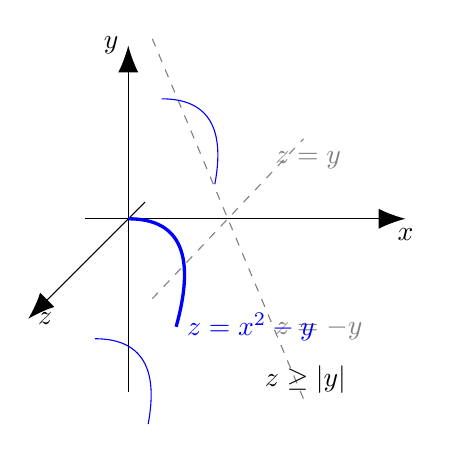
\begin{tikzpicture}[scale=1.1]
			% axes
			\draw[->] (-0.5,0,0) -- (3.2,0,0) node[below] {$x$};
			\draw[->] (0,-2,0) -- (0,2,0) node[left] {$y$};
			\draw[->] (0,0,-0.5) -- (0,0,3) node[right] {$z$};
			
			% planes z=y and z=-y (projected)
			\draw[dashed,gray] (-0.3,-1.5,-1.5) -- (2.6,1.5,1.5) node[near end,above right] {$z=y$};
			\draw[dashed,gray] (-0.3,1.5,-1.5) -- (2.6,-1.5,1.5) node[near end,below right] {$z=-y$};
			
			% parabolic cylinder z = x^2 - y : draw a few 'generating' parabolas
			\foreach \yy in {-1,0,1}{
				\draw[blue,smooth,domain=0:1.6,variable=\xx]
				plot ({\xx},{\yy},{\xx*\xx - \yy});
			}
			
			% one highlighted curve at y=0
			\draw[blue,very thick,smooth,domain=0:1.8,variable=\xx]
			plot ({\xx},{0},{\xx*\xx}) node[right] {$z=x^2-y$};
			
			% text
			\node at (2.7,-1.2,1.7) {$z\ge |y|$};
		\end{tikzpicture}
		\caption{Schematic sketch of the image of $\sigma(u,v)=(u+v,2uv,u^2+v^2)$:
			a parabolic sheet $z=x^2-y$ cut by $z\ge |y|$.}
		\label{fig:sigma-parabolic}
	\end{figure}
	
	
	\begin{figure}[h]
		\centering
		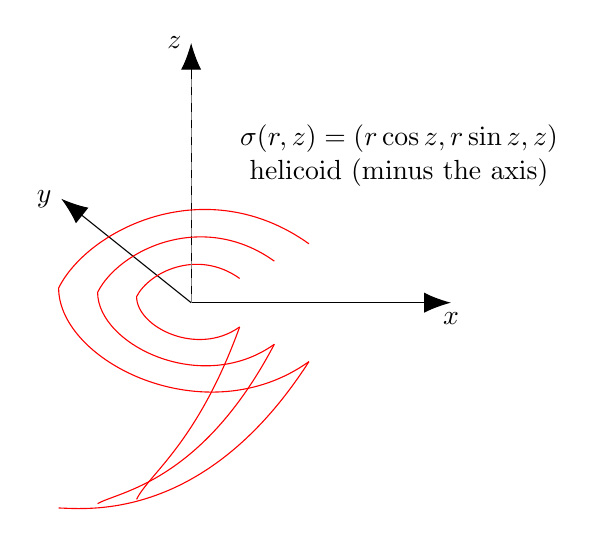
\begin{tikzpicture}[scale=1.1]
			% 3D-ish axes in oblique projection
			\draw[->] (0,0) -- (3,0) node[below] {$x$};
			\draw[->] (0,0) -- (-1.5,1.2) node[left] {$y$};
			\draw[->] (0,0) -- (0,3) node[left] {$z$};
			
			% a few helices with different radii (very schematic)
			\foreach \r in {0.7,1.2,1.7}{
				\draw[red,smooth]
				( { \r*0.8 }, { \r*0.4 })  % starting point near z=0
				.. controls ({\r*0.1},{\r*0.9}) and ({-\r*0.7},{\r*0.5})
				.. ({-\r*0.9},{\r*0.1})
				.. controls ({-\r*0.9},{-\r*0.4}) and ({\r*0.1},{-\r*0.9})
				.. ({\r*0.8},{-\r*0.4});
				\draw[red,smooth]
				({\r*0.8},{-\r*0.4}) .. controls
				({\r*0.1},{-0.9*\r-1.0}) and ({-\r*0.7},{-0.4*\r-1.7})
				.. ({-\r*0.9},{-0.1*\r-2.2});
			}
			
			% hint of the axis
			\draw[dashed,gray] (0,0) -- (0,2.6);
			
			\node at (2.4,1.9) {$\sigma(r,z)=(r\cos z,r\sin z,z)$};
			\node at (2.4,1.5) {helicoid (minus the axis)};
		\end{tikzpicture}
		\caption{Schematic sketch of the image of $\sigma(r,z)=(r\cos z,r\sin z,z)$:
			a helicoid obtained by helices of radius $r$ as $r>0$ varies.}
		\label{fig:sigma-helicoid}
	\end{figure}
	
	\subsection*{(a) The parametrisation $\sigma(u,v)=(u+v,2uv,u^2+v^2)$}
	
	\paragraph{Regularity.}
	We have
	\[
	\sigma_u = (1,2v,2u),\qquad
	\sigma_v = (1,2u,2v).
	\]
	Their cross product is
	\[
	\sigma_u\times\sigma_v
	= \bigl(4(v^2-u^2),\,2(u-v),\,2(u-v)\bigr),
	\]
	which vanishes only when $u=v$.  Since $U=\{u>v\}$ excludes $u=v$, the vectors
	$\sigma_u,\sigma_v$ are linearly independent at every point of $U$, and
	$\sigma$ is a regular parametrisation.
	
	\paragraph{Injectivity.}
	If $\sigma(u,v)=\sigma(u',v')$, write
	\[
	(u+v,2uv,u^2+v^2) = (x,y,z).
	\]
	Then
	\[
	u+v=x,\qquad uv=\frac{y}{2},\qquad u^2+v^2=z.
	\]
	The numbers $u,v$ are the (unordered) roots of $t^2-xt+\frac{y}{2}=0$, so the
	set $\{u,v\}$ is determined by $(x,y,z)$.  The condition $u>v$ fixes the
	ordering of the roots, so $(u,v)$ is uniquely determined and $\sigma$ is
	injective on $U$.  Hence $\sigma$ is an allowable parametrisation.
	
	\paragraph{First fundamental form.}
	We compute
	\[
	E = \langle\sigma_u,\sigma_u\rangle
	= 1+4(u^2+v^2),
	\]
	\[
	F = \langle\sigma_u,\sigma_v\rangle
	= 1+8uv,
	\]
	\[
	G = \langle\sigma_v,\sigma_v\rangle
	= 1+4(u^2+v^2).
	\]
	Thus the first fundamental form is
	\[
	I = E\,du^2 + 2F\,du\,dv + G\,dv^2
	= \bigl(1+4(u^2+v^2)\bigr)(du^2+dv^2) + 2(1+8uv)\,du\,dv.
	\]
	
	\paragraph{Image.}
	Let $(x,y,z)=\sigma(u,v)=(u+v,2uv,u^2+v^2)$.  Then
	\[
	x^2 = (u+v)^2 = u^2+2uv+v^2 = (u^2+v^2)+2uv = z+y,
	\]
	so the image lies on the parabolic surface
	\[
	z = x^2 - y.
	\]
	Moreover
	\[
	z = u^2+v^2 \ge 2|uv| = |y|.
	\]
	Hence the image of $\sigma$ is the subset
	\[
	S = \{(x,y,z)\in\mathbb{R}^3 : z = x^2 - y,\; z\ge |y|\},
	\]
	a parabolic sheet cut by the two planes $z=\pm y$ (corresponding to the
	condition $u>v$).
	
	\subsection*{(b) The parametrisation $\sigma(r,z)=(r\cos z,r\sin z,z)$}
	
	\paragraph{Regularity and injectivity.}
	We have
	\[
	\sigma_r = (\cos z,\sin z,0),\qquad
	\sigma_z = (-r\sin z,r\cos z,1).
	\]
	Their cross product is
	\[
	\sigma_r\times\sigma_z
	= (\sin z,-\cos z,r),
	\]
	which is never zero for $r>0$.  Thus $\sigma$ is regular on $U$.
	
	If $\sigma(r,z)=\sigma(r',z')$, the third coordinate gives $z=z'$; for this
	fixed $z$ we then have $(r\cos z,r\sin z)=(r'\cos z,r'\sin z)$ and hence
	$r=r'$.  Therefore $\sigma$ is injective on $U$ and hence allowable.
	
	\paragraph{First fundamental form.}
	We compute
	\[
	E = \langle\sigma_r,\sigma_r\rangle
	= \cos^2 z + \sin^2 z = 1,
	\]
	\[
	F = \langle\sigma_r,\sigma_z\rangle
	= \cos z(-r\sin z) + \sin z(r\cos z) = 0,
	\]
	\[
	G = \langle\sigma_z,\sigma_z\rangle
	= r^2\sin^2 z + r^2\cos^2 z + 1 = r^2+1.
	\]
	Thus
	\[
	I = dr^2 + (r^2+1)\,dz^2.
	\]
	
	\paragraph{Image.}
	From the first two coordinates we obtain $x^2+y^2=r^2$ and from the third
	coordinate $z=z$.  For each fixed $r>0$, the curve $z\mapsto(r\cos z,r\sin z,z)$
	is a helix on the cylinder $x^2+y^2=r^2$.  As $r$ varies these helices sweep
	out the classical helicoid (minus the axis $r=0$).
	
	
	\subsection*{First Fundamental Form}
	
	Let $\sigma : U \subset \mathbb{R}^2 \to \mathbb{R}^3$ be a smooth regular
	parametrisation of a surface.  The tangent vectors at $(u,v)\in U$ are
	\[
	\sigma_u = \frac{\partial \sigma}{\partial u},
	\qquad
	\sigma_v = \frac{\partial \sigma}{\partial v}.
	\]
	The \emph{first fundamental form} is the Riemannian metric on the surface
	induced by the Euclidean dot product of $\mathbb{R}^3$.  It is the quadratic
	form
	\[
	I = E\,du^2 + 2F\,du\,dv + G\,dv^2,
	\]
	where
	\[
	E = \langle \sigma_u,\sigma_u\rangle, \qquad
	F = \langle \sigma_u,\sigma_v\rangle, \qquad
	G = \langle \sigma_v,\sigma_v\rangle.
	\]
	For a curve $\gamma(t)=\sigma(u(t),v(t))$ on the surface, its speed is
	\[
	\|\gamma'(t)\|^2
	= E u'(t)^2 + 2F u'(t)v'(t) + G v'(t)^2.
	\]
	Thus the first fundamental form contains all metric information of the
	surface (lengths, angles, areas).
	
	\subsection*{Second Fundamental Form}
	
	Let $\sigma : U \subset \mathbb{R}^2 \to \mathbb{R}^3$ be a smooth regular
	parametrisation of a surface.  The unit normal vector field is
	\[
	N = \frac{\sigma_u \times \sigma_v}{\|\sigma_u \times \sigma_v\|}.
	\]
	The \emph{second fundamental form} of the surface is the quadratic form
	on tangent vectors defined by
	\[
	\mathrm{II}(u,v)
	= \langle\sigma_{uu},N\rangle\,du^2
	+ 2\langle\sigma_{uv},N\rangle\,du\,dv
	+ \langle\sigma_{vv},N\rangle\,dv^2.
	\]
	We set
	\[
	e = \langle\sigma_{uu},N\rangle,\qquad
	f = \langle\sigma_{uv},N\rangle,\qquad
	g = \langle\sigma_{vv},N\rangle.
	\]
	Thus
	\[
	\mathrm{II} = e\,du^2 + 2f\,du\,dv + g\,dv^2.
	\]
	
	The second fundamental form measures the extrinsic curvature of the surface.
	For a curve $\gamma(t)=\sigma(u(t),v(t))$ on the surface, its normal
	curvature is
	\[
	k_n = \frac{\mathrm{II}}{\mathrm{I}}.
	\]
	The principal curvatures are the eigenvalues of the shape operator, and the
	Gaussian and mean curvatures are given by
	\[
	K = \frac{eg - f^2}{EG - F^2},
	\qquad
	H = \frac{1}{2}\,\frac{E g - 2F f + G e}{E G - F^2},
	\]
	where $I = E\,du^2 + 2F\,du\,dv + G\,dv^2$ is the first fundamental form.
	
	

\subsection*{Problem 3: Mercator's projection of the sphere}

\textbf{Problem statement.}
Mercator's projection of the unit sphere $S^{2}\subset\mathbb{R}^{3}$ is the
chart whose inverse is the local parametrization
\[
\sigma(u,v) = (\operatorname{sech}u\cos v,\ \operatorname{sech}u\sin v,\ \tanh u).
\]
\begin{enumerate}
	\item Show that this parametrization determines an allowable chart on
	the complement of a longitude of the sphere.
	\item Prove that, under this chart, lines of longitude and latitude are
	mapped to straight lines in the plane.
	\item Show that the resulting map preserves angles but does not preserve areas.
\end{enumerate}

\medskip
\textbf{Remark.}

The local parametrization
\[
\sigma(u,v) = (\operatorname{sech}u\cos v,\ \operatorname{sech}u\sin v,\ \tanh u)
\]
maps the parameter plane into $S^2$. The actual Mercator map used in
cartography is the inverse chart
\[
\varphi = \sigma^{-1}: S^2\setminus\{\text{one longitude}\}\to\mathbb{R}^2,
\]
given by
\[
\varphi(x,y,z) = \bigl(u,v\bigr)
= \bigl(\operatorname{artanh}(z),\,\operatorname{atan2}(y,x)\bigr).
\]
In geographic coordinates $(\phi,\lambda)$ (latitude, longitude) one has
$z=\sin\phi$, so $u=\operatorname{artanh}(\sin\phi)$ and
\[
x = R\lambda,\qquad y = R\,\operatorname{artanh}(\sin\phi)
= R\ln\Bigl(\tan\bigl(\tfrac{\pi}{4}+\tfrac{\phi}{2}\bigr)\Bigr),
\]
which are the usual Mercator projection formulas.


\medskip
\textbf{Theory.}
A smooth map $\sigma:V\subset\mathbb{R}^{2}\to S^{2}$ is a (local)
parametrization of $S^{2}$ if it is regular, i.e.
$\sigma_u\times\sigma_v\neq 0$ everywhere.
The induced metric (first fundamental form) is
\[
I = E\,du^{2} + 2F\,du\,dv + G\,dv^{2},
\quad
E = \sigma_u\cdot\sigma_u,\quad
F = \sigma_u\cdot\sigma_v,\quad
G = \sigma_v\cdot\sigma_v.
\]
If $I$ has the form
\[
I = \lambda(u,v)^{2}\big(du^{2}+dv^{2}\big),\qquad \lambda>0,
\]
then the parametrization is \emph{conformal}: the corresponding chart
preserves angles. The area element on the surface in the coordinates
$(u,v)$ is
\[
dA = \sqrt{EG-F^{2}}\,du\,dv = |\sigma_u\times\sigma_v|\,du\,dv.
\]

\medskip
\textbf{Solution.}

\emph{(1) Image, domain and regularity.}
First, for all $(u,v)$ we have
\[
\begin{aligned}
	x^{2}+y^{2}+z^{2}
	&= \operatorname{sech}^{2}u\cos^{2}v
	+ \operatorname{sech}^{2}u\sin^{2}v + \tanh^{2}u \\
	&= \operatorname{sech}^{2}u(\cos^{2}v+\sin^{2}v) + \tanh^{2}u \\
	&= \operatorname{sech}^{2}u + \tanh^{2}u = 1,
\end{aligned}
\]
so $\sigma$ takes values in $S^{2}$.

Take
\[
V = \{(u,v)\in\mathbb{R}^{2} : -\pi < v < \pi\}.
\]
For any point $(x,y,z)\in S^{2}$ with $(x,y)\neq(-\sqrt{1-z^{2}},0)$ there is a
unique $v\in(-\pi,\pi)$ such that
\[
\cos v = \frac{x}{\sqrt{x^{2}+y^{2}}},\qquad
\sin v = \frac{y}{\sqrt{x^{2}+y^{2}}},
\]
and setting
\[
u = \operatorname{artanh}(z)
\]
gives
\[
x = \operatorname{sech}u\cos v,\quad
y = \operatorname{sech}u\sin v,\quad
z = \tanh u.
\]
Thus $\sigma$ is a bijection from $V$ onto $S^{2}\setminus L$, where
\[
L = \{(-\sqrt{1-z^{2}},0,z) : -1<z<1\}
\]
is the longitude corresponding to $v=\pm\pi$.
Its inverse $\sigma^{-1}$ is therefore a chart on $S^{2}\setminus L$.

To see that $\sigma$ is regular, compute
\[
\begin{aligned}
	\sigma_u &= (-\operatorname{sech}u\tanh u\cos v,\
	-\operatorname{sech}u\tanh u\sin v,\
	\operatorname{sech}^{2}u),\\[1mm]
	\sigma_v &= (-\operatorname{sech}u\sin v,\
	\operatorname{sech}u\cos v,\ 0),
\end{aligned}
\]
and hence
\[
\begin{aligned}
	E &= \sigma_u\cdot\sigma_u
	= \operatorname{sech}^{2}u\tanh^{2}u + \operatorname{sech}^{4}u
	= \operatorname{sech}^{2}u,\\
	G &= \sigma_v\cdot\sigma_v
	= \operatorname{sech}^{2}u(\sin^{2}v+\cos^{2}v)
	= \operatorname{sech}^{2}u,\\
	F &= \sigma_u\cdot\sigma_v = 0.
\end{aligned}
\]
Thus
\[
EG - F^{2} = \operatorname{sech}^{4}u > 0,
\]
so $\sigma$ is regular and gives an allowable parametrization of
$S^{2}\setminus L$.

\medskip
\emph{(2) Longitudes and latitudes.}
A line of longitude on $S^{2}$ is obtained by fixing $v=v_{0}$ and letting $u$
vary:
\[
\gamma(t) = \sigma(u(t),v_{0}).
\]
In the parameter domain $V$ this is the straight vertical line
$\{v=v_{0}\}$. A line of latitude (parallel) is obtained by fixing
$u=u_{0}$ and letting $v$ vary; it corresponds in $V$ to the horizontal line
$\{u=u_{0}\}$. Therefore the chart $\sigma^{-1}$ sends both longitudes and
latitudes to straight lines in the plane.

\medskip
\emph{(3) Angle preservation and area distortion.}
From the above computation,
\[
I = E\,du^{2} + 2F\,du\,dv + G\,dv^{2}
= \operatorname{sech}^{2}u\,(du^{2}+dv^{2}).
\]
The first fundamental form is thus conformal to the Euclidean metric on
$\mathbb{R}^{2}$. Consequently, the chart $\sigma^{-1}$ preserves angles
between curves on $S^{2}$: the angle between two curves on the sphere equals
the Euclidean angle between their images in the $(u,v)$-plane.

The area element on the sphere in Mercator coordinates is
\[
dA_{S} = \sqrt{EG-F^{2}}\,du\,dv
= \operatorname{sech}^{2}u\,du\,dv.
\]
But the Euclidean area element in the map plane is $du\,dv$, so the ratio
between map area and spherical area is
\[
\frac{dA_{\text{map}}}{dA_{S}} = \frac{1}{\operatorname{sech}^{2}u}
= \cosh^{2}u,
\]
which depends on $u$. Hence Mercator's projection is not area preserving:
regions at high latitudes (large $|u|$) appear greatly enlarged compared to
regions near the equator.

\medskip
\textbf{Examples and remarks.}
\begin{itemize}
	\item The equator has $z=0$, hence $u=0$, so it maps to the horizontal line
	$u=0$ in the plane.
	\item A parallel at latitude $\phi$ satisfies $z=\sin\phi$, so
	$u=\operatorname{artanh}(\sin\phi)$; thus each parallel is a horizontal line
	$u=\text{const}$ on the Mercator map.
	\item At latitude $\phi=60^\circ$, one has $\cos\phi = 1/2$, so
	$\operatorname{sech}u=1/2$ and $\cosh u = 2$; areas are enlarged by a factor
	$\cosh^{2}u=4$ compared to the sphere, illustrating the strong area
	distortion of the Mercator projection near the poles.
\end{itemize}

\begin{figure}[h]
	\centering
	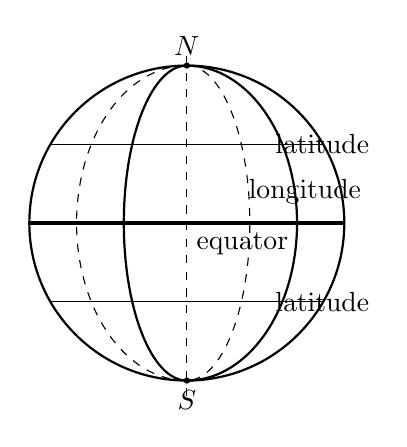
\begin{tikzpicture}[scale=2]
		% Sphere (side view -> circle)
		\draw[thick] (0,0) circle (1);
		
		% Axis (north–south)
		\draw[dashed] (0,-1.1) -- (0,1.1);
		\fill (0,1) circle (0.02) node[above] {$N$};
		\fill (0,-1) circle (0.02) node[below] {$S$};
		
		% Equator
		\draw[very thick] (-1,0) -- (1,0);
		\node[below right] at (0,0) {equator};
		
		% A few parallels (latitudes)
		\foreach \h/\labelpos in {0.5/right, -0.5/right}{
			% intersection with circle
			\pgfmathsetmacro{\x}{sqrt(1-\h*\h)}
			\draw (-\x,\h) -- (\x,\h);
		}
		\node[right] at (0.5,0.5) {latitude};
		\node[right] at (0.5,-0.5) {latitude};
		
		% A few meridians (longitudes) as ellipses
		% front meridians (solid)
		\draw[thick] (0,1) arc[start angle=90,end angle=270,
		x radius=0.4, y radius=1];
		\draw[thick] (0,1) arc[start angle=90,end angle=-90,
		x radius=0.7, y radius=1];
		
		% back meridians (dashed)
		\draw[dashed] (0,1) arc[start angle=90,end angle=270,
		x radius=0.7, y radius=1];
		\draw[dashed] (0,1) arc[start angle=90,end angle=-90,
		x radius=0.4, y radius=1];
		
		\node at (0.75,0.2) {longitude};
	\end{tikzpicture}
	\caption{Sphere with lines of longitude (meridians) and latitude (parallels).}
\end{figure}


	\begin{figure}[h]
		\centering
		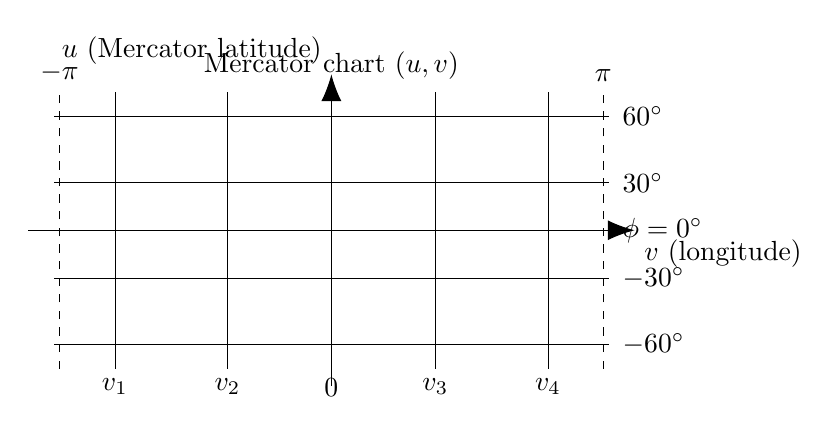
\begin{tikzpicture}[scale=1.1]
			% Axes
			\draw[->] (-3.5,0) -- (3.5,0) node[below right] {$v$ (longitude)};
			\draw[->] (0,-1.8) -- (0,1.8) node[above left] {$u$ (Mercator latitude)};
			
			% Domain boundary (approx -\pi < v < \pi)
			\draw[dashed] (-3.14,-1.6) -- (-3.14,1.6)
			node[above] {$-\pi$};
			\draw[dashed] ( 3.14,-1.6) -- ( 3.14,1.6)
			node[above] {$\pi$};
			
			% Vertical grid lines = longitudes v = const
			\foreach \x/\lab in {-2.5/{$v_1$}, -1.2/{$v_2$}, 0/{$0$}, 1.2/{$v_3$}, 2.5/{$v_4$}}{
				\draw[very thin] (\x,-1.6) -- (\x,1.6);
				\node[below] at (\x,-1.6) {\lab};
			}
			
			% Horizontal grid lines = latitudes u = const
			% approximate values: 0, ±0.55 (≈30°), ±1.32 (≈60°)
			\foreach \y/\txt in {
				0/{$\phi=0^\circ$},
				0.55/{$30^\circ$},
				-0.55/{$-30^\circ$},
				1.32/{$60^\circ$},
				-1.32/{$-60^\circ$}
			}{
				\draw[very thin] (-3.2,\y) -- (3.2,\y);
				\node[right] at (3.25,\y) {\txt};
			}
			
			% Label
			\node at (0,1.9) {Mercator chart $(u,v)$};
		\end{tikzpicture}
		\caption{Mercator projection: longitudes and latitudes become straight lines
			in the $(u,v)$-plane. The spacing of latitudes increases with $|u|$, so areas
			near the poles are greatly magnified.}
	\end{figure}
	
	\end{document}
